\documentclass[12pt, reqno, a4paper]{amsart}
%\def\pgfsysdriver{pgfsys-dvipdfmx.def}
\usepackage[dvipdfm]{graphicx}
\usepackage{amsmath, amsthm, amsfonts, amssymb, mathrsfs}
\usepackage{extarrows}
\usepackage{color, ulem}
\usepackage[all]{xy}
\usepackage{tikz-cd, tikz}
\usetikzlibrary{cd, decorations.pathmorphing, arrows.meta, positioning, calc}
\usepackage{fullpage} 
\usepackage{bm, bbm}
\usepackage{dashbox}
\usepackage{halloweenmath}
\usepackage{mathtools}
%
% Macros
%
\def\til#1{\widetilde{#1}} % tilde
\def\udl#1{\underline{#1}} % underline
\def\uudl#1{\uuline{#1}} % double underline
\def\ovl#1{\overline{#1}} % overline
\def\what#1{\widehat{#1}} % widehat
%
% arrows
%
\def\longto{\longrightarrow}
\def\longhookrightarrow{\lhook\joinrel\longto}
\def\longhookleftarrow{\longleftarrow\joinrel\rhook}
\def\biguparrow{\vphantom{\bigg|}\Big\uparrow}
\def\bigdownarrow{\vphantom{\bigg|}\Big\downarrow}
%
\def\ot{\leftarrow}
\def\eqdef{\stackrel{\textrm{def}}{=}} % "def" on the equal-sign
\def\simto{\stackrel{\sim}{\rightarrow}} % isom and categorical equiv.
\def\simot{\stackrel{\sim}{\leftarrow}} % isom and categorical equiv.
\def\simlongto{\stackrel{\sim}{\longrightarrow}} % long version of simto
\def\simlongot{\stackrel{\sim}{\longleftarrow}} % long version of simto
\def\acton{\curvearrowright} % action of groups on ###
\def\surjto{\twoheadrightarrow}
\def\surjot{\twoheadleftarrow}
\def\surjlongto{\relbar\joinrel\twoheadrightarrow}
\def\surjlongot{\twoheadleftarrow\joinrel\relbar}
\def\injto{\hookrightarrow}
\def\injlongto{\longhookrightarrow}
\def\injlongot{\longhookleftarrow}
\newcommand{\longdashrightarrow}{\begin{tikzcd}[cramped,sep=scriptsize,ampersand replacement=\&]{}\arrow[r, dashed]\&{}\end{tikzcd}}
\def\sqto{\rightsquigarrow}
\def\sqot{\leftsquigarrow}
\def\sqlongto{\longrightsquigarrow}
%
% Blackboard bold cap-alphabets
%
\def\bN{\mathbb{N}} % set of natural numbers
\def\bZ{\mathbb{Z}} % set of integers
\def\bQ{\mathbb{Q}} % set of rational numbers
\def\bR{\mathbb{R}} % set of real numbers
\def\bC{\mathbb{C}} % set of complex numbers
\def\bF{\mathbb{F}} % finite field
\def\bG{\mathbb{G}}
\def\bM{\mathbb{M}}
\def\bP{\mathbb{P}}
\def\bA{\mathbb{A}}
\def\bD{\mathbb{D}}
\def\bV{\mathbb{V}}
%
% caligraphic cap-alphabets
%
\def\cA{{\mathcal{A}}}
\def\cB{{\mathcal{B}}}
\def\cC{{\mathcal{C}}}
\def\cD{{\mathcal{D}}}
\def\cE{{\mathcal{E}}}
\def\cF{{\mathcal{F}}}
\def\cS{{\mathcal{S}}}
\def\cL{{\mathcal{L}}}
\def\cM{\mathcal{M}}
\def\cI{{\mathcal{I}}}
\def\cH{{\mathcal{H}}}
\def\cO{\mathcal{O}} % structure sheaf
\def\cP{{\mathcal{P}}}
\def\cU{\mathcal{U}}
\def\cY{\ddot{\mathcal{Y}}}
\def\cZ{{\mathcal{Z}}}
%
% fraktur cap-alphabets
%
\def\fD{{\mathfrak{D}}}
\def\fF{{\mathfrak{F}}}
\def\fT{{\mathfrak{T}}}
\def\fS{{\mathfrak{S}}}
\def\fm{\mathfrak{m}} % maximal ideal
\def\fn{\mathfrak{n}}
\def\fp{\mathfrak{p}} % prime ideal
\def\fq{\mathfrak{q}}
\def\fa{\mathfrak{a}}
\def\fb{\mathfrak{b}}
\def\fc{\mathfrak{c}}
%
% Some more styled alphabets
%
\def\hbZ{\what{\bZ}} % profinite completion of \bZ
\def\ubZ{\udl{\bZ}} % underline \bZ
\def\ubV{\udl{\bV}} % underline \bV
\def\ubF{\udl{\bF}} % underline \bF
\def\uX{\udl{X}} % underline X
\def\uY{\udl{Y}} % underline Y
\def\uC{\udl{C}} % underline C
\def\uV{\udl{\bV}} % underline V
\def\uv{\udl{v}} % underline V
\def\uuX{\uudl{X}{}} % double underline X
\def\uuY{\uudl{Y}{}} % double underline Y
\def\uuC{\uudl{C}{}} % double underline C
\def\uaX{\underscriptrightarrow{X}} % underarrow X
\def\uaY{\underscriptrightarrow{Y}} % underarrow Y
\def\uaC{\underscriptrightarrow{C}} % underarrow C
\def\ddY{\ddot{Y}}\def\dduuY{\ddot{\uuY}}
%
% Additional common shorthand
%
\def\La{\Lambda} % Capital lambda
\def\la{\lambda} % lambda
\def\dt{\delta} % delta
\def\ep{\epsilon} % epsilon
\def\uep{\udl{\ep}} %underlined epsilon
\def\vep{\varepsilon} % varepsilon
\def\uvep{\udl{\vep}} % underlined varepsilon
\def\bone{\mathbbm{1}}
\def\bmu{\bm{\mu}}
\def\xmu{\times\bmu}
\def\infH{{}_{\infty}H} % limit cohomology
\def\infuuth{{}_{\infty}\uudl{\theta}}
%
% Several super- & subscripts
%
\def\mr{\mathrm{mr}} 
\def\sp{\mathrm{sp}}
\def\cl{\mathrm{cl}} 
\def\an{\mathrm{an}}
\def\gp{\mathrm{gp}}
\def\tor{\mathrm{tor}}
\def\et{\textrm{\'et}}
\def\flgp{\mathfrak{lgp}}
\def\bad{\mathrm{bad}} 
\def\good{\mathrm{good}} 
\def\NA{0} % subscript for "non-archimedean"
\def\Ar{\infty} % subscript for "archimedean"
%
% Common math operators
%
\DeclareMathOperator{\id}{id}
\DeclareMathOperator{\Ker}{Ker}
\DeclareMathOperator{\Cok}{Cok}
\DeclareMathOperator{\Image}{Im}
\DeclareMathOperator{\codim}{codim}
\DeclareMathOperator{\Ob}{Ob}
\DeclareMathOperator{\divisor}{div}
\DeclareMathOperator{\Spec}{Spec}
\DeclareMathOperator{\Sp}{Sp}
\DeclareMathOperator{\Spm}{Spm}
\DeclareMathOperator{\Proj}{Proj}
\DeclareMathOperator{\Frac}{Frac}
\DeclareMathOperator{\Hom}{Hom}
\DeclareMathOperator{\Isom}{Isom}
\DeclareMathOperator{\Aut}{Aut}
\DeclareMathOperator{\Inn}{Inn}
\DeclareMathOperator{\Out}{Out}
\DeclareMathOperator{\Sym}{Sym}
\DeclareMathOperator{\Pic}{Pic}
\DeclareMathOperator{\Div}{Div}
\DeclareMathOperator{\GL}{GL}
\DeclareMathOperator{\SL}{SL}
\DeclareMathOperator{\Gal}{Gal}
\DeclareMathOperator{\Ism}{Ism}
\DeclareMathOperator{\red}{red}
\DeclareMathOperator{\ord}{ord}
\DeclareMathOperator{\hgt}{ht}
\DeclareMathOperator{\height}{ht}
\DeclareMathOperator{\vol}{vol}
\DeclareMathOperator{\logvol}{log-vol}
\DeclareMathOperator{\tmod}{mod}
\DeclareMathOperator{\length}{length}
\DeclareMathOperator*{\tsum}{{\textstyle \sum}}
%
% Some special math operators
%
\DeclareMathOperator{\mult}{mult}
\DeclareMathOperator{\Kummer}{Kmm}
\DeclareMathOperator{\ev}{ev}
\DeclareMathOperator{\gr}{G}
\DeclareMathOperator{\lp}{lp}
\DeclareMathOperator{\tp}{tp}
\DeclareMathOperator{\temp}{temp}
\DeclareMathOperator{\hol}{hol}
\DeclareMathOperator{\flog}{\mathfrak{log}}
\DeclareMathOperator{\logdiff}{log-diff}
\DeclareMathOperator{\logcond}{log-cond}
\DeclareMathOperator{\PF}{PF}
\DeclareMathOperator{\pilot}{pilot}
\DeclareMathOperator{\HodgeTheater}{\mathcal{HT}}
\DeclareMathOperator{\Ve}{Vert}
\DeclareMathOperator{\Cusp}{Cusp}
\DeclareMathOperator{\LabCusp}{LabCusp}
\DeclareMathOperator{\sLabCusp}{\mathsf{LabCusp}}
%\DeclareMathOperator{\BPS}{BPS}
\DeclareMathOperator{\VC}{VC}
\DeclareMathOperator{\LVC}{LVC}
\DeclareMathOperator{\LocVC}{LocVC}
\DeclareMathOperator{\LocLVC}{LocLVC}
\DeclareMathOperator{\Frob}{Frob}
\DeclareMathOperator{\FI}{FI}
\DeclareMathOperator{\hLS}{hLS}
\DeclareMathOperator{\MU}{MU}
\DeclareMathOperator{\MF}{MF}
\DeclareMathOperator{\ME}{ME}
\DeclareMathOperator{\GM}{GM}
\DeclareMathOperator{\GNM}{GNM}
\DeclareMathOperator{\VG}{VG}
\DeclareMathOperator{\Ind}{Ind}
\DeclareMathOperator{\plpl}{\text{++}}
%
% Special symbols with upper-left superscript
%
\NewDocumentCommand{\LS}{o}{\IfNoValueTF{#1}{\cI}{\prescript{#1}{}{}{\cI}}}
%
\NewDocumentCommand{\OO}{o}{\IfNoValueTF{#1}{\cO{}}{\prescript{#1}{}{}{\cO}{}}}
\NewDocumentCommand{\OOx}{o}{\IfNoValueTF{#1}{\cO{}^{\times}}{\prescript{#1}{}{}{\cO}{}^{\times}}}
\NewDocumentCommand{\OOmu}{o}{\IfNoValueTF{#1}{\cO{}^{\bm{\mu}}}{\prescript{#1}{}{}{\cO}{}^{\bm{\mu}}}}
\NewDocumentCommand{\OOxmu}{o}{\IfNoValueTF{#1}{\cO{}^{\xmu}}{\prescript{#1}{}{}{\cO}{}^{\xmu}}}
\NewDocumentCommand{\OOt}{o}{\IfNoValueTF{#1}{\cO{}^{\rhd}}{\prescript{#1}{}{}{\cO}{}^{\rhd}}}
%
\NewDocumentCommand{\oOO}{o}{\IfNoValueTF{#1}{\ovl{\cO}{}}{\prescript{#1}{}{}{\ovl{\cO}}{}}}
\NewDocumentCommand{\oOOx}{o}{\IfNoValueTF{#1}{\ovl{\cO}{}^{\times}}{\prescript{#1}{}{}{\ovl{\cO}}{}^{\times}}}
\NewDocumentCommand{\oOOmu}{o}{\IfNoValueTF{#1}{\ovl{\cO}{}^{\bm{\mu}}}{\prescript{#1}{}{}{\ovl{\cO}}{}^{\bm{\mu}}}}
\NewDocumentCommand{\oOOxmu}{o}{\IfNoValueTF{#1}{\ovl{\cO}{}^{\xmu}}{\prescript{#1}{}{}{\ovl{\cO}}{}^{\xmu}}}
\NewDocumentCommand{\oOOt}{o}{\IfNoValueTF{#1}{\ovl{\cO}{}^{\rhd}}{\prescript{#1}{}{}{\ovl{\cO}}{}^{\rhd}}}
%
\NewDocumentCommand{\tOO}{o}{\IfNoValueTF{#1}{\til{\cO}{}}{\prescript{#1}{}{}{\til{\cO}}{}}}
\NewDocumentCommand{\tOOx}{o}{\IfNoValueTF{#1}{\til{\cO}{}^{\times}}{\prescript{#1}{}{}{\til{\cO}}{}^{\times}}}
\NewDocumentCommand{\tOOmu}{o}{\IfNoValueTF{#1}{\til{\cO}{}^{\bm{\mu}}}{\prescript{#1}{}{}{\til{\cO}}{}^{\bm{\mu}}}}
\NewDocumentCommand{\tOOxmu}{o}{\IfNoValueTF{#1}{\til{\cO}{}^{\xmu}}{\prescript{#1}{}{}{\til{\cO}}{}^{\xmu}}}
\NewDocumentCommand{\tOOt}{o}{\IfNoValueTF{#1}{\til{\cO}{}^{\rhd}}{\prescript{#1}{}{}{\til{\cO}}{}^{\rhd}}}
% 
\NewDocumentCommand{\FF}{o}{\IfNoValueTF{#1}{F{}}{\prescript{#1}{}{}\! F}}
\NewDocumentCommand{\Fx}{o}{\IfNoValueTF{#1}{F{}^{\times}}{\prescript{#1}{}{}\! F^{\times}}}
\NewDocumentCommand{\oF}{o}{\IfNoValueTF{#1}{\ovl{F}{}}{\prescript{#1}{}{}\! \ovl{F}{}}}
\NewDocumentCommand{\oFx}{o}{\IfNoValueTF{#1}{\ovl{F}{}^{\times}}{\prescript{#1}{}{}\! \ovl{F}{}^{\times}}}
\NewDocumentCommand{\tF}{o}{\IfNoValueTF{#1}{\til{F}{}}{\prescript{#1}{}{}\! \til{F}{}}}
%
\NewDocumentCommand{\KK}{o}{\IfNoValueTF{#1}{K{}}{\prescript{#1}{}{}\! K}}
\NewDocumentCommand{\Kx}{o}{\IfNoValueTF{#1}{K{}^{\times}}{\prescript{#1}{}{}\! K^{\times}}}
\NewDocumentCommand{\oK}{o}{\IfNoValueTF{#1}{\ovl{K}{}}{\prescript{#1}{}{}\! \ovl{K}{}}}
\NewDocumentCommand{\oKx}{o}{\IfNoValueTF{#1}{\ovl{K}{}^{\times}}{\prescript{#1}{}{}\! \ovl{K}{}^{\times}}}
\NewDocumentCommand{\tK}{o}{\IfNoValueTF{#1}{\til{K}{}}{\prescript{#1}{}{}\! \til{K}{}}}
%
\NewDocumentCommand{\kk}{o}{\IfNoValueTF{#1}{k{}}{\prescript{#1}{}{}\! k}}
\NewDocumentCommand{\kx}{o}{\IfNoValueTF{#1}{k{}^{\times}}{\prescript{#1}{}{}\! k^{\times}}}
\NewDocumentCommand{\ok}{o}{\IfNoValueTF{#1}{\ovl{k}{}}{\prescript{#1}{}{}\! \ovl{k}{}}}
\NewDocumentCommand{\okx}{o}{\IfNoValueTF{#1}{\ovl{k}{}^{\times}}{\prescript{#1}{}{}\! \ovl{k}{}^{\times}}}
\NewDocumentCommand{\tk}{o}{\IfNoValueTF{#1}{\til{k}{}}{\prescript{#1}{}{}\! \til{k}{}}}
%
\NewDocumentCommand{\Fmod}{o}{\IfNoValueTF{#1}{F_{\tmod}}{\prescript{#1}{}{}\! F_{\tmod}}}
%
\NewDocumentCommand{\cDv}{o}{\IfNoValueTF{#1}{\cD^{\vdash}}{\prescript{#1}{}{}\cD^{\vdash}}}
\NewDocumentCommand{\fDv}{o}{\IfNoValueTF{#1}{\fD^{\vdash}}{\prescript{#1}{}{}\fD^{\vdash}}}
\NewDocumentCommand{\cFv}{o}{\IfNoValueTF{#1}{\cF^{\vdash}}{\prescript{#1}{}{}\!\cF^{\vdash}}}
\NewDocumentCommand{\bFv}{o}{\IfNoValueTF{#1}{\bF^{\vdash}}{\prescript{#1}{}{}\bF^{\vdash}}}
\NewDocumentCommand{\cFvx}{o}{\IfNoValueTF{#1}{\cF^{\vdash\times}}{\prescript{#1}{}{}\!\cF^{\vdash\times}}}
\NewDocumentCommand{\cFvxmu}{o}{\IfNoValueTF{#1}{\cF^{\vdash\xmu}}{\prescript{#1}{}{}{}\!\cF^{\vdash\xmu}}}
\NewDocumentCommand{\LGP}{o}{\IfNoValueTF{#1}{\text{LGP}}{\prescript{#1}{}{}{\text{LGP}}}}
\def\myTheta{\Theta}
\NewDocumentCommand{\Th}{o}{\IfNoValueTF{#1}{\myTheta}{\prescript{#1}{}{\Theta}}}
\NewDocumentCommand{\Thxmu}{o}{\IfNoValueTF{#1}{\myTheta^{\xmu}}{\prescript{#1}{}{\Theta}^{\xmu}}}
\NewDocumentCommand{\ThxmuLGP}{o}{\IfNoValueTF{#1}{\myTheta^{\xmu}_{\LGP}}{\prescript{#1}{}{\Theta}^{\xmu}_{\LGP}}}
\NewDocumentCommand{\cFcast}{o}{\IfNoValueTF{#1}{\cF^{\circledast}}{\prescript{#1}{}{}\!\cF^{\circledast}}}
\NewDocumentCommand{\cFcastMOD}{o}{\IfNoValueTF{#1}{\cF^{\circledast}_{\text{MOD}}}{\prescript{#1}{}{}\!\cF^{\circledast}_{\text{MOD}}}}
\NewDocumentCommand{\cFcastmod}{o}{\IfNoValueTF{#1}{\cF^{\circledast}_{\mathfrak{mod}}}{\prescript{#1}{}{}\!\cF^{\circledast}_{\mathfrak{mod}}}}
%
\NewDocumentCommand{\HT}{o}{\IfNoValueTF{#1}{\HodgeTheater}{\prescript{#1}{}{}\!\HodgeTheater}}
\NewDocumentCommand{\BPS}{o}{\IfNoValueTF{#1}{\cB}{\prescript{#1}{}{}\cB}}
\NewDocumentCommand{\GG}{o}{\IfNoValueTF{#1}{G}{\prescript{#1}{}{G}}}
\NewDocumentCommand{\MM}{o}{\IfNoValueTF{#1}{M}{\prescript{#1}{}{}\!M}}
\NewDocumentCommand{\qq}{o}{\IfNoValueTF{#1}{q{}}{\prescript{#1}{}{q}{}}}
\NewDocumentCommand{\uuqq}{o}{\IfNoValueTF{#1}{\uudl{q}{}}{\prescript{#1}{}{}\uudl{q}{}}}
%
\NewDocumentCommand{\tS}{o}{\IfNoValueTF{#1}{\til{S}}{\prescript{#1}{}{}\til{S}}}
\NewDocumentCommand{\TT}{o}{\IfNoValueTF{#1}{T}{\prescript{#1}{}{T}}}
\NewDocumentCommand{\PP}{o}{\IfNoValueTF{#1}{P}{\prescript{#1}{}{}\!P}}
\NewDocumentCommand{\HH}{o}{\IfNoValueTF{#1}{\cH}{\prescript{#1}{}{\cH}}}
\NewDocumentCommand{\uuTh}{o}{\IfNoValueTF{#1}{\uudl{\Theta}}{\prescript{#1}{}{\uudl{\Theta}}}}
\def\myPi{\Pi}
\NewDocumentCommand{\PPi}{o}{\IfNoValueTF{#1}{\myPi}{\prescript{#1}{}{\Pi}}}
\NewDocumentCommand{\Kmm}{o}{\IfNoValueTF{#1}{\Kummer}{\prescript{#1}{}{}\!\Kummer}}
\NewDocumentCommand{\HTh}{o}{\IfNoValueTF{#1}{\HodgeTheater^{\Th^{\pm\ell}\NF}}{\prescript{#1}{}{}\!\HodgeTheater^{\Th^{\pm\ell}\NF}}}
\NewDocumentCommand{\HDTh}{o}{\IfNoValueTF{#1}{\HodgeTheater^{\cD\text{-}\Th^{\pm\ell}\NF}}{\prescript{#1}{}{}\!\HodgeTheater^{\cD\text{-}\Th^{\pm\ell}\NF}}}

%
\title{Project LANA Interim Report on IUT Theory}
\author{LANA project}
\date{Last Updated: \today}

% Additional macros for this note
\def\etHT{\mathord{\text{\tt etHT}}}
\def\EtHT{\mathord{\text{\tt EtHT}}}
\def\EtBPS{\mathord{\text{\tt EtBPS}}}
\def\UnitBPS{\mathord{\text{\tt UnitBPS}}}
\def\ValBPS{\mathord{\text{\tt ValBPS}}}
\DeclareRobustCommand{\Lean}[1]{\ifmmode\text{\ttfamily\detokenize{#1}}\else{\ttfamily\detokenize{#1}}\fi}
\def\non{\mathrm{non}}
\def\arc{\mathrm{arc}}
\def\val{\mathrm{val}}
\def\LGPtxt{\mathrm{LGP}}
\def\NF{\mathrm{NF}}
\def\ellNF{\mathrm{ellNF}}
\def\DTheta{\cD\text{-}\Th^{\pm\ell}\NF}
\def\Fvdashxmu{\cF^{\vdash\xmu}}
\def\Fvdash{\cF^{\vdash}}
\def\qpilot{q\text{-}\pilot}
\def\thetapilot{\Th\text{-}\pilot}
\def\IndOne{\Ind_1}
\def\IndTwo{\Ind_2}
\def\IndThree{\Ind_3}
\def\bFmrts{\cF^{\Vdash\blacktriangleright\times\bm{\mu}}}

\begin{document}
\theoremstyle{plain}
\newtheorem{thm}{Theorem}[subsection]
\newtheorem{prop}[thm]{Proposition}
\newtheorem{lem}[thm]{Lemma}
\newtheorem{cor}[thm]{Corollary}
\newtheorem{cla}[thm]{Claim}
\newtheorem{assum}[thm]{Assumption}
\theoremstyle{definition}
\newtheorem{dfn}[thm]{Definition}
\newtheorem{ntn}[thm]{Notation}
\newtheorem{exa}[thm]{Example}
\newtheorem{sit}[thm]{Situation}
\theoremstyle{remark}
\newtheorem{rem}[thm]{Remark}
\newtheorem{note}[thm]{Note}

\renewcommand{\thesubsubsection}{\thesubsection\,(\alph{subsubsection})}
\renewcommand{\theequation}{\thesection-\arabic{equation}}

\begin{abstract}
This interim report presents the current state of Project LANA's investigation
of Shinichi Mochizuki's inter-universal Teichm\"uller theory. Its principal aim
is to provide a readable and deliberately compressed account of the structures
relevant to the passage from Theorem~3.11 to Corollary~3.12 of IUT~III,
including initial Theta-data, Hodge theaters, basic prime strips, log-shells,
volume containers, the Theta-link, and the multiradial algorithm. Within this
framework, we isolate a specific compatibility problem at the final stage of
the argument: the relation between the construction arising directly from the
$q$-pilot in its native arithmetic holomorphic structure and the construction
obtained by anabelian and Kummer-theoretic methods through the multiradial
procedure. We also compare this formulation with the 2018 analysis of Scholze
and Stix. At present, however, Project LANA has
not yet reconstructed a proof of the required compatibility. Accordingly, this
report does not offer a final verdict on the validity of IUT theory; rather, it
records the present extent of our understanding, identifies the remaining point
to be clarified, and provides a basis for further mathematical analysis and
eventual formalization in Lean.
\end{abstract}

\maketitle
\setcounter{tocdepth}{1}
\tableofcontents



\setcounter{section}{-1}
\section{Introduction}\label{sec:intro}
\subsection{A brief historical overview of IUT theory}
Shinichi Mochizuki's inter-universal Teichmuller theory (IUT theory) is a theory that, against the background of anabelian geometry, Frobenioids, \'etale theta functions, Hodge-Arakelov theory, and so on, aims to construct a new form of arithmetic geometry surrounding number fields and elliptic curves. Its central result was the assertion that deep Diophantine-geometric results, including the $abc$ conjecture, are derived from this theory. In August 2012, Mochizuki released the four papers that constitute IUT theory and submitted them to a specialized journal. Immediately after their release, these papers attracted the attention of arithmetic geometers around the world because of the significance of the claim that the $abc$ conjecture had been solved. At the same time, however, it also became clear that, because of the length of the papers, the abundance of original terminology, and their dependence on Mochizuki's vast body of prior preparatory work, they were an extremely unusual and difficult object as ``papers that can be read and verified'' in the ordinary sense.

The period from 2012 to around 2016 was mainly a stage of understanding and dissemination. Centered on the Research Institute for Mathematical Sciences of Kyoto University, reading, exposition, seminars, and the preparation of surveys were carried forward by Go Yamashita, Yuichiro Hoshi, Mohamed Saidi, and others. From 2015 onward, international workshops were held at RIMS, Beijing, Oxford, and again at RIMS. During this period, researchers who tried to understand IUT theory positively emphasized the originality and novelty of the theory, and warned against the danger of carrying over existing scheme-theoretic intuition without modification. On the other hand, many outside experts felt that it was difficult to grasp where the key points of the argument lay and what had to be checked in order to guarantee the validity of the proof as a whole. Thus the early controversy was not only a question of ``whether the proof is correct,'' but also a question of ``whether the proof can be understood in a form that is verifiable by the community.''

A major turning point came in March 2018. Peter Scholze and Jakob Stix visited Kyoto and held several days of intensive discussions with Mochizuki and Hoshi. Subsequently, Scholze-Stix published a report asserting that there was a serious defect near the final stage leading from Theorem 3.11 to Corollary 3.12 of IUT III, that is, at the core of the derivation of the inequality that leads toward the $abc$ conjecture. In their view, the problem was not of a kind that could be remedied by a minor correction, and therefore the $abc$ conjecture remained unsolved. In response, Mochizuki argued that Scholze-Stix had made impermissible simplifications, especially simplifications that identified objects, labels, and Hodge theaters that should originally be distinguished, and that for this reason their criticism failed to capture the essence of IUT theory. At this stage, the controversy shifted from a mere problem of difficulty of reading to mathematical and logical issues concerning the separation of objects, links, labels, indeterminacies, and ``what can be compared between distinct Hodge theaters,'' all of which are specific to IUT.

In 2020, it was reported that, after a long refereeing process, the four IUT papers had been accepted by PRIMS, and in 2021 they were formally published as a special issue of PRIMS, Vol.\ 57, No.\ 1/2. This was an important institutional milestone, and meant that IUT theory had appeared in a peer-reviewed specialized journal. Publication, however, did not immediately imply a consensus in the international mathematical community. In particular, the critical side regarded the problem near Corollary 3.12, pointed out in 2018, as still unresolved in the published version, while the positive side regarded the critics as misunderstanding the logical structure of the theory. Thus, even after publication, a double state continued: IUT was at once ``a theory published in PRIMS'' and ``a theory whose proof was still regarded as incomplete by some major experts.''

After 2022, the controversy branched in several further directions. Expositions and developmental work related to IUT continued on the part of Mochizuki and researchers around him, and movements to explore its relationship with anabelian geometry and \'etale homotopy theory also progressed through international networks such as AHGT. On the other hand, attempts at reformulation or alternative explanation by Taylor Dupuy, Kirti Joshi, and others, as well as criticisms of these attempts, also appeared. In 2023, moreover, the IUT Challenger Prize by Nobuo Kawakami was announced, setting up, in a form unusual in the mathematical world, an incentive for the controversy by offering one million dollars for a peer-reviewed paper that would demonstrate an essential defect in IUT theory. In this way, by the middle of the 2020s the situation had become more complex than a simple confrontation between ``support'' and ``opposition'': affirmative positions, critical positions, and positions attempting alternative reformulations coexisted.

To summarize the picture up to immediately before computer formalization emerged as an open issue in the autumn of 2025, IUT theory remained ``a theory that had been published, but had not reached a broad consensus.'' For Mochizuki and his supporters, the criticisms were the result of missing the logical structure peculiar to IUT, and the theory remained valid. From the critical position, including Scholze-Stix, the proof of the $abc$ conjecture had not been established, and the central gap remained. And for many third parties, there still did not exist a sufficiently transparent form in which the claims of both sides could be verified independently. Thus, as of the autumn of 2025, the controversy surrounding IUT theory, even after publication and repeated exchanges of objections and replies, had not yet reached a decisive shared understanding.

\subsection{A brief overview of the activities of the LANA project}
The LANA Project began with the aim of formalizing Shinichi Mochizuki's IUT theory in Lean and, in particular, examining the logic leading from Theorem 3.11 to Corollary 3.12 of the third paper in a form that can withstand both ordinary mathematical understanding and formalization. Preparations began in the autumn of 2023. Fumiharu Kato, then a professor of mathematics at Tokyo Institute of Technology, learned about the situation after the Liquid Tensor Experiment, especially the formalization of modern mathematics in Lean, through a lecture series by Johan Commelin at a University of Tokyo colloquium that he organized jointly with Shane Kelly of the University of Tokyo, and began to consider the possibility of examining the controversy surrounding IUT theory by means of formalization. Kato contacted Johan Commelin and Adam Topaz through Kelly and began discussions to launch the project. In April 2024, Kiran Kedlaya also joined the team. Initially, it was important for this project to be somewhat independent from Mochizuki himself, the selection of an expert member with a deep understanding of IUT theory required care, but Kato persuaded Yuichiro Hoshi and, in December 2024, strongly asked him to become one of the active members. In this way, the core members of the LANA Project were formed. At present, with younger members added to the core members, the project has become an internationally diverse project of somewhat more than ten people in total.

The year 2024 was a preparatory period before entering into substantive verification. The center of this period consisted of detailed meetings for deciding the broad outline of the activities. A rough policy was worked out: rather than immediately placing the entirety of IUT theory onto Lean, the project would look toward the formalization of the basic parts of anabelian geometry, while eventually moving on to the core of IUT theory. At the same time, on the Japanese side, Lean study sessions and preliminary online seminars began, and efforts were also made to share the literacy required for formalization. 

Beginning with the Kamakura--Zushi bootcamp in February 2025, LANA's activities came to proceed around intensive bootcamp-style discussions. In this first full-scale bootcamp, the principal members gathered in person and tried to share an overall picture of the core of IUT theory, especially the derivation from Theorem 3.11 to Corollary 3.12. Already here, the problem that would later be called the ``wall'' inside LANA appeared. Roughly speaking, it was the problem of in what sense, and under what indeterminacies, the pilot object that had moved to the theta side could be compared with the original pilot object on the $q$-side. At this point, it was not clear whether this was simply a lack of understanding on the LANA side, or whether it was a problem related to the argument of the paper itself.

After this, through the Kelowna bootcamp in May 2025, the Higashi-Ginza bootcamp in July, and the Zaandam bootcamp in November, the discussion deepened step by step. In Kelowna, basic prime strips, Hodge theaters, volume containers, the rigidity of \'etale theta, and related matters were intensively examined, and a common understanding progressed concerning the relations among the valuative portion, the monoidal portion, the log-shell, and indeterminacies handled by IUT theory. In Higashi-Ginza, with $\Th$-link compatibility as the axis, the ``wall'' began to appear as a problem of the commutativity of a certain diagram or the id-ness of a specific isomorphism. In Zaandam, new explanations supplied from Mochizuki's side, and the discussions surrounding species, mutations, SHE, and IPL, were examined, and a direction opened in which the discussion would proceed with Lean code, albeit at low resolution, as a common language. Nevertheless, in none of these bootcamps was the final logical obstacle completely resolved.

In short, the series of bootcamps in 2025 was a process, prior to ``formalizing IUT theory,'' of ``translating the core of the controversy into mathematical statements explicit enough to be formalizable.'' At first, the issue was how to understand the large apparatuses such as Hodge theaters, pilot objects, and theta links. Gradually, however, the focus narrowed to the final point in the passage from Theorem 3.11 to Corollary 3.12: which structure can be said to be the same as which other structure, whether that sameness is merely an isomorphism or a stronger sameness, and what is preserved when indeterminacies are allowed. This narrowing itself was a major achievement of LANA's activities in 2025.


In parallel with this, the LANA Project has been involved in formalizing concepts and theorems in arithmetic geometry---which provide the foundation for anabelian geometry---as well as in building the Lean community in Japan. In July 2025, the ZMC Conference 2025 was held on the 12th floor of the Kabukiza Tower in Higashi-Ginza, Tokyo, featuring lectures on formalization and group work sessions where participants could experience the formalization process firsthand. This was the first time a research conference for mathematicians of this nature had been held in Japan. Mochizuki, who participated in the conference online, learned of the progress being made in formalization techniques using Lean and became interested in it. Immediately after that conference, Mochizuki sent an email to Topaz, and that is how their communication slowly began.

Mochizuki and members of his research group began working on the formalization of IUT theory using Lean, independently of LANA. It is still fresh in our memory how Mochizuki suddenly began discussing the possibility of formalizing IUT theory using Lean in his report \cite{Mochizuki2025IUT} from this period, surprising the world.

In tandem with these developments, LANA members had already begun reviewing documents sent to us by Mochizuki via Topaz from the Zaandam bootcamp. Our communication with Mochizuki thus began modestly. Currently, as announced at the press conference on March 31, 2026, the style of communication between Mochizuki and us has somewhat settled into a format where the LANA Project poses questions to Mochizuki regarding unclear points and then persistently discusses his responses.


The first bootcamp of 2026 was held in San Diego from February 16 to 20, and it was a very important one. Before the bootcamp, Topaz and Kato submitted preliminary questions to Yuichiro Hoshi concerning the relationship of the objects appearing in the input and output of the multiradial algorithm, what it means for a certain isomorphism to be ``essentially the identity,'' and why the $q$-pilot appears in the orbit of the algorithmic indeterminacy. During the bootcamp, the discussion proceeded around these questions. Although the detailed course was complex, the result was that the ``wall'' was extracted in a fairly clear form. Namely, it was confirmed that the problem concentrates on the proposition of whether, after taking 1st, 2nd, and 3rd indeterminacies into account, a certain diagram is commutative, or a certain isomorphism can be said to be the identity.

The importance of the San Diego bootcamp lies in this ``confirmation.'' LANA did not conclude that IUT theory is wrong. Nevertheless, it reached the understanding that, at least according to LANA's present understanding, in the derivation from Theorem 3.11 to Corollary 3.12 there seems a point where a proof is not fully written, and that this point can be specified as a problem of diagrammatic commutativity or id-ness. This understanding is close to the criticism by Scholze-Stix, but differs essentially in several respects. What LANA is problematizing is the meaning of a certain kind of diagram or construction ``coinciding'' under indeterminacies that include Ind3 (the third indeterminacy). Thus the San Diego bootcamp did not give the IUT controversy a judgment that ``it is over''; rather, it was a bootcamp that made the location of the problem visible in a form that can be treated mathematically.

After the bootcamp, Topaz wrote the skeleton of the logic leading to the problematic point as Lean code, and shared it also with Mochizuki's side. Subsequently, Mochizuki's side, using this skeleton as a basis, prepared low-resolution Lean code for filling the problematic point and examined it in an online meeting with Topaz. This exchange is important in the sense that the dialogue between LANA and Mochizuki's side began, for the first time, to engage through the common language of Lean code. However, what was obtained there still contains many black boxes and is not a complete formal proof. While evaluating this development positively, the LANA side maintained the cautious view that the ``wall'' identified in San Diego had not yet been crossed.

In response to these rapid developments, on March 31, 2026, ZMC formally announced the existence of the LANA Project. In the announcement, the five core members were made public: Johan Commelin, Kiran Kedlaya, Yuichiro Hoshi, Adam Topaz, and Fumiharu Kato (the project leader). The project's aims were also stated to be the Lean formalization of anabelian geometry and the verification of IUT theory by Lean. At the same time, it was explained that, concerning the verification of IUT theory, there remain important points that are still not understood at present; that no final judgment has been made as to whether these are genuine mathematical gaps or a lack of understanding on LANA's side; that dialogue with Mochizuki will continue; and that an intermediate presentation of results is planned.

As of July 2026, the LANA Project has not made a final judgment on the correctness or incorrectness of IUT theory. However, through the multiple bootcamps held since February 2025 and lively discussions during numerous online meetings, it has progressed to the point of transforming the core of the controversy, which for many years had been discussed in vague terms, into the form of diagrams, types, code, black boxes, and explicit questions. In particular, the San Diego bootcamp was the occasion on which LANA first verbalized ``what it does not understand,'' and in this sense it was an event that marked the first season of the project. The task from now on is to further refine this verbalized problem in both Lean code and mathematical exposition, and to clarify, within open mathematical discussion, whether the gap will ultimately be filled or confirmed as a gap.

In this article, beginning with the next section, we give an introduction to IUT theory, in a form accessible to as wide an audience as possible, while indicating instructions for reading the Lean code that the LANA Project created through the activities described above and released on July 17, 2026.


\subsection{Purpose of this document}
As a survey of IUT theory that also serves as an activity report of the LANA Project, this article aims, roughly speaking, at the length and level of technicality of an expos\'e in the Bourbaki Seminar. However, although a few individual LANA members possess a good (even deep) understanding of IUT theory, such expertise is not shared by all; consequently, the collective knowledge of the group remains undeniably immature. It is therefore inevitable that this exposition will also be incomplete. Nevertheless, the reason we have written this paper as a survey is that, to the best of our knowledge, no one has yet written a ``reasonably precise and technical survey of IUT theory of a readable length.'' We believe that conducting this survey without fear or favor is itself one of our missions.

Our basic policies in writing this expository essay are as follows.

First, concerning the ``scope'' of this exposition: this paper does not treat IUT theory in its entirety, but mainly explains the understanding shared by the LANA members of the process of attempting to derive Corollary 3.12 from Theorem 3.11 of the third paper. Formally, this constitutes only a portion of the third paper; however, the prerequisite knowledge required in the first place to understand its logic extends to the first and second papers (as well as Mochizuki's earlier works), and also to the rest of the third paper. Accordingly, although we had to understand these contents to a certain extent, we also had no choice but to begin by treating many points as black boxes. In this report as well, much of this prerequisite knowledge will be presented in black-box form.

Second, we would like to state our view concerning the ``degree of precision'' of this exposition. Even though we treat many matters as black boxes, developing a fully precise argument is beyond our capabilities and may also prevent the text from functioning as a survey for a broad audience. Accordingly, in this report, we must make ``harmless simplifications'' with regard to many matters. Of course, no simplification can be completely harmless, in the sense that it forgets some information. However, since our purpose is specifically focused on the ``process of attempting to derive Corollary 3.12 from Theorem 3.11,'' and since we wish to secure a certain degree of readability for a broad audience, the need to strike a certain balance will naturally arise.

Let us give one example. There is a fundamental object in IUT theory called an $\cF^{\Vdash\blacktriangleright\times\bm{\mu}}$-prime-strip, and in this paper we propose an object called a ``basic prime strip (BPS)'' as its ``nearly equivalent substitute.'' Since this object forgets various mathematical and technical structures that occur in the definition of an $\cF^{\Vdash\blacktriangleright\times\bm{\mu}}$-prime-strip, it can hardly be said to be completely equivalent to it as a structure. Nevertheless, we believe that the ``essence of the underlying idea'' is almost the same (nearly equivalent). We believe that, for the purpose of understanding IUT theory, and especially the ``process of deriving Corollary 3.12 from Theorem 3.11'' on which we focus, the difference will be almost negligible. The same applies to the concepts of log-shells and volume containers that we will explain in this article. They are certainly ``overly simplified'' in comparison with their counterparts in the original papers on IUT theory. For our purposes, however, their ``essence is the same,'' and although it would not be meaningless to treat all of their aspects accurately in the context of our discussion, we do not consider it especially efficient when one takes into account the cost of the effort and the number of pages required. In this sense, we believe that simplifications that ``do not alter the essence so much in our context'' are sufficiently worthwhile in relation to the harm they cause. We believe that simplifications of the degree made in this report do not alter the essence.

This report is not a precise reorganization of the arguments of IUT theory. It compresses an enormous body of mathematical argument, which would presumably amount to hundreds or thousands of pages in full, into no more than a few dozen pages. With compression on this scale, it is of course unavoidable that a certain amount of information will be lost. Nevertheless, so long as we can believe that the compression does not lose the essence so much, we must not be afraid of simplification.

The third basic policy is to compensate for the cost of the ``simplifications'' just described. In order to improve the flow of the discussion and enhance readability, we make many simplifications and give deliberately sloppy arguments. However, wherever possible, we note that incomplete objects or arguments are incomplete, and provide as detailed references as possible to the original papers. Moreover, where necessary, there are many passages in which we have Mochizuki himself provide the explanation by means of excerpts from the original papers.

There is another reason why we have relied rather heavily on excerpts from the original papers. From the earliest stage of its activities, the LANA Project has held, as a matter of firm conviction, that it must maintain a neutral position concerning the validity of IUT theory. In undertaking the task of writing a report on the basis of immature knowledge, this strong commitment to neutrality often became a major constraint. In such situations, the most effective method was to quote verbatim documents that had already been published and made publicly available. Thus, for us, including excerpts from the original papers at important points served two purposes at once.

Finally, I would like to add the following. The objective of the LANA project regarding the verification of IUT theory lies in its Lean formalization. For this reason, when we first began writing this document, it was also intended to serve as a manual for readers of the Lean codes. However, since we ultimately decided not to publish the Lean codes in this interim report, that aspect of its role has been eliminated this time, and as a result, its primary function has become that of a survey.

In any case, this article is the first report of the LANA Project and the first ambitious attempt to make the activities of the LANA Project known to the worldwide mathematical community. We hope that it will be read by many people and that we will receive feedback from many readers.


\subsection*{Acknowledgments}
We would like to thank Daniel Allcock, Yves Andr\'e, Brian Conrad, Antoine Ducros, Shane Kelly, Minhyong Kim, and Alex Kontorovich, who supported this project either as members of the team or from outside it. Thanks are also due to the many others who, although they declined to contribute formally, we are certain are cheering us on in their hearts. We would further like to thank Utrecht University and the University of Alberta for jointly hosting this project. Furthermore, we are grateful to Nobuo Kawakami, who endorsed the concept of this project and was a vital source of support, both financially and morally. Finally but not least, we thank KADOKAWA DWANGO Educational Institute, which backed us from the very beginning of this project, as well as the Educational Institute of The Nippon Foundation and DWANGO---the parent organization of ZEN University, Japan's first full-fledged online university, which opened in April 2025---for their financial investment in this project and their heartfelt support.
\subsection{Notation and conventions}\label{sub:NotationConventions}

\subsubsection{}\label{subsub:NotationPlaces}
For a number field \(L\), we denote the set of its valuations by
  $$
 {\textstyle  \bV(L)=\bV(L)^{\non}\coprod\bV(L)^{\arc}}, 
  $$
where \(\bV(L)^{\non}\) (resp.\ \(\bV(L)^{\arc}\)) denotes the set of non-archimedean (resp.\ archimedean) valuations.

\subsubsection{}
For any field $k$ with a non-archimedean valuation $|\cdot|\colon k\to\bR$, we write
  \begin{itemize}
      \item $\OOx_k=\{a\in k\mid|a|=1\}$ (group by the multiplication of $k$);
      \item $\OOt_k=\{a\in k\mid 0<|a|\leq 1\}$ (monoid by the multiplication of $k$);
      \item $\OO_k=\{a\in k\mid|a|\leq 1\}$ (subring of $k$).
  \end{itemize}
Note that $\OOt_k=\OO_k\setminus\{0\}$, and that $\OOx_k$ is the group of invertible elements of the monoid $\OOt_k$.

\subsubsection{}\label{subsub:morphismBetweenActions}
Let $G_i$ ($i=1,2$) be groups acting respectively on $X_i$ (sets, monoids, etc.). By a {\it morphism}
  $$
  \phi\colon (G_1\acton M_1)\longto(G_2\acton M_2),
  $$
  we mean a pair $\phi=(\phi_G,\phi_X)$ of morphisms $\phi_G\colon G_1\to G_2$ and $\phi_M\colon M_1\to M_2$ such that the square diagram 
  $$
  \xymatrix{G_1\times M_1\ar[r]^{\phi_G\times\phi_M}\ar[d]_{\acton}&G_2\times M_2\ar[d]^{\acton}\\ M_1\ar[r]_{\phi_M}&M_2}
  $$
  commutes.
  
\subsubsection{}\label{subsub:rootOfUnity}
For a field $k$ and a natural number $n$, $\bmu_n(k)$ denotes the group of all $n$-th roots of unity, i.e., $\bmu_n(k)=\{a\in k\mid a^n=1\}$.

\subsubsection{}\label{subsub:isomorphs}
When we say ``an object $A$ is isomorphic to $B$,'' we simply mean that there exists an isomorphism $A\simto B$ without specifying such an isomorphism. 

\subsubsection{Cyclotomes}\label{subsub:cyclotomes}
Let $G$ be a topological group, and let $M$ be a topological module equipped with a continuous action of $G$.  Then we shall say that the continuous $G$-module $M$ is a $G$-\textit{cyclotome} (or \textit{cyclotome} for simplicity) if there exist a field $\Omega$ of characteristic zero, an algebraic closure $\overline{\Omega}$ of $\Omega$, and a morphism $\phi = (\phi_G, \phi_M)$ in the sense of \S\ref{subsub:morphismBetweenActions} from $G \acton M$ to 
$$
\Gal(\overline{\Omega} / \Omega) \acton \Lambda(\ovl{\Omega}) \eqdef \varprojlim_{n} \bmu_n(\ovl{\Omega}),
$$
where $n$ ranges over the positive integers, such that the homomorphism $\phi_G \colon G \to \Gal(\overline{\Omega} / \Omega)$ is surjective, and the homomorphism $\phi_M\colon M \to \Lambda(\ovl{\Omega})$ is an isomorphism; here, we are concerned only with the existence of such a morphism $\phi$, and do not specify it. 

If we are given two cyclotomes $(G_1, M_1)$, $(G_2, M_2)$, then we define a {\it morphism} $(G_1, M_1) \to (G_2, M_2)$ of cyclotomes to be a morphism $\psi = (\psi_G, \psi_M)$ from $(G_1, M_1)$ to $(G_2, M_2)$ (as in \S\ref{subsub:morphismBetweenActions}) such that the homomorphism $\psi_M\colon M_1 \to M_2$ is an isomorphism.

Note that every cyclotome admits a faithful action of the topological group $\widehat{\mathbb{Z}}{}^\times$, which acts on the topological group portion trivially and, moreover, on the topological module portion by multiplication.  


\setcounter{equation}{0}
\section{Basic ideas of IUT theory}\label{sec:whatIsIUTtheory}

\subsection{The Szpiro conjecture for elliptic curves over number fields}\label{sub:SzpiroConjecture}
Here we would like to give an overview of the approach that IUT theory takes toward proving the Szpiro conjecture for elliptic curves over number fields.

First, we prepare the notation.
Let $F$ be a number field (a finite extension of $\bQ$), let $\oF$ be an algebraic closure of $F$, let $\GG_F \eqdef \Gal(\oF/F)$, let $E$ be an elliptic curve over $F$, and let $X \subseteq E$ be the hyperbolic curve over $F$ obtained by removing its origin from $E$.
Moreover, for each $v \in \bV(F)$, let $F_v$ be the completion of $F$ at $v$, let $\oF_v$ be an algebraic closure of $F_v$ containing $\oF$, let $\GG_v \eqdef \Gal(\oF_v/F_v) \subseteq \GG_F$, and let $|\text{ - }|: \oF_v \to \bR$ ($a \mapsto |a|$) be an absolute value on $\oF_v$ normalized so that $|p|=p^{-1}$ when $v$ is a finite prime lying over a prime number $p$, and $|2|=2$ when $v$ is an infinite prime.
Furthermore, set
\[
\oOOx_v \eqdef \{\,a \in \oF_v \mid |a|=1\,\} \subseteq
\oOOt_v \eqdef \{\,a \in \oF_v \mid 0<|a|\leq 1\,\}
\]
\[
\subseteq \oOO_v \eqdef \{\,a \in \oF_v \mid |a|\leq 1\,\} \subseteq \oF_v,
\]
\[
\OOx_{F_v} \eqdef (\oOOx_v)^{\GG_v} \subseteq
\OOt_{F_v} \eqdef (\oOOt_v)^{\GG_v} \subseteq
\OO_{F_v} \eqdef \oOO_v^{\GG_v} \subseteq F_v = \oF_v^{\GG_v},
\]
and set $E_v \eqdef E \times_F F_v$ and $X_v \eqdef X \times_F F_v$.

We assume that for every finite prime $v \in \bV(F)$, $E_v$ has at most split multiplicative reduction over $\OO_{F_v}$.
Then, for each prime $v \in \bV(F)$, a $q$-parameter $q_v \in \OOt_{F_v}$ of $E_v$ is determined (where $q_v=1$ at finite places of good reduction and at infinite places).
The collection of $q$-parameters
\[
q_E \eqdef (q_v)_{v\in \bV(F)} \in \prod_{v\in \bV(F)} \OOt_{F_v}
\]
defines an arithmetic line bundle over $F$
\[
\cL \eqdef \text{``}\{q_v\OO_{F_v}\}_{v\in \bV(F)}\text{''}.
\]
That is, $\cL$ is the arithmetic line bundle associated to the arithmetic divisor determined by $q_E^{-1}$.
Then the Szpiro conjecture in this case will follow, if, in some sense, one can ``bound from above'' the absolute value of the arithmetic degree of this arithmetic line bundle
\[
\deg \cL \eqdef -[F:\bQ]^{-1}\sum_{v\in \bV(F)} \log\bigl(\#(\OO_{F_v}/q_v\OO_{F_v})\bigr) \quad (\leq 0).
\]

\subsection{Global multiplicative subspace}\label{sub:GMS}
To attain this goal, roughly speaking, it suffices to prove the following:
\begin{itemize}
\item[$(\ast)$] There exist an integer $N\geq 2$ and a comparatively small nonnegative real number $C$ such that $|\deg \cL^{\otimes N}| \leq |\deg \cL|+C$.
\end{itemize}
This says, in effect, that $\deg \cL^{\otimes N}$ and $\deg \cL$ are ``almost equal,'' that is,
$$
q_E\risingdotseq q^N_E.
$$

Such an estimate can be obtained relatively easily for elliptic curves equipped with a special structure called a global multiplicative subspace (GMS).
A GMS of an elliptic curve $E$ is a subgroup scheme of $E[l]$ (for a sufficiently large prime $l$) which, at every bad place $v$, coincides with the subgroup $\bmu_l$ in the natural exact sequence
\[
0\to \bmu_l\to E_v[l]\to \mathbb{Z}/l\mathbb{Z}\to 0.
\]
In this situation, if we set $E^*=E/\text{(GMS)}$, then one has $q_{E^*}=q_E^l$. On the other hand, the existence of the isogeny $E\to E^*$ allows one to bound the difference between the degrees of the arithmetic line bundles determined by $q_E$ and $q_{E^*}$, and this yields an estimate of the above kind. Mochizuki also gives another explanation in \cite[\S 1]{MR3408207}, based on Hodge-Arakelov theory \cite{MR1935421,MR1971513}.

The problem is that, for almost all elliptic curves $E/F$, one cannot expect the existence of a GMS.
For this reason, we must take another method.


\subsection{The method by links: a toy model}\label{sub:methodByLink}
IUT theory attempts to overcome this situation by the so-called {\it method by links}. 
Before discussing this method, let us present a toy model that will serve as a template for the arguments that follow.

Let us consider the ring $R=\bZ[T]$ and its quotient rings
\[
A:=R/(T)\cong \bZ
\qquad\text{and}\qquad
B:=R/(3)\cong \bF_3[T].
\]
The rings $A$ and $B$ are not isomorphic, but their multiplicative monoids of nonzero elements, $A^{\rhd}$ and $B^{\rhd}$, are isomorphic; both are the direct product of $\{1,-1\}$ with a free commutative monoid generated by countably many elements.

Fix an isomorphism of monoids
\[
\varphi\colon A^\rhd \simlongto B^\rhd,
\]
and call it a \emph{toy-link}.
Obviously, this toy-link is not compatible with various ring-theoretic notions. 
For example, $1+1$ inside $A$ cannot be linked to $1+1$ inside $B$.
Therefore, in a context where this toy-link is fixed, it is safer to distinguish notationally between the element $2\in A$ on the left-hand side and the element $2\in B$ on the right-hand side. For this reason, we denote by $\prescript\dag{}\!R$ the copy of $R$ that gives rise to $A$ on the left-hand side, and by $\prescript\ddag{}\!R$ the copy of $R$ that gives rise to $B$ on the right-hand side. We also attach the symbols $\dag$ and $\ddag$ to their elements and the associated objects in order to distinguish them.
In particular, the toy-link is denoted as
\[
\varphi\colon \prescript\dag{}\!A^{\rhd}\simlongto\prescript\ddag{}\!B^{\rhd}.
\]

Here, one observes that for two elements $x,y\in \prescript\dag{}\!A^\rhd$, the set of non-zero elements of the ideal $(x,y)\subset \prescript\dag{}\!A$ generated by $x$ and $y$ corresponds, via the link, to the set of non-zero elements of the ideal $(\varphi(x),\varphi(y))\subset \prescript\ddag{}\!B$ generated by $\varphi(x)$ and $\varphi(y)$.
This is because the notion of an ideal of a PID, although a priori ring-theoretic, can be described using only the language of the underlying multiplicative monoid.

The pattern of argument presented by this toy model can be summarized as follows:
\begin{itemize}
\item[(1)] prepare two ring-theoretic settings---in the above case, two rings $\prescript\dag{}\!R$ and $\prescript\ddag{}\!R$;
\item[(2)] ``glue'' these ring-theoretic settings together by identifying structures that are truly weaker than the ring-theoretic structures---in the above case, the toy-link $\varphi$;
\item[(3)] share ring-theoretic constructions solely through this ``gluing of truly weaker structures''---in the above case, the construction of ideals.
\end{itemize}

As this example illustrates, it can be nontrivial to determine what sorts of notions are {\it shared} via a non-ring-theoretic link. One may say that IUT is a theory that examines this kind of {\it sharability} in a much larger setting\footnote{However, it should be noted that this example lacks counterparts of various important concepts in IUT, and is therefore entirely insufficient for understanding the arguments in the actual theory.}.

\subsection{Hodge theaters and the Theta-link}\label{sub:HodgeTheaterThetaLink}
In IUT theory, one considers the so-called {\it Hodge theaters} as the ``ring-theoretic settings'' prepared in (1) of \S\ref{sub:methodByLink}.
According to Mochizuki himself, the concept of Hodge theaters is briefly explained as follows:

\medskip
\begin{quote}
[The Hodge theaters] may be thought of as {\it miniature
models of {\bf conventional scheme theory}} in which the {\bf two
underlying combinatorial dimensions} of a number field---which may
be thought of as corresponding to the {\bf additive} and {\bf
multiplicative} structures of a ring or, alternatively, to the {\bf
group of units} and {\bf value group} of a local field associated to
the number field---are, in some sense, {\bf ``dismantled''} or {\bf
``disentangled''} from one another.  (\cite[Abstract, p.\ 3]{MR4225473})
\end{quote}

\medskip\noindent
We consider two copies of Hodge theaters $\HT[\dag]$ and $\HT[\ddag]$, and distinguish objects from these two copies by placing $\dag$ and $\ddag$ on the upper left.
For example, the number field $F$ is distinguished as $\FF[\dag]$ and $\FF[\ddag]$.


As for the ``link'' as in (2) of \S\ref{sub:methodByLink}, we consider the so-called {\it $\Th$-link}, which is one example of the concept of a ``link'' in IUT theory.
In general, in IUT theory, the word ``link'' is used to mean an identification between underlying structures obtained from two structures.
Very roughly speaking, the $\Th$-link is an identification between certain weaker structures called {\it BPSs} (cf.\ \S\ref{sub:BPS} below) obtained from Hodge theaters, which realizes the correspondence
\begin{equation}\label{eqn:naiveLink}
\qq[\dag]^N_E\longmapsto\qq[\ddag]_E.
\end{equation}
A more detailed definition of the actual $\Th$-link will be given in \S\ref{subsub:thetaLinkDefinition}.


Under this setup, the ring-theoretic calculation as in (3) of \S\ref{sub:methodByLink} that IUT theory seeks to ``share'' on each side of the $\Th$-link is the ``calculation of the degrees of certain arithmetic line bundles.''
If such sharing were possible up to a small error, then one could say that the degrees of the arithmetic line bundles determined by the two sides of \eqref{eqn:naiveLink} are equal up to a small error.
That is, one has
$$
\deg \cL\risingdotseq\deg \cL^{\otimes N}, 
$$
which would prove the Szpiro conjecture.


\begin{rem}\label{rem:sharable}
While we do not believe it is possible to provide a precise definition of the term ``shared'' or ``sharable'' here, we do believe that its typical meaning is clarified to some extent by the toy model presented in \S\ref{sub:methodByLink}; i.e., suppose that we have a link between ${}^{\dag}\!A$ and ${}^{\ddag}\!B$ which identifies certain ``weaker'' structures $F({}^{\dag}\!A)$ with $G({}^{\ddag}\!B)$.  Then we can say that a property $P$ is shared by such a link if the property $P$ within ${}^{\dag}\!A$ (resp.\ ${}^{\ddag}\!B$) can be proven using only the weaker structures $F({}^{\dag}\!A)$ (resp.\ $G({}^{\ddag}\!B)$).
\end{rem}




\setcounter{equation}{0}
\section{Overview of initial \(\Th\)-data}
To outline the rest of this discussion, we need to provide a little more detailed context. 
Therefore, let us briefly shift our focus to the concept that provides that ``context,'' and then return to the original discussion.

The concept that provides that context is the so-called {\em initial \(\Th\)-data}, which is a seven-tuple of data
\begin{equation}\label{eqn:ITD}
  (\ovl{F}/F,\;X_F,\;l,\;\uC_K,\;\uV,\;\bV^{\bad}_{\tmod},\;\uep)
\end{equation}
that are necessary and sufficient for executing the entire package of IUT theory.
In this section, we introduce only those aspects of initial \(\Th\)-data that are related to the derivation from Theorem 3.11 to Corollary 3.12.

\subsection{The base field and the global curve}
The starting point of initial \(\Th\)-data consists of the following data.
\begin{enumerate}
\item[(a)] \(F\) is a number field satisfying \(\sqrt{-1}\in F\), and \(\ovl{F}\) is its algebraic closure (fixed once for all).
We write
\begin{equation*}
  \GG_F\eqdef\Gal(\ovl{F}/F).
\end{equation*}
\item[(b)] \(X_F\) is a once-punctured elliptic curve over \(F\), that is, a hyperbolic curve of type \((1,1)\), and has stable reduction at all valuations of \(\bV(F)^{\non}\).
The elliptic curve \(E_F\) is obtained by compactifying \(X_F\) at one point.
\item[(c)] \(C_F\) is the stack-theoretic quotient of \(X_F\) by the unique \(F\)-involution $a\mapsto -a$, and
\begin{equation}\label{eqn:X_FsurjtoC_F}
  X_F\longto C_F
\end{equation}
denotes the corresponding quotient map.
\end{enumerate}

\begin{rem}
In what follows, $X_F$ and covering curves of $X_F$ will often also be regarded as logarithmic curves whose underlying schemes are the corresponding covering curves of $E_F$.
In that case, the points on which the log structure is placed (the ``missing'' points) are called {\em cusps}.
\end{rem}




Recall that, depending on the choice of base points, there correspond {\'e}tale fundamental groups
\begin{equation*}
  \Pi_{X_F}\eqdef\pi_1(X_F)\subseteq
  \Pi_{C_F}\eqdef\pi_1(C_F).
\end{equation*}
Moreover, we write the geometric fundamental groups as
\begin{equation*}
  \Delta_X\eqdef\pi_1(X_F\times_F\ovl{F})\subseteq
  \Delta_C\eqdef\pi_1(C_F\times_F\ovl{F}).
\end{equation*}
Then, for \((- )\in\{X,C\}\), there is an exact sequence
\begin{equation*}
  1\longto \Delta_{(-)}\longto \Pi_{(-)_F}\longto \GG_F\longto 1.
\end{equation*}

\subsection{Field of moduli and valuations on \(F_{\tmod}\)}
\begin{ntn}[field of moduli and its valuations]
Let \(F_{\tmod}\subseteq F\) be the field of moduli of \(X_F\), i.e. $F_{\tmod}=\bQ(j_{E_F})$.
We write the set of valuations of \(F_{\tmod}\) as
\begin{equation*}
  \bV_{\tmod}\eqdef\bV(F_{\tmod}),\quad
  \bV_{\tmod}^{\non}\eqdef\bV(F_{\tmod})^{\non},
  \quad
  \bV_{\tmod}^{\arc}\eqdef\bV(F_{\tmod})^{\arc}.
\end{equation*}
\end{ntn}

\begin{dfn}[bad and good valuations over \(F_{\tmod}\)]
We fix a non-empty finite subset \(\bV^{\bad}_{\tmod}\) of \(\bV_{\tmod}^{\non}\) satisfying the following conditions.
\begin{enumerate}
\item[(a)] The residue characteristic of each element is an odd prime number.
\item[(b)] At each valuation belonging to the inverse image
\begin{equation*}
  \bV(F)^{\bad}
  \eqdef
  \bV^{\bad}_{\tmod}\times_{\bV_{\tmod}}\bV(F)
\end{equation*}
under \(\bV(F)\to\bV_{\tmod}\), the elliptic curve \(E_F\) has bad reduction.
\end{enumerate}
Moreover, define \(\bV^{\good}_{\tmod}\) by
\begin{equation*}
  \bV^{\good}_{\tmod}
  \eqdef
  \bV_{\tmod}\setminus\bV^{\bad}_{\tmod}.
\end{equation*}
\end{dfn}



\begin{rem}
Note that this \(\bV^{\good}_{\tmod}\) means the set of places that we regard as ``good,'' and does not necessarily mean the set of all places at which \(X_F\) has good reduction.
\end{rem}

\begin{ntn}\label{ntn: BadGoodPlaces}
Let \(L/F_{\tmod}\) be a finite extension.
We write the inverse images in \(\bV(L)\) of \(\bV^{\bad}_{\tmod}\) and \(\bV^{\good}_{\tmod}\), respectively, as
\begin{equation*}
  \bV(L)^{\bad}
  \eqdef
  \bV^{\bad}_{\tmod}\times_{\bV_{\tmod}}\bV(L),
  \qquad
  \bV(L)^{\good}
  \eqdef
  \bV^{\good}_{\tmod}\times_{\bV_{\tmod}}\bV(L).
\end{equation*}
\end{ntn}

\subsection{The prime \(l\) and the \(l\)-torsion field \(K\)}
We fix a prime number \(l\geq 5\) satisfying the following conditions.
\begin{enumerate}
\item[(a)] \(F/F_{\tmod}\) is a Galois extension, and its degree is prime to \(l\).
\item[(b)] The \(2\cdot3\)-torsion points of \(E_F\) are rational over \(F\).
\item[(c)] The image of the Galois representation on \(E_F[l]\)
\begin{equation}\label{equ: lTorsion}
  \GG_F\longto \GL_2(\bF_l)
\end{equation}
contains \(\SL_2(\bF_l)\).
\item[(d)] The prime \(l\) is prime to the residue characteristics of the valuations in \(\bV^{\bad}_{\tmod}\), and is also prime to the orders of the \(q\)-parameters of \(E_F\) at the valuations in \(\bV(F)^{\bad}\).
\end{enumerate}


\begin{dfn}\label{dfn:fieldK}
The field \(K\subseteq\ovl{F}\) is the fixed field of the kernel of the representation (\ref{equ: lTorsion}) above.
That is, $K=F(E_F[l])$, and \(K/F\) is a finite Galois extension.
Moreover, set
\begin{equation*}
  \GG_K\eqdef\Gal(\ovl{F}/K).
\end{equation*}
\end{dfn}

\begin{assum}\label{assum:GaloisnessAssumption}
Assume that the extension $K/F_{\tmod}$ is a Galois extension.
\end{assum}


\subsection{\(\uC_K\) and its fundamental group}
Set $X_K\eqdef X\times_F K$, and let
\[
\uX_K\longto X_K
\]
be a connected finite {\'e}tale covering over $K$, unramified at the cusps of $X_K$, whose Galois group is isomorphic to $\bF_l$.
By definition, the cusps of $\uX_K$ consist of exactly $l$ $K$-rational points.
The compactification of $\uX_K$ naturally carries the structure of an elliptic curve.
By considering the stack-theoretic quotients by the actions of $\{\pm1\}$ on $\uX_K$ and $X_K$, we obtain the following Cartesian diagram of hyperbolic logarithmic orbicurves over $K$:
\begin{equation}\label{eqn:uC_KtoC_K}
\xymatrix@C=4em{
\uX_K\ar[r]\ar[d]&X_K\ar[d]\\
\uC_K\ar[r]&C_K
}
\end{equation}
Here the right vertical arrow is the base-change to $K$ of (\ref{eqn:X_FsurjtoC_F}).

\begin{assum}[$K$-coricity of $C_K$]\label{assum:Kcore}
Assume that the logarithmic orbifold $C_K$ over $K$ is a $K$-core.
That is, assume that it is a terminal object in the category of logarithmic orbifolds that are isogenous to $C_K$ in the sense of finite Kummer log {\'e}tale coverings.
\end{assum}

\begin{rem}
Assumption \ref{assum:Kcore} implies the following: every automorphism over $K$ of $C_K$ or $\uC_K$ is the identity, and
\[
\Aut_K(X_K)=\Gal(X_K/C_K)\cong\{\pm1\},
\]
\[
\Aut_K(\uX_K)=\Gal(\uX_K/C_K)\cong\Gal(\uX_K/X_K)\rtimes\Gal(X_K/C_K)\cong\bF_l\rtimes\{\pm1\}.
\]
\end{rem}

For the corresponding fundamental groups, under suitable choices of base points, we obtain
\begin{equation*}
  \Pi_{\uX_K}\subseteq \Pi_{\uC_K},
  \quad
  \Delta_{\uX}\subseteq\Delta_{\uC}\subseteq\Delta_C.
\end{equation*}

\subsection{Section places \(\uV\) and their bad/good decomposition}
\begin{dfn}[the section places \(\uV\)]
Fix a set-theoretic section of the natural surjection $\bV(K)\surjto \bV_{\tmod}$, and denote it by \(\uV\).
\end{dfn}

By definition, there exists a natural bijection
\begin{equation*}
  \uV\simlongto \bV_{\tmod}.
\end{equation*}
For \((-)\in \{\non,\arc,\bad,\good\}\), we set
\[
  \uV^{(-)}  \eqdef \uV\cap\bV(K)^{(-)}
\]
(cf.\ \S\ref{subsub:NotationPlaces} \& Notation \ref{ntn: BadGoodPlaces}).
By definition, \(\uV^{\bad}\) is the inverse image of \(\bV^{\bad}_{\tmod}\) under \(\uV\simto\bV_{\tmod}\), namely
\begin{equation*}
  \uV^{\bad}
  =
  \{\,\uv\in\uV\mid \uv|_{F_{\tmod}}\in\bV^{\bad}_{\tmod}\,\}.
\end{equation*}
In particular, there is a natural bijection
\begin{equation*}
  \uV^{\bad}\simlongto \bV^{\bad}_{\tmod}.
\end{equation*}
Similarly, we have a natural bijection \(\uV^{\good}\simto\bV^{\good}_{\tmod}\).

\subsection{Local fields, decomposition groups, and local curves at bad places}\label{sub:localCurves}
For \(\uv\in\uV\), let \(K_{\uv}\) be the \(\uv\)-adic completion of \(K\).
The valuation \(\uv\) determines, up to $\GG_K$-conjugacy, a decomposition group
\begin{equation*}
  \GG_{\uv}\subseteq \GG_K.
\end{equation*}
Under the choice of an algebraic closure (chosen for the moment so that $\oK\subset\oK_{\uv}$), this is identified with the local absolute Galois group $\Gal(\ovl{K}_{\uv}/K_{\uv})$.

\begin{ntn}[localization of orbicurves]
Let \(\uv\in\bV(K)\), and let \(v\in\bV(F)\) be the valuation of \(F\) lying below it.
We denote base-change to \(K_{\uv}\) by the lower-right subscript \(\uv\).
That is,
\begin{equation*}
  X_{\uv},\quad C_{\uv},\quad \uX_{\uv},\quad \uC_{\uv}
\end{equation*}
denote the objects obtained by base-changing the corresponding global curve or orbicurve to \(K_{\uv}\).
\end{ntn}


For each $\uv\in\uV^{\bad}$, we construct the following diagram of connected tempered Kummer log \'etale coverings of $C_{\uv}$.
\[
\xymatrix@R=1.6em@C=3.2em{
\ddot{\uuY}{}_{\uv}\ar[r]\ar[d]&\ddot{Y}_{\uv}\ar[d]^{\delta}&\\
\uuY{}_{\uv}\ar[r]\ar[d]&Y_{\uv}\ar[d]^{\gamma}&\\
\uuX{}_{\uv}\ar[r]^{\beta}&\uX{}_{\uv}\ar[r]^{\alpha}\ar[d]&X_{\uv}\ar[d]\\
&\uC{}_{\uv}\ar[r]&C_{\uv}
}
\]
The square on the bottom right is obtained as the base-change of diagram (\ref{eqn:uC_KtoC_K}) to $K_{\uv}$.
We impose the following assumption on the morphism $\alpha$:
\begin{assum}\label{assum:uXtopologicalOverX}
Assume that the morphism $\alpha$ induces a topological covering (a covering of graphs) in the Zariski topology between the respective stable reductions.
\end{assum}

It follows that the special fiber of $\uX$ is a cycle of $l$ projective lines, with one cusp on each component (one of which corresponds to the origin), for a total of $l$ cusps.
Let $\beta\colon \uuX{}_{\uv} \to \uX{}_{\uv}$ be the finite Kummer log {\'e}tale $\bmu_l$-covering that totally ramifies precisely at these $l$ cusps.

The composition $\alpha\circ\gamma\colon Y_{\uv}\to X_{\uv}$ is given by the \emph{Tate uniformization}: it is the connected tempered Kummer log \'etale covering which arises from the universal covering of the dual graph of the special fiber of $X_{\uv}$.
In particular, the Galois group $\Gal(Y_{\uv}/X_{\uv})$ is isomorphic to $\bZ$, and $\Gal(Y_{\uv}/\uX{}_{\uv})$ corresponds to $\ell\bZ\subset \bZ$.
Also, the special fiber of $Y_{\uv}$ is an infinite chain of projective lines, with one cusp on each component.
The curve $\uuY{}_{\uv}$ is then defined as the base-change of $Y_{\uv}$ along $\beta$.

The morphism $\delta\colon \ddot{Y}_{\uv}\to Y_{\uv}$ is a double covering over $Y_{\uv}$ unramified over all cusps.
The special fiber of $\ddot{Y}_{\uv}$ is an infinite chain of projective lines, with two cusps on each component.
The curve $\ddot{\uuY{}_{\uv}}$ is then defined as the base-change of $\ddot{Y_{\uv}}$ along $\beta$.

Let $q_{\uv}$ denote the $q$-parameter of $E_{\uv}$, and let $\ddot{U}$ denote the canonical coordinate on $\ddot{Y}_{\uv}\cong\mathbb{G}_{m,K_{\uv}}^{\mathrm{an}}$.
Then we have the classical $\Th$-function
\begin{equation}\label{eqn:classicalThetaFunction}
\ddot{\Th}(\ddot{U})=\sum_{n\in \bZ}(-1)^nq_{\uv}^{\frac{1}{2}n(n+1)}\ddot{U}^{2n+1}
\end{equation}
on $\ddot{Y}_{\uv}$.
If we put $\xi_j=\sqrt{-1}q_{\uv}^{j/2}\in \mathbb{G}_{m,K_{\uv}}^{\mathrm{an}}\cong\ddot{Y}_{\uv}$, then the value of the normalized $\Th$-function $\ddot{\Th}(\xi_0)^{-1}\cdot\ddot{\Th}(\ddot{U})$ at $\xi_j$ is $q_{\uv}^{-j^2/2}$. Such expressions of powers of $q_{\uv}$ as special values of the $\Th$-function play an important role in IUT theory.

For $\uv\in \uV^{\good}$, one can construct a $\bmu_l$-covering (\cite[Def.\ 1.1, p.\ 44]{MR4225473}) $\uaX{}_{\uv}\to\uX{}_{\uv}$ which is analogous to $\uuX{}_{\uv}\to\uX{}_{\uv}$.
Since the case $\uv\in \uV^{\bad}$ is the one that plays an essential role in our discussion in this report, we omit a detailed explanation of the case $\uv\in \uV^{\good}$.


\subsection{The cusp \(\uep\)}
The final component $\uep$ of the initial $\Th$-data is a cusp of the curve $\uC_K$ lying below a non-zero cusp of $\uX{}_K$. For each prime $\uv\in \uV$, this determines a cusp $\uep_{\uv}$ of the curve $\uC_{\uv}$.
Recall that for $\uv\in\uV^{\bad}$, the special fiber of $\uX{}_{\uv}$ is a cycle of $l$ projective lines, with one cusp on each component.
\begin{assum}
    Assume that for every $\uv\in \uV^{\bad}$, the two cusps of $\uX{}_{\uv}$ lying above $\uep_{\uv}$ are on the components of the special fiber adjacent to the component containing the origin.
\end{assum}
\begin{figure}[ht]
\begin{center}
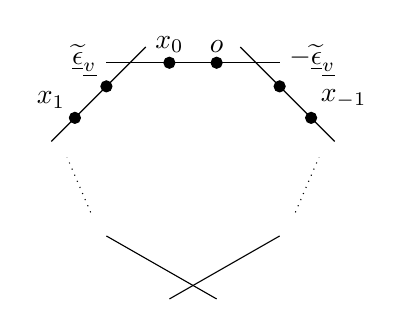
\begin{tikzpicture}
\draw (-0.3,0) -- (1.1,0.8);
\draw (0.3,0) -- (-1.1,0.8);
\draw (-1.8,2) -- (-0.6,3.2);
\draw (1.8,2) -- (0.6,3.2);
\draw (-1.1,3) -- (1.1, 3);
\draw[dotted]  (1.3, 1.1) -- (1.6, 1.8);
\draw[dotted]  (-1.3, 1.1) -- (-1.6, 1.8);
\filldraw[black] (-0.3, 3) circle (2pt); \node (x_0) at (-0.3, 3) [above] {$x_0$};
\filldraw[black] (0.3, 3) circle (2pt); \node (o) at (0.3, 3) [above] {$o$};
\filldraw[black] (-1.5, 2.3) circle (2pt); \node (xp) at (-1.5, 2.3) [above left] {$x_{1}$};
\filldraw[black] (-1.1, 2.7) circle (2pt); \node (pe) at (-1.1, 2.7) [above left] {$\widetilde{\uep}_{\uv}$};
\filldraw[black] (1.5, 2.3) circle (2pt); \node (xm) at (1.5, 2.3) [above right] {$x_{-1}$};
\filldraw[black] (1.1, 2.7) circle (2pt); \node (me) at (1.1, 2.7) [above right] {$-\widetilde{\uep}_{\uv}$};
\end{tikzpicture}
\caption{Special fiber of $\uX{}_{\uv}$}
\label{fig:SpecialFiberOfuuX}
\end{center}
\end{figure}

Figure \ref{fig:SpecialFiberOfuuX} illustrates the special fiber of $\uX{}_{\uv}$.
Here $o$ is the origin, $x_0$ is the unique nontrivial $2$-torsion point lying on the same component as $o$, and the $x_i$ are translates of $x_0$.
Note that the point $x_j$ is the image of the point $\xi_j\in \ddot{Y}_{\uv}$ defined in the preceding subsection.
The cusps $\pm \widetilde{\uep}_{\uv}$ are the cusps lying above the cusp $\uep_{\uv}$ of $\uC_{\uv}$.


\setcounter{equation}{0}
\section{Local GM-data and log-shells}
\subsection{Dismantling ring structures}\label{sub:dismantlingRingStr}
By Assumption \ref{assum:GaloisnessAssumption}, for two places $v_i$ ($i=1,2$) of $K$ whose restrictions to $F_{\tmod}$ coincide, the arithmetic geometries of the localizations of $X_F$ at the respective $v_i$ are mutually isomorphic.
Thus, intuitively, one is led to an idea of ``arithmetic geometry'' of the form in which one localizes objects over $K$ at the primes of $\uV$ and globalizes them using the product formula for $F_{\tmod}$.
Assumption \ref{assum:uXtopologicalOverX} assumes the existence of global data $(\alpha\colon\uX{}_K\to X_K,\uep)$ satisfying the local condition described above at each $\uv\in\uV^{\bad}$; this can be regarded as the existence of a GMS (cf.\ \S\ref{sub:GMS}) over ``$F_{\tmod}$ cut out inside $K$'' (or the image of a ``section'' of $\Spec K\to\Spec F_{\tmod}$\footnote{Such a non-scheme-theoretic section is represented by what Mochizuki calls a {\it prime-strip}, which we will also discuss later in \S\ref{sub:primeStrips}}).

As mentioned in \S\ref{sub:GMS}, the existence of such global data $(\alpha\colon\uX{}_K\to X_K,\uep)$ which satisfies the local condition for all $v\in \bV(K)^\bad$ is extremely rare, and this is what makes it difficult to prove the Szpiro conjecture for elliptic curves over number fields.
However, the existence of $(\alpha\colon\uX{}_K\to X_K,\uep)$ over ``$F_{\tmod}$ cut out inside $K$'' as above is not so rare.

IUT theory aims to prove the Szpiro conjecture from this setting, using this ``partial'' GMS.
However, to do so, one must isolate the ``$\uV$ part'' from the field $K$ and discuss it separately. 
Since $\uV$ is a subset of $\bV(K)$ that is neither finite nor cofinite, ``isolating'' just that part cannot be achieved using standard operations in arithmetic geometry. 
Mochizuki attempts to achieve this through a non-standard operation---one that involves ``dismantling the ring structure'':

\medskip
\begin{quote}
Thus, it is precisely by working with
such ``local analytic sections''---i.e., more concretely, by working
with the collection of valuations $\uV$, as opposed to the set of
{\it all} valuations of $K$---that one can, in some sense, {\it
``simulate''} the notions of a {\it ``global multiplicative
subspace''} or a {\it ``global canonical generator''}.  On the other
hand, such ``simulated global objects'' may only be achieved at the
cost of

\medskip
\begin{quote}
{\bf ``dismantling''}, or performing {\bf ``surgery''} on, the
{\it {\bf global prime structure} of the number fields} involved [...]
%[cf. the discussion of Remark \X{4.3.1}]
\end{quote}

\medskip
---a quite {\it drastic} operation, which has the effect of
precipitating {\it numerous technical difficulties}, [...] (\cite[Introduction, pp.\ 12--13]{MR4225473})
\end{quote}


\subsection{Mono-anabelian geometry}\label{sub:monoAnabelilanGeom}
As the following excerpt shows, Mochizuki believes that techniques from anabelian geometry, especially {\it absolute anabelian geometry} \cite{MR2987306,MR3154380,MR3445958}, is necessary to realize such a theory:

\medskip
\begin{quote}
This inter-universal
aspect of the theory manifestly leads to the issue of considering 

\medskip
\begin{quote}
the extent to which one can understand {\it various ring/scheme
structures} by considering only the underlying {\bf abstract
topological group} of some \'etale fundamental group arising from such 
a ring/scheme structure 
\end{quote}

\medskip
---i.e., in other words, of considering the {\bf absolute anabelian
geometry}[.] (\cite[\S I3, p.\ 26]{MR4225473})
\end{quote}

\medskip
Therefore, we need to briefly review the basics of anabelian geometry.
To begin with, the central theme of anabelian geometry lies in a ``reconstruction game'' in which, for example, one reconstructs objects such as algebraic number fields or hyperbolic curves solely from the topological group-theoretic structure of their arithmetic fundamental groups (Galois groups).

Traditionally, a theorem of anabelian geometry has asserted, for example, that for suitable varieties $X,Y$ over an algebraic number field $k$ (e.g., finite extensions of $k$, hyperbolic curves over $k$, and so on), the natural morphism
\begin{equation}\label{eqn:bi-anabelian}
\mathrm{Isom}_k(X,Y)\longto\mathrm{Isom}_{\GG_k}(\pi^{\et}_1(X),\pi^{\et}_1(Y))/\mathrm{Inn}(\pi^{\et}_1(\ovl{Y}))
\end{equation}
(where $\GG_k$ is the absolute Galois group $\Gal(\ovl{k}/k)$ of $k$, and $\ovl{Y}=Y\otimes_k\ovl{k}$) is a bijection.
A statement of this form prepares two objects, such as the above $X,Y$, and asks whether their ``comparison'' can be reconstructed from a comparison at the level of arithmetic fundamental groups.
By contrast, Mochizuki considered statements of the form in which $X$ itself is reconstructed directly from the arithmetic fundamental group $\pi^{\et}_1(X)$.
Since the former sort of statement treats the comparison of ``two'' objects, whereas the latter treats ``one'' object, Mochizuki calls the former {\it bi-anabelian geometry} and the latter {\it mono-anabelian geometry}\footnote{For a concise introduction to  mono-anabelian geometry, see, e.g., \cite{MR4491969}.}.

\subsection{Input objects for reconstruction algorithms}\label{sub:inputObjects}
In mono-anabelian geometry, the center of the substantive argument lies in the ``algorithm'' that reconstructs $X$ from the arithmetic fundamental group $\pi^{\et}_1(X)$.
For this reason, delicate aspects of the treatment of objects appear, for example, in the question of what sorts of objects are to be used as inputs of the algorithm.
As suggested by (\ref{eqn:bi-anabelian}), typically the input object is something like ``a surjective homomorphism of topological groups
\begin{equation}\label{eqn:typicalInputObject}
\pi^{\et}_1(X)\surjlongto \GG_k
\end{equation}
considered modulo inner automorphisms by its kernel,'' but a little tricky point here is that, despite the notation of (\ref{eqn:typicalInputObject}), these fundamental groups are treated as abstract topological groups and with allowance for indeterminacies arising from certain automorphisms.

Viewing a fundamental group as an abstract group means disregarding its action on the system of coverings, i.e., one has to discard the ``interpretation as a fundamental group.''
This distinction can be illustrated by a more elementary example as follows.

\begin{exa}\label{exa: symmetricGroup} 
The symmetric group $S_n$ of degree $n$ (where $n\geq 3$ to avoid trivial situations) is usually treated as the group of all bijections of the set $[n]=\{1,2,\ldots,n\}$ consisting of $n$ elements.
The difference from $S_n$ as an abstract group (i.e., ``$S_n$ without the interpretation as a permutation group'') lies in whether or not one considers the action $S_n\acton [n]$ at the same time.
For $S_n$ considered together with its action, there is no problem in defining, for example, the signature of an element $\sigma\in S_n$ and its cycle type.
But can similar concepts be defined for an element of an abstract group $G$ isomorphic to $S_n$?
This question asks whether these concepts can be defined solely from the group structure of $G$, not relying on the action.
There is no problem for the signature, since the commutator subgroup $D(G)$ of $G$ is always mapped onto $A_n$ by any group isomorphism $G\cong S_n$.
On the other hand, the cycle type can be reconstructed when $n\neq 6$, but not when $n=6$.
Indeed, if $n\neq 6$, every automorphism of $S_n$ is an inner automorphism and preserves conjugacy classes, and in this case, one can construct, from the abstract group $G$ alone, an $n$-point set $X(G)$ together with an action $G\acton X(G)$ such that any group isomorphism $G\cong S_n$ can be extended to an isomorphism (cf.\ \S\ref{subsub:morphismBetweenActions}) from the action $G\acton X(G)$ to the action $S_n\acton [n]$.
However, for $n=6$, such an action cannot be constructed (from the group structure of $G$ alone), since in this case there exists an automorphism of $S_6$ that sends transpositions to elements of cycle type $(2,2,2)$.
\end{exa}

\begin{rem}
With the above description, the issue is fundamentally related to whether or not $S_n$ is considered merely as a group, or as a group endowed with an action on $[n]$.
This has important \textit{practical} implications in terms of Lean formalization, primarily around the so-called \textit{typeclass system}.
The concrete spelling of $S_n$ in Mathlib usually has the spelling \texttt{Perm (Fin n)}, i.e.~the type of permutations of \texttt{Fin n}, which is the standard type with $n$ elements.
This type \texttt{Perm (Fin n)} comes endowed with two instances:
\begin{enumerate}
\item \texttt{Group (Perm (Fin n))} and
\item \texttt{MulAction (Perm (Fin n)) (Fin n)}.
\end{enumerate}
The first corresponds to the group structure on $S_n$, whereas the second corresponds to the action of $S_n$ on $[n]$.
Since these are both registered as instances, Lean's typeclass system will \textit{always} consider both when we write \texttt{Perm (Fin n)}.
In other words, Lean's typeclass system \textit{always} considers $S_n$ as being endowed with its action on $[n]$.

The process of passing from $S_n$ to $G$ also has a clear analogue in Lean.
That is, we can define a copy $G$ of $S_n$ as \texttt{def G (n\ :\ Nat)\ := Perm (Fin n)}, and endow it \textit{only} with the group structure as \texttt{instance (n\ :\ Nat)\ :\ Group (G n)\ := inferInstanceAs (Group (Perm (Fin n)))}.
If this is done, then we will be able to use Lean's typeclass system to see \texttt{G n} as a group, but \textit{not} as a group endowed with an action on $[n]$.
\end{rem}


\subsection{Coricity}\label{sub:coricity}
Techniques from mono-anabelian geometry play a decisive role in the ``method by links'' described in \S\ref{sub:methodByLink} and \S\ref{sub:HodgeTheaterThetaLink}. In this method, the calculation of the degrees of line bundles on both sides must be synchronized under the link \eqref{eqn:naiveLink} (i.e., where several ring-theoretic and scheme-theoretic structures cannot be shared). In other words, we must carry out ``the same task'' simultaneously using only the limited information that can be shared via links.

Therefore, when discussing in the situation like this, it is sometimes necessary to consider the question of what sort of structures are compatible with \eqref{eqn:naiveLink}.
This is a property often referred to as {\it coricity} in IUT theory. IUT theory encompasses various types of coricity concepts in different contexts. What we are discussing here as coricity is the one for properties and concepts that remain invariant under (various) links, as indicated in the following excerpt.

\medskip\noindent
\begin{quote}
So far, [...] we have
discussed various {\it ``coricity''} properties---i.e., properties
of {\it invariance} with respect to various types of
``transformations''---in the context of 
$\Th$-/$\Th^{\times\bmu}$-/$\Th^{\times\bmu}_{\text{gau}}$-/$\Th^{\times\bmu}_{\LGP}$-/$\Th^{\times\bmu}_{\mathfrak{lgp}}$-links, as
well as in the context of $\mathfrak{log}$-links. (\cite[Introduction, p.\ 408]{MR4225475})
\end{quote}

\medskip
Incidentally, in IUT theory, Mochizuki uses such a terminology as {\em (arithmetic) holomorphic} structure (AHS), which, according to our understanding, refers to the following kinds of concepts:
\begin{itemize}
    \item a ``ring-theoretic environment'' to which several ring-theoretic objects are associated;
    \item a structure that gives rise to a ``process to reconstruct'' the ring structure.
\end{itemize}
In opposition to this, a genuinely weaker underlying structure beneath a holomorphic structure is called a {\em mono-analytic} structure.

Although we generally would like to avoid using these somewhat ambiguous terms as much as possible, if we use them, one can express, by saying that ``AHS is not coric with respect to our link \eqref{eqn:naiveLink},'' the fact that the respective number fields ``$F$,'' their algebraic closures ``$\oF$'' and completions ``$F_v$,'' the algebraic closures ``$\oF_v$'' of the completions, the elliptic curves ``$E$'' and ``$E_v$,'' and the hyperbolic curves ``$X$'' and ``$X_v$,'' which belong to the two settings on the $\dag$-side and the $\ddag$-side, are all not coric under the link.
After all, since our link is not compatible with the ring structures, it is natural that rings and schemes cannot be shared on the two sides of our link.

\subsection{Coricity of local Galois groups}\label{sub:localGaloisGroup}
In this context, the first thing to notice is that there does not seem to be any circumstance that prevents the local Galois group $\GG_{\uv}$ from being coric with respect to the link (\ref{eqn:naiveLink}).
Indeed, the natural action of $\GG[\dag]_{\uv}$ (the $\GG_{\uv}$ on the $\dag$-side) on $\qq[\dag]_{\uv}^N$ and the natural action of $\GG[\ddag]_{\uv}$ (the $\GG_{\uv}$ on the $\ddag$-side) on $\qq[\ddag]_{\uv}$ are both trivial; hence, for any isomorphism of topological groups $\GG[\dag]_{\uv}\cong\GG[\ddag]_{\uv}$, (\ref{eqn:naiveLink}) is (trivially) equivariant.
That is to say, from the point of view of the topological group $\GG_{\uv}$, there is no great difference between $q_{\uv}^N$ and $q_{\uv}$.
Indeed, ``$\GG_{\uv}$'' is chosen, in the actual $\Th$-link in IUT theory, as an object to be shared, and hence is coric.

Importantly, also in this situation, in order to regard ``$\GG_{\uv}$'' as coric, one must discard the ``interpretation as a Galois group'' of them.
At the level of the definition, $\GG_{\uv}$ is defined as the group of suitable automorphisms of the field $\oF_{\uv}$.
Since the link under consideration is not compatible with ring structures, this sort of ``ring-theoretic interpretation'' of $\GG_{\uv}$ cannot be coric.
Consequently, an identification of $\GG[\dag]_{\uv}$ and $\GG[\ddag]_{\uv}$ that is compatible with the link becomes possible only after one regards each of them as an abstract topological group.

Thus, in particular, an identification $\GG[\dag]_{\uv}\simto\GG[\ddag]_{\uv}$ must take into consideration, as possibilities, {\it all isomorphisms} between these two topological groups.
Put another way, an identification across the link between $\GG[\dag]_{\uv}$ and $\GG[\ddag]_{\uv}$ requires one to consider the $\Aut(\GG[\dag]_{\uv}) \simeq \Aut(\GG[\ddag]_{\uv})$-orbit of an isomorphism $\GG[\dag]_{\uv}\simto\GG[\ddag]_{\uv}$.
To begin with, since $\GG[\dag]_{\uv}$ and $\GG[\ddag]_{\uv}$ are merely abstract topological groups, each belonging to a separate ring-theoretic environment, there is no canonical correct answer for an identification between them.
Therefore, we have no choice but to adopt the standpoint of constructing a theory in which no problem arises no matter which identification $\GG[\dag]_{\uv}\simto\GG[\ddag]_{\uv}$ is adopted.
This is one of the points at which the ``approach by links'' adopted by IUT theory differs decisively from ordinary arithmetic geometry, and the mono-anabelian geometry plays a large role.

Let us now explain one more piece of terminology from IUT theory.
In IUT theory, for two objects $A,B$, a certain (usually nonempty) set of morphisms from $A$ to $B$ is called a {\em poly-morphism}, a certain (usually nonempty) set of isomorphisms from $A$ to $B$ is called a {\em poly-isomorphism}, and the set of all isomorphisms from $A$ to $B$ is called the {\em full poly-isomorphism}.
Using this terminology, the conclusion of the discussion above may be phrased as follows: in order to identify the local Galois groups $\GG[\dag]_{\uv}$ and $\GG[\ddag]_{\uv}$ across our link, this identification should be the full poly-isomorphism.


\subsection{Coricity of local units}\label{sub:localUnits}
As observed above, data involving ring-theoretic structures are, in general, not coric with respect to the link \eqref{eqn:naiveLink}.
For example, one cannot share the field $\oK_{\uv}$ or the ring of integers $\oOO_{\uv}$, since the value groups are not coric with respect to the link.
For the same reason, the underlying multiplicative monoids $\oKx_{\uv}$ and $\oOOt_{\uv}$ cannot be coric either: indeed, their quotients by the group of units $\oOOx_{\uv}$ give the value group.

On the other hand, the group of units $\oOOx_{\uv}$, equipped with the canonical $\GG_{\uv}$-action, can be a coric object with respect to the link (\ref{eqn:naiveLink}).
However, in this case as well, just as in the case of $\GG_{\uv}$ discussed above, one must discard the provenance that ``$\oOOx_{\uv}$ was constructed as a subquotient of the field $\oK_{\uv}$'' and regard it as a ``bare'' topological $\GG_{\uv}$-module.
Here, this abstract pair $\GG_{\uv}\acton\oOOx_{\uv}$ carries a natural $\hbZ^{\times}$-symmetry, and this symmetry acts nontrivially on the cyclotomic portion
\[
\oOOmu_{\uv} \eqdef (\oOOx_{\uv})_{\tor} \subseteq \oOOx_{\uv}
\]
that arises from $\oOOx_{\uv}$.
As we shall see in \S\ref{sub:cyclotomicRigidity}, it is difficult to control the indeterminacy arising from this action (the ``indeterminacy with respect to cyclotomes'').

We therefore consider the mono-analytic object obtained as the quotient of $\oOOx_{\uv}$ by its cyclotomic portion $\oOOmu_{\uv} \subseteq \oOOx_{\uv}$:
\[
\GG_{\uv}\acton \oOOxmu_{\uv} \eqdef \oOOx_{\uv}/\oOOmu_{\uv}.
\]
This object is chosen, in the actual $\Th$-link in IUT theory, as an object to be shared, and hence is coric. In brief, it is a unit-group-like portion of $\oK_{\uv}$ that is isolated from the deformation of the value-group portion, and functions as a ``common container'' shared between the two Hodge Theaters.


\subsection{GM-data}\label{sub:GMdata}
The name {\it GM-data} ({\it group-monoid-pair} in \cite[Def.\ 5.1]{MR4491969}) refers to a type of data consisting of a group and a monoid as follows:
\begin{dfn}[{cf.\ \cite[Def.\ 5.1]{MR4491969}}]\label{dfn:GMdata}
A triple consisting of a topological group $G$, a topological monoid $M$, and a continuous group action
$$
G\acton M
$$
is called {\em GM-data}.
A morphism between GM-data $G\acton M$ and $G'\acton M'$ means a pair consisting of a homomorphism of topological groups $G\to G'$ and a homomorphism of topological monoids $M\to M'$ that gives a morphism of actions (cf.\ \S\ref{subsub:morphismBetweenActions}).
\end{dfn}

In GM-data $G\acton M$, the topological group $G$ is called its {\em \'etale-like portion}, and $M$ is called its {\em Frobenius-like portion}.

In IUT theory, one often considers abstract GM-data that are isomorphic to the GM-data
\begin{equation*}
\Pi_{\uv}\acton\oOOt_{\uv}\quad\text{or}\quad \GG_{\uv}\acton \oOOxmu_{\uv}.
\end{equation*}
Following the terminology of IUT theory, let us call the former {\em holomorphic GM-data} and the latter {\em mono-analytic GM-data}. These terms are used only provisionally in this manuscript.


\subsection{Notation for abstract copies}\label{sub:abstractCopies}

As mentioned earlier, the mathematical structures of a fundamental group and its abstract copy differ significantly. While IUT theory distinguishes these differences systematically to some extent through notation, it appears that the distinction is not fully captured by notation alone, and to some extent, it must be determined based on context.

\subsubsection{Fundamental/Galois groups}
With regard to fundamental groups, the following notation is used (to a certain extent) consistently (\cite[Def.\ 3.1(e), (f), p.\ 70--71]{MR4225473}):
\begin{itemize}
\item[(a)] $\GG_{\uv}$ denotes the local absolute Galois group $\Gal(\ovl{K}_{\uv}/K_{\uv})$.
\item[(b)] $\Pi_{\uv}$ denotes the following: 
\begin{itemize}
\item[(b1)] When $\uv\in\uV^{\bad}$, it denotes the tempered fundamental group $\pi_1^{\temp}(\uuX_{\uv})$;
\item[(b2)] When $\uv\in\uV^{\good}$, it denotes the {\'e}tale fundamental group $\pi^{\et}_1(\uaX_{\uv})$.
\end{itemize}
\end{itemize}

Note that, in either case, there exists a natural surjective homomorphism
$$
\Pi_{\uv}\surjlongto \GG_{\uv}.
$$

If these objects are marked with a superscript in the upper-left corner, such as $\GG[\dag]_{\uv}$ or $\PPi[\ddag]_{\uv}$, they are all considered to be isomorphic copies as abstract topological groups.
As noted in \S\ref{sub:inputObjects}, one must keep in mind that, a priori, copies ``come with no geometric interpretation at all as fundamental/Galois groups.''


\subsubsection{Labeling by indices}
As mentioned above, in IUT theory in general, multiple objects that are isomorphic each other are often labeled by left superscripts.
These may be labels of Hodge theaters, or they may be used as labels to distinguish such multiple objects when they are treated systematically in a given context of discussion.
For example, an object belonging to the Hodge theater at the coordinate $(m,n)$ of the log-theta-lattice or {\it big-H diagram} (cf.\ \S\ref{sub:BigHdiagram} below), or an object constructed from an object belonging to it by means of subquotients and the like, is written, for example, as
\begin{equation*}
  \GG[(m,n)]_{\uv}\acton \OOxmu[(m,n)]_{\uv}.
\end{equation*}
Moreover, when it is necessary in the context of discussion to distinguish objects by ad hoc labels, one writes, for example, using $\dag$ and $\ddag$,
\begin{equation*}
\GG[\dag]_{\uv}\acton\OOxmu[\dag]_{\uv},\quad \GG[\ddag]_{\uv}\acton\OOxmu[\ddag]_{\uv}
\end{equation*}
and so on (both of these are isomorphic to $\GG_{\uv}\acton\OOxmu_{\uv}$, but they are distinguished as objects with different labels).


\subsubsection{Monoids}
With regard to monoids such as $\oOOt_{\uv}$ and $\oOOxmu_{\uv}$, it does not seem that a precise distinction is made in the notation as to whether they are subquotients of the field $\oK_{\uv}$ fixed by the context, or whether they are isomorphic copies of them. Therefore, one must to some extent infer this from the context.

For example, when we say that we ``glue'' $\oOOxmu_{\uv}$—as an abstract monoid—to the Hodge theater $\HT[(m,n)]$, this means identifying it via a poly-isomorphism with $\oOOxmu[(m,n)]_{\oK_{\uv}}$, which is constructed as a subquotient of $\oK[(m,n)]_{\uv}$\footnote{Here we distinguished $\oOOxmu[(m,n)]_{\oK_{\uv}}$ from $\oOOxmu_{\uv}$ by notation, but we are not entirely sure whether this way of distinction is thoroughly consistent.}.


\subsection{Compact structure}\label{sub:cptStr}
When an object such as $\oOO_{\uv}$, $\oOOt_{\uv}$, or $\oOOx_{\uv}$ is given as an abstract ring or monoid, the version without an overline is defined by its $\GG_{\uv}$-invariant portion.
For example, when one is given a monoid that is isomorphic to the monoid $\oOOt_{\uv}$ (denoted by the same symbol), $\OOt_{\uv}$ is defined by
$$
\OOt_{\uv}\eqdef(\oOOt_{\uv})^{\GG_{\uv}}.
$$
Moreover, the version without an overline of $\oOOxmu_{\uv}$ is defined as the image of
$$
\OOx_{\uv}\eqdef(\oOOx_{\uv})^{\GG_{\uv}}\longto\oOOxmu_{\uv}.
$$


Here, we note that $\OOxmu_{\uv}$ cannot be determined from the abstract GM-data $\GG_{\uv}\acton \oOOxmu_{\uv}$ alone.
Therefore, for data of the form $\GG_{\uv}\acton \oOOxmu_{\uv}$, one often considers at the same time the following additional structure:
\begin{dfn}[$\xmu$-Kummer structure]\label{dfn:compactStructure}
For every open subgroup $H<\GG_{\uv}$ of $\GG_{\uv}$, define $\cI^{\kappa}_H$ to be the image of $(\oOOx_{\uv})^H$ under $\oOOx_{\uv}\surjto\oOOxmu_{\uv}$.
The resulting family
$$
\{\cI^{\kappa}_H\}_{H\overset{\text{open}}{<}\GG_{\uv}}
$$
is called the {\em $\xmu$-Kummer structure} or {\em compact structure} of $\GG_{\uv}\acton \oOOxmu_{\uv}$.
\end{dfn}

Mono-analytic GM-data equipped with compact structure is therefore a pair which is abstractly isomorphic to the pair
$$
(\GG_{\uv}\acton\oOOxmu_{\uv}, \{\cI^{\kappa}_H\}_H).
$$
In other words, it is a pair of the form $(G\acton M,\{N_H\}_H)$ where
\begin{itemize}
\item[(a)] $G\acton M$ is mono-analytic GM-data;
\item[(b)] $\{N_H\}_H$ is a family of submonoids of $M$ indexed by open subgroups $H<G$ of $G$ such that, for some isomorphism between $G\acton M$ and $\GG_{\uv}\acton \oOOxmu_{\uv}$, it corresponds to $\{\cI^{\kappa}_H\}_H$.
\end{itemize}

\subsection{Prime-strips}\label{sub:primeStrips}
In IUT theory, the local data
\[
\GG_{\uv},\quad \GG_{\uv} \acton \oOOx_{\uv},\quad
\bigl(\GG_{\uv} \acton \oOOxmu_{\uv},\{\cI^{\kappa}_H\}_H\bigr)
\]
are denoted by the symbols
\[
\cDv_{\uv},\quad \cFvx_{\uv},\quad \cFvxmu_{\uv}
\]
respectively.
Here, the superscript ``$\vdash$'' denotes ``mono-analytic''.
Also, the local data
\[
\Pi_{\uv},\quad \Pi_{\uv} \acton \oOOt_{\uv}
\]
are denoted by the symbols
\[
\cD_{\uv},\quad \cF_{\uv}
\]
respectively.
Here, $\Pi_{\uv} \acton \oOOt_{\uv}$ is the action determined by the natural surjection $\Pi_{\uv} \surjto \GG_{\uv}$ (constructed group-theoretically from $\Pi_{\uv}$).

\begin{rem}
More precisely, for example, the object denoted by the symbol $\cDv_{\uv}$ is not the profinite group $\GG_{\uv}$ itself. Rather, it is the full subcategory consisting of connected objects of the Galois category determined by this profinite group. From the general theory of Galois categories, the profinite group $\GG_{\uv}$ can be reconstructed from $\cDv_{\uv}$ up to inner automorphism. In this sense, $\GG_{\uv}$ and $\cDv_{\uv}$ are ``roughly equivalent data.''

Similarly, in the case of $\cFvx_{\uv}$, the object denoted by the symbol $\cFvx_{\uv}$ is not the GM-data $\GG_{\uv} \acton \oOOx_{\uv}$ itself. Rather, it is a certain Frobenioid whose data are equivalent to this GM-data.
\end{rem}

\renewcommand{\arraystretch}{1.3}
\begin{table}[ht]
    \centering
    \begin{tabular}{|c|c|}
        \hline
         Symbol & Data \\ \hline\hline
        $\cDv_{\uv}$ & $\GG_{\uv}$\\ \hline
        $\cFvx_{\uv}$ &  $\GG_{\uv} \acton \oOOx_{\uv}$\\ \hline
        $\cFvxmu_{\uv}$ & $\bigl(\GG_{\uv} \acton \oOOxmu_{\uv},\{\cI^{\kappa}_H\}_H\bigr)$\\ \hline
        $\cD_{\uv}$ &  $\Pi_{\uv}$\\ \hline
        $\cF_{\uv}$ & $\Pi_{\uv} \acton \oOOt_{\uv}$\\ \hline
    \end{tabular}

    \bigskip
    \caption{Local data}\label{tab: Local data}
\end{table}

These objects also have ``infinite-place versions.''  An object abstractly isomorphic to the collection of these local data, i.e.,
$$
\{\cDv_{\uv}\}_{\uv \in \uV}\quad\text{(resp.\ $\{\cFvx_{\uv}\}_{\uv \in \uV}$, $\{\cFvxmu_{\uv}\}_{\uv \in \uV}$, $\{\cD_{\uv}\}_{\uv \in \uV}$, $\{\cF_{\uv}\}_{\uv \in \uV}$)}
$$
is called a $\cDv$-\emph{prime-strip} (resp.\ $\cFvx$-\emph{prime-strip}, $\cFvxmu$-\emph{prime-strip}, $\cD$-\emph{prime-strip}, $\cF$-\emph{prime-strip}).


\setcounter{equation}{0}
\section{BPS and \'etale Hodge theater}\label{sec:BPSandEtHT}

\subsection{BPS}\label{sub:BPS}

In IUT theory, the $\Th$-link is constructed as an identification between data called $\cF^{\Vdash\blacktriangleright\times\bm{\mu}}$-prime-strips (cf.\ \cite[Def.\ 4.9, (viii), p.\ 384]{MR4225474}). In this report, we use a simplified notion, which we call a \emph{basic prime strip} (BPS), as a nearly equivalent substitute for this concept. A BPS consists of two portions: the \'etale-unit portion and the value-group portion.


\subsubsection{\'Etale-unit BPS}\label{subsub:etUnitBPS}
\begin{dfn}\label{dfn:etBPS}\ 

\begin{enumerate}
    \item An \emph{\'etale BPS} is a $\cDv$-prime strip, i.e., a collection
    $$
    \{\GG_{\uv}\}_{\uv\in\uV}
    $$
    indexed by $\uv\in\uV$ consisting of topological groups that are isomorphic to the local Galois group at $\uv$.
    \item An isomorphism of \'etale BPSs from $\{\GG_{\uv}\}_{\uv\in\uV}$ to $\{\GG'_{\uv}\}_{\uv\in\uV}$ is a collection of isomorphisms $\GG_{\uv}\simto \GG'_{\uv}$ of topological groups. 
\end{enumerate}
\end{dfn}

\begin{dfn}\label{dfn:etUnitBPS}\ 

\begin{enumerate}
    \item An \emph{\'etale-unit BPS} is an $\cFvxmu$-prime strip, i.e., a collection
    \begin{equation}\label{eqn:etUnitBPS}
        \{(\GG_{\uv}\acton M_{\uv},\{N_{\uv,H}\}_H)\}_{\uv\in\uV}
    \end{equation}
    indexed by $\uv\in\uV$ consisting of mono-analytic GM-data with compact structure (\S\ref{sub:cptStr}); in other words, it is an object abstractly isomorphic to $\{(\GG_{\uv}\acton\oOOxmu_{\uv},\ \{\cI^{\kappa}_H\}_H)\}_{\uv\in\uV}$.
    \item An isomorphism of \'etale-unit BPSs from $\{(\GG_{\uv}\acton M_{\uv},\{N_{\uv,H}\}_H)\}_{\uv\in\uV}$ to $\{(G'_{\uv}\acton M'_{\uv},\{N'_{\uv,H}\}_H)\}_{\uv\in\uV}$ is a collection of isomorphisms $\{\phi_{\uv}=(\phi_{G,\uv},\phi_{M,\uv})\}$ from $\GG_{\uv}\acton M_{\uv}$ to $G'_{\uv}\acton M'_{\uv}$ (cf.\ \S\ref{subsub:morphismBetweenActions}) such that $\phi_{M,\uv}(N_{\uv,H})=N'_{\uv,\phi_{G,\uv}(H)}$.
\end{enumerate}

Note that one can reconstruct an \'etale-unit BPS from an \'etale BPS by a certain anabelian reconstruction algorithm.  
\end{dfn}

In the \'etale-unit BPS (\ref{eqn:etUnitBPS}), $\{\GG_{\uv}\}_{\uv\in\uV}$ is called the {\it \'etale portion}, which itself forms an \'etale BPS.  
Note that each isomorphism of \'etale-unit BPSs induces an isomorphism between their \'etale portions. 

\subsubsection{Value-group BPS}\label{subsub:valBPS}

\begin{dfn}\label{dfn:valBPS}
A \emph{value-group BPS} is a pair 
\begin{equation}\label{eqn:valBPS}
(\cC,\{\varphi_{\uv}\}_{\uv\in\uV})
\end{equation}
that consists of the data 
\begin{itemize}
\item[$\bullet$] a one-dimensional oriented $\bR$-vector space $\cC$; 
\item[$\bullet$] a collection of nonzero elements $\{\varphi_{\uv}\in \cC\}_{\uv\in\uV}$, called the \emph{local pilots}; 
\end{itemize}
such that $\varphi_{\cC} \eqdef \sum_{\uv\in\uV^{\bad}}\varphi{}_{\uv} \in \cC$ is nonzero.  
We shall refer to this sum $\varphi_{\cC} \eqdef \sum_{\uv\in\uV^{\bad}}\varphi{}_{\uv} \in \cC$ as a \emph{pilot} of the value-group BPS $(\cC,\{\varphi_{\uv}\}_{\uv\in\uV})$.  
\end{dfn}

Let $\cB$ be a value-group BPS as in (\ref{eqn:valBPS}).
Then it is immediate that the $\bR$-linear map
\begin{equation}\label{eqn:productFormula}
\bigoplus_{\uv\in\uV}\bR_{\uv}\longto\cC,
\end{equation}
where $\bR_{\uv}$ is a copy of $\bR$ for each $\uv\in\uV$, and the $\uv$-component $\bR_{\uv} \to \cC$ of this map is given by mapping $a \in \bR_{\uv}$ to $a\cdot \varphi_{\uv} \in \cC$, is surjective.  The kernel of this map is said to be the \emph{product formula} of $\cB$, denoted by $\PF(\cB)$.

\begin{dfn}\label{dfn:isoValBPSs}
Let $\cB=(\cC,\{\varphi_{\uv}\}_{\uv})$ and $\cB'=(\cC',\{\varphi'_{\uv}\}_{\uv})$ be two value-group BPSs.
An isomorphism $\Phi\colon\cB\simto\cB'$ of value-group BPSs is an $\bR$-linear isomorphism $
\cC\simto\cC'$ that maps $\varphi_{\uv} \in \cC$ to $\varphi'_{\uv} \in \cC'$ for every $\uv$.  
\end{dfn}

\begin{rem}\label{rem:definingValueGroupBPS}
The value-group BPSs that appear in the following discussion all have the same product formula $\PF\subset\bigoplus\limits_{\uv\in\uV}\bR_{\uv}$. In such a situation where the product formula is fixed, scaling the local pilots $\{\varphi_{\uv}\}_{\uv\in\uV}$ uniformly by a non-zero real number does not change the product formula; therefore, a value-group BPS is simply given by 
\begin{itemize}
\item a one-dimensional oriented $\bR$-vector space $\cC$;
\item a negative element $\varphi_{\cC}\in\cC$, called the \emph{pilot}.
\end{itemize}
In what follows, we will define value-group BPS in this form, i.e., a ``pointed oriented real line.''
\end{rem}


\subsubsection{BPS}\label{subsub:BPS}
\begin{dfn}\label{dfn:BPS}
(1) A \emph{basic prime strip} (BPS) $\cB$ is a pair
$$
\cB=(\cB^{\text{\'et-unit}},\cB^{\text{val}})
$$
of an \'etale-unit BPS and a value-group BPS.
By the \emph{pilot} of a BPS we mean the pilot of its value-group portion.

(2) An isomorphism of BPSs is a pair consisting of an isomorphism of the \'etale-unit portions and an isomorphism of the value-group portions.
\end{dfn}


\begin{lem}\label{lem:isomBPS}
Two BPSs $\cB=(\{\GG_{\uv}\acton M_{\uv},\{N_{\uv,H}\}_H\}_{\uv\in\uV},\cC,\{\varphi_{\uv}\}_{\uv\in\uV})$ and $\cB'=(\{G'_{\uv}\acton M'_{\uv},\{N'_{\uv,H}\}_H\}_{\uv\in\uV},\cC',\{\varphi'_{\uv}\}_{\uv\in\uV})$ are isomorphic to each other if and only if $\PF(\cB)=\PF(\cB')$.
\end{lem}

\begin{proof}
First, observe that we always have an isomorphism of the \'etale-unit portions.  Let $\Phi\colon(\cC,\{\varphi_{\uv}\}_{\uv})\simto (\cC',\{\varphi'_{\uv}\}_{\uv})$ be an isomorphism of value-group BPSs.
This means that the following diagram of $\bR$-vector spaces and $\bR$-linear homomorphisms is commutative:
$$
\xymatrix@C+3ex{
\bigoplus\limits_{\uv\in\uV}\bR_{\uv}\ar[r]^-{\varphi_{\cC}}\ar@{=}[d]&\cC\ar[d]_-{\wr}^-{\Phi}\\
\bigoplus\limits_{\uv\in\uV}\bR_{\uv}\ar[r]_-{\varphi_{\cC'}}&\cC'.
}
$$
Here, the horizontal arrows are the $\bR$-linear homomorphisms of \eqref{eqn:productFormula} for the value-group BPSs $\cB,\cB'$, respectively.  Then it is immediate that $\operatorname{Ker} \varphi_{\cC}=\operatorname{Ker} \varphi_{\cC'}$, i.e., $\PF(\cB)=\PF(\cB')$.
Conversely, if $\PF(\cB)=\PF(\cB')$, then there exists an $\bR$-linear isomorphism $\Phi\colon \cC\to \cC'$ which makes the above diagram commutative.  
\end{proof}


\subsection{\'Etale Hodge theater and $q$-pilot BPSs}\label{sub:EtHT}

\subsubsection{Hodge theaters and their \'etale-like portions}\label{subsub:HT}
As discussed in \S\ref{sub:HodgeTheaterThetaLink}, a link such as (\ref{eqn:naiveLink}) should be regarded as a relationship between ``environments,'' and the {\it Hodge theater} is such an environment. 
The first paper on IUT theory \cite{MR4225473} is devoted to the introduction of Hodge theaters.

In the usual setting of arithmetic geometry, the additive and multiplicative structures of number fields and local fields, the unit groups and the value groups, Galois actions, fundamental groups, and so on are intricately bound together.
For the reasons we have seen in \S\ref{sub:dismantlingRingStr}, the IUT theory ``unties'' this binding, and try to manage which information can be reconstructed from Galois groups or fundamental groups by anabelian geometry, and which information can be ``shared'' through a link.
From this, the Hodge theater is conceived as a ``stage'' for ordinary arithmetic geometry\footnote{
The following excerpt may explain the name ``Hodge'' theater: 
\begin{quote}
the position occupied by a {\it ``Hodge theater''} within [...]
the {\it ``log-theta-lattice''} [...]
corresponds precisely to the {\bf specification of a particular arithmetic
holomorphic structure} [...] (\cite[Introduction, p.\ 25]{MR4225473})
\end{quote}}.

Roughly speaking, a Hodge theater consists of many pieces of GM-data together with the relations among them.
In this report, we call the underlying structure of a Hodge theater obtained by considering only the \'etale-like portions of these pieces of GM-data an \emph{\'etale Hodge theater}. In the original papers, this is called a $\mathcal{D}$-$\Th^{\pm \mathrm{ell}}\mathrm{NF}$-Hodge theater.

An \'etale Hodge theater is roughly a system consisting of (topological groups isomorphic to) various \'etale/tempered fundamental groups, together with homomorphisms among them. Its components include the following: %}
\begin{enumerate}
\item[(1)] the \'etale fundamental groups $\pi_1^{\et}(\underline{C}{}_K)$, $\pi_1^{\et}(\underline{X}{}_K)$ of global hyperbolic orbicurves $\underline{C}{}_K$, $\underline{X}{}_K$; 
\item[(2)] at bad places, the tempered fundamental groups of local curves such as \(\Pi_{\uv}=\Pi^{\tp}_{\uuX_{\uv}}\), and their profinite completions.  
\end{enumerate}

In the sequel, for a Hodge theater $\HT$, its \'etale-like portion will be denoted by $\HT^{\cD}$, as the symbol $\cD$ often indices \'etale-like portion in the IUT theory.


\subsubsection{Objects that can be reconstructed from \'etale Hodge theater}\label{subsub:ObjectsReconstFromEtHT}
Let us recall (\cite[Prop.\ 1.2(vi)--(ix)]{MR4225475} and \cite[Prop.\ 3.2; Prop.\ 3.3]{MR3445958}) that one can reconstruct the following objects from (a topological group abstractly isomorphic to) the absolute Galois group $\GG_{\uv}$ by the relevant local mono-anabelian reconstruction algorithms, with local class field theory as one of the ingredients:  
\begin{itemize}
\item 
The residue characteristic $p = p_{\uv}$ of the local field $K{}_{\uv}$.  

\item 
The extension degree $d_{\uv}$ of the finite field extension $K{}_{\uv} / \mathbb{Q}_p$.  

\item 
The absolute ramification index $e_{\uv}$ of the local field $K{}_{\uv}$.  

\item 
The absolute residue degree $f_{\uv}$ of the local field $K{}_{\uv}$.  

\item 
The topological monoids $\oOOmu_{\uv} \subseteq \oOOx_{\uv} \subseteq \oOOt_{\uv}$ with the natural continuous actions of $\GG_{\uv}$.  

\item
The cyclotome (cf.\ \S\ref{subsub:cyclotomes})
\[
  \Lambda(\oOOx_{\uv})
  \eqdef
  \varprojlim_n (\oOOx_{\uv})^{\gp}[n].
\]

\end{itemize}
Let us also recall (\cite[Thm.\ 1.6; Thm.\ 1.10; Cor.\ 2.18; Cor.\ 2.19]{MR2512782} and \cite[Prop.\ 1.4]{MR4225474}) that one can reconstruct the following objects from (a topological group abstractly isomorphic to) the tempered fundamental group $\Pi_{\uv}$:  
\begin{itemize}
\item 
The topological field $\oK_{\uv}$ with the natural continuous action of $\Pi_{\uv}$.  

\item 
The embedding $K{}_{\uv}^{\times} = (\oKx_{\uv})^{\GG_{\uv}} \injto H^1(\Pi_{\uv}, \Lambda(\oOOx_{\uv}))$ by Kummer theory.  

\item 
At a bad place $\uv$, the $q$-parameter $q_{\uv} \in K{}_{\uv}^{\times}$ $(\subseteq H^1(\Pi_{\uv}, \Lambda(\oOOx_{\uv})))$ of the elliptic curve $E_{\uv}$ over $K{}_{\uv}$. 
\end{itemize}


\subsubsection{The $q$-pilot BPS}\label{subsub:qPilotBPS}
Let us fix a single \'etale Hodge theater $H$ and work inside it.
Due to what we have seen in \S\ref{subsub:ObjectsReconstFromEtHT}, one can construct an \'etale-unit BPS $B(H)$ from the objects that is reconstructed from $H$.

For each $\uv\in\uV^{\bad}$, let us write one of the $2l$-th roots of $q_{\uv}$ introduced in \S\ref{sub:SzpiroConjecture} as
$$
\uuqq_{\uv}.  
$$
For an element $a \in \OO_{F_v}$, we define 
$$
\deg(a) \eqdef [F:\bQ]^{-1}\log\bigl(\#(\OO_{F_v}/a\OO_{F_v})\bigr).
$$
Using this, one can construct a value-group BPS as follows:
\begin{itemize}
\item put $\cC\eqdef\bR$;
\item for each $\uv\in\uV$, define the local pilot $\varphi_{\uv} \in \cC$ at $\uv$ by
$$
\varphi_{\uv}=\begin{cases}\deg(\uuqq_{\uv}) & (\uv\in\uV^{\bad});\\ \deg(p_{\uv}) & (\uv\in\uV^{\good}\cap\uV^{\non});\\ 2\pi & (\uv\in\uV^{\arc}).\end{cases}
$$
\end{itemize}

The value-group BPS obtained in this way is called the \emph{$q$-pilot value-group BPS} in the \'etale Hodge theater $H$, and a BPS having this type of value-group portion is called a \emph{$q$-pilot BPS}.


\setcounter{equation}{0}
\section{Volume container and log-links}
\subsection{Log-shells}\label{sub:logShell}

As explained above, the main goal of IUT theory is to estimate the degrees of arithmetic line bundles. However, the integral structure $\OO_{\uv}\subset K_{\uv}$ needed in order to handle arithmetic line bundles is a holomorphic structure that cannot be shared via the $\Th$-link. The notion of a log-shell introduced in this section is an integral structure that serves as a substitute for $\OO_{\uv}$ for such a situation.

Let $\uv\in \uV^\non$. Then the $p$-adic logarithm map gives an isomorphism of groups
\[
\log\colon \oOOxmu_{\uv}\simlongto \oK_{\uv}.
\]
Using this, we define a $\bZ_p$-module $\LS_{\uv}$, called the \emph{log-shell} at $\uv$, by
\[
\LS_{\uv}=(2p_{\uv})^{-1}\cdot \Image (\OOx_{\uv}\hookrightarrow \oOOx_{\uv}\twoheadrightarrow \oOOxmu_{\uv}\xrightarrow{\log} \oK_{\uv})\subset K_{\uv};
\]
note that the factor $(2p_{\uv})^{-1}$ makes the inclusion $\OO_{\uv}\subset \LS_{\uv}$ to hold.
This construction of log-shells involves the function $\log$, whose formation requires the ``ring structure'' (i.e., addition and multiplication) on $\oOOxmu_{\uv}$.
But there are several different ways to construct log-shells, which we now explain. 


\subsubsection{Holomorphic Frobenius-like version (HF)}\label{subsub:HF}
This version of the log-shell is constructed from an $\cF$-prime strip (cf. \S\ref{sub:primeStrips})
$$
\cF=\{\Pi_{\uv}(\cF)\acton\oOOt_{\uv}(\cF)\}_{\uv\in \uV}.
$$
From the monoid $\oOOt_{\uv}(\cF)$, we construct the set $\oOOx_{\uv}(\cF)$ of invertible elements, the set $\oOOmu_{\uv}(\cF)$ of torsion elements, and the quotient $\oOOxmu_{\uv}(\cF)=\oOOx_{\uv}(\cF)/\oOOmu_{\uv}(\cF)$.
From the given action $\Pi_{\uv}(\cF)\acton\oOOt_{\uv}(\cF)$ one can construct (\cite[Prop.\ 3.2(iii),(v)]{MR3445958}) the ``new multiplication'' on $\oOOxmu_{\uv}(\cF)$ so that, with the original monoid multiplication regarded as the ``new addition,'' it becomes a field isomorphic to $\oK_{\uv}$ on which $\Pi_{\uv}$ acts.
Let us denote the field (acted on by $\Pi_{\uv}$) thus obtained by $\oK_{\uv}(\log\cF)$.
The \emph{holomorphic Frobenius-like log-shell} at $\uv$ associated to $\cF$ is a $\bZ_{p_{\uv}}$-submodule of $\oK_{\uv}(\log\cF)$ defined as
$$
\LS_{\uv}(\cF)=(2p_{\uv})^{-1}\cdot\Image(\OOx_{\uv}(\cF)\injto\oOOx_{\uv}(\cF)\surjto\oK_{\uv}(\log\cF)),
$$
where $\OOx_{\uv}(\cF)=(\oOOx_{\uv}(\cF))^{\Pi_{\uv}(\cF)}$.

\subsubsection{Holomorphic \'etale-like version (HE)}\label{subsub:HE}
This version of the log-shell is constructed from a $\cD$-prime strip (cf. \S\ref{sub:primeStrips})
$$
\cD=\{\Pi_{\uv}(\cD)\}_{\uv\in \uV}.
$$
From the topological group $\Pi_{\uv}(\cD)$, we can construct GM-data $\GG_{\uv}(\cD)\acton\oOOt_{\uv}(\cD)$ isomorphic to $\GG_{\uv}\acton\oOOt_{\uv}$ by an anabelian algorithm.
Similarly to what we did in (HF), we can construct $\Pi_{\uv}(\cD)\acton\oOOxmu_{\uv}(\cD)$ and $\oK_{\uv}(\log\cD)$.
The \emph{holomorphic \'etale-like log-shell} at $\uv$ associated to $\cD$ is a $\bZ_{p_{\uv}}$-submodule of $\oK_{\uv}(\log\cD)$ defined as
$$
\LS_{\uv}(\cD)=(2p_{\uv})^{-1}\cdot\Image(\OOx_{\uv}(\cD)\injto\oOOx_{\uv}(\cD)\surjto\oK_{\uv}(\log\cD)),
$$
where $\OOx_{\uv}(\cD)=(\oOOx_{\uv}(\cD))^{\Pi_{\uv}(\cD)}$.


\subsubsection{Mono-analytic Frobenius-like version (MF)}\label{subsub:MF}
This version of the log-shell is constructed from an $\cFvxmu$-prime strip (cf. \S\ref{sub:primeStrips})
$$
\{\GG_{\uv}\acton\oOOxmu_{\uv},\ \{\LS^{\kappa}_H\}_H\}_{\uv\in \uV}.
$$
The group $\oOOxmu_{\uv}$ is isomorphic to the underlying additive group of the field $\oK_{\uv}$.
The \emph{mono-analytic Frobenius-like log-shell} at $\uv$ is a $\bZ_{p_{\uv}}$-submodule of $\oOOxmu_{\uv}$ defined as
$$
\LS_{\uv}(\cFvxmu)=(2p_{\uv})^{-1}\cdot\Image(\LS^{\kappa}_{\GG_{\uv}}\injto\oOOxmu_{\uv}).
$$

\subsubsection{Mono-analytic \'etale-like version (ME)}\label{subsub:ME}
This version of the log-shell is constructed from a $\cDv$-prime strip (cf. \S\ref{sub:primeStrips})
$$
\{\GG_{\uv}\}_{\uv\in \uV}.
$$
One can construct via an anabelian algorithm an \'etale-like version $\oOOxmu_{\uv}(\GG_{\uv})$ of $\oOOxmu_{\uv}$ together with a compact structure $\{\LS^\kappa_H(\GG_{\uv})\}_H$.
The \emph{mono-analytic \'etale-like log-shell} at $\uv$ is a $\bZ_{p_{\uv}}$-submodule of $\oOOxmu_{\uv}(\GG_{\uv})$ defined as
$$
\LS_{\uv}(\cDv)=(2p_{\uv})^{-1}\cdot\Image(\LS^\kappa_{\GG_{\uv}}(\GG_{\uv})\injto\oOOxmu_{\uv}(\GG_{\uv})).
$$


\subsubsection{The roles of the four types of log-shells}\label{subsub:fourLogShellRoles}
According to Mochizuki, the four types of log-shells listed above each have their own roles. Following the description in the original IUT paper, let us organize them into a bulleted list.

\begin{itemize}
\item The \emph{holomorphic Frobenius-like} log-shells are constructed within a fixed arithmetic holomorphic structure and are essentially identical to the construction using the function $\log$ presented at the beginning of this section.
The \emph{holomorphic {\'e}tale-like} log-shell is used to introduce the ``upper semi-compatibility,'' which will be discussed later in \S\ref{subsub:upperSemiComp}; see \cite[Rem.~1.2.2(iii), pp.\ 442--443; Prop.~3.5(ii), pp. 517--520]{MR4225475}. In the notation of Theorem 3.11, this phenomenon is recorded as the third indeterminacy \(\IndThree\) \cite[Thm.\ 3.11(ii), pp. 577]{MR4225475}.

\item The \emph{mono-analytic Frobenius-like} log-shell and the \emph{mono-analytic {\'e}tale-like} log-shells are said to serve as containers for shaping the outputs of the multiradial algorithm (\S\ref{sec:multiradialThetaCor312}) and for transporting them between different Hodge theaters via $\Th$-links in situations where a complete ring-theoretic structure does not exist in the background; see \cite[Thm.~1.5(iii),(iv), pp.\ 455--457]{MR4225475} and \cite[Rem.~1.5.2(i), pp.\ 460--461]{MR4225475}. 
\end{itemize}

\subsection{Volume container}\label{sub:valueContainer}

As terminology used only in this exposition, we call the direct product $\prod_{\uv\in\uV} K_{\uv}$ of local fields the \emph{small volume container}. Each component $K_{\uv}$ of this direct product is called a \emph{small local volume container}. These serve as “containers” when arithmetic line bundles are represented by fractional ideals. Here, we introduce several variants of these notions.

\subsubsection{Large volume containers}\label{subsub:largeAndSmallVC}
Let $\ell$ be the prime number in the initial $\Th$-data. Set
\begin{itemize}
    \item $J=\mathbb{F}_{\ell}/\mathord{\pm} 1=\{0,1,2,\ldots,\ell^{\divideontimes}=\frac{\ell-1}{2}\}$;
    \item $S_j=\{0,1,\ldots,j-1\}$ for $j=1,2,\ldots,\ell^{\divideontimes}+1$.
\end{itemize}
The \emph{(large) local volume container} over $K$ at $\uv\in\uV$ is defined by
$$
\LocVC(K)_{\uv}=\bigoplus_{j\in J} K_{S_{j+1},\uv},
$$
where 
\[
K_{S_{j+1},\uv}=\bigl(\bigotimes_{t\in S_j}\bigoplus_{\underline{w}\mid \uv_\mathbb{Q}}K_{t,\underline{w}}\bigr)\otimes K_{j,\uv}.
\]
Here, $K_t$ are copies of $K$, $\uv_{\bQ}$ denotes the place of $\bQ$ that lies below $\uv$, and $\otimes=\otimes_{\mathbb{Q}_{\uv_{\mathbb{Q}}}}$.
The \emph{(large) volume container} over $K$ is defined as the product
$$
\VC(K)=\prod_{\uv\in\udl{\mathbb{V}}}\LocVC(K)_{\uv}.
$$

\subsubsection{Log-shell version}
The ``\emph{$\cI$-version}'' (``\emph{log-shell version}'') of the \emph{(large) volume container} (resp.\ \emph{(large) local volume container}), denoted by 
$$
\VC(\cI)\quad \text{(resp.\ $\LocVC(\cI)_{\uv}$),}
$$
is similarly defined, where $K_{\uv}$ is replaced by $\cI_{\uv}$ and $\otimes_{\bQ_{\uv_{\bQ}}}$ by $\otimes_{\bZ_{\uv_{\bQ}}}$.


\subsubsection{$\OO$-version}
The ``\emph{$\OO$-version}'' of the \emph{(large) local volume container}, denoted by
$$
\LocVC(\OO)_{\uv},
$$
is defined as follows:
$\LocVC(K)_{\uv}$ can be written as the direct sum of finitely many copies of $K_{\udl{w}}$, where $\udl{w}$ are places of $K$ that divides $\uv_{\bQ}$. Then $\LocVC(\OO)_{\uv}$ is obtained by replacing all $K_{\udl{w}}$ that appears in the direct sum decomposition by $\OO_{K_{\udl{w}}}$.
Equivalently, it is obtained by replacing $K_{\uv}$ by $\OO_{\uv}$ and $\otimes_{\bQ_{\uv_{\bQ}}}$ by $\otimes_{\bZ_{\uv_{\bQ}}}$ in the definition of $\LocVC(K)_{\uv}$, and then taking the integral closure.

The ``\emph{$\OO$-version}'' of the \emph{(large) volume container} is defined as the product
$$
\VC(\OO)=\prod_{\uv\in \uV}\LocVC(\OO)_{\uv}.
$$

\subsubsection{Holomorphic hull}
Note that $\VC(K)$ is naturally a $\VC(\OO)$-module.
For a subset $S\subset\VC(K)$, the \emph{holomorphic hull} of $S$, denoted by $S^{\hol}$, is the smallest $\VC(\OO)$-submodule of $\VC(K)$ that contains $S$. 

\subsubsection{Procession-normalized volume}\label{subsub:procNormLogVol}
One has the notion of ``\emph{volume}'' by Haar measure for measurable subsets in $\VC(K)$, which is normalized as: the volume of $\VC(\OO)$ is $1$, and multiplication by $p_{\uv}$ at $\uv$ acts as multiplication by $p_{\uv}^{-1}$ on the volume. 
For a measurable subset $S$ of $\VC(\OO)$, we denote $\logvol(S)$ the logarithm of the volume $\vol(S)$ (the \emph{log volume} of $S$).
For example, the log volume of $p_{\uv}\cdot\VC(\OO)$ (the multiplication being as above) is equal to $-\log (p_{\uv})$.

\begin{rem}
The above normalization implements what is called ``\emph{procession-normalization}'' in the original IUT papers.
\end{rem}


\subsubsection{The LGP element}\label{subsub:LGP}
We define the {\it LGP element} \footnote{In IUT papers, LGP stands for ``Logarithmic Gaussian Procession,'' which means a certain collection of the special values of the ``$l$-th root of the theta function'' of the form $\uuqq^{j^2}_{\uv}$ for $j=1,\ldots,l^{\divideontimes}$.} $\LGP\in\VC(\OO)$ as follows.
First, 
$$
\LGP=(\LGP_{\uv})_{\uv\in \uV},
$$
and $\LGP_{\uv}\in\LocVC(\OO)_{\uv}$ is further decomposed as
$$
\LGP_{\uv}=(\LGP_{S_{j+1},\uv})_{j\in J}\quad(\LGP_{S_{j+1},\uv}\in K_{S_{j+1},\uv}).
$$
Now, as an element in $K_{S_{j+1},\uv}=\bigl(\bigotimes_{t\in S_j}\bigoplus_{\underline{w}\mid \uv_\mathbb{Q}}K_{t,\underline{w}}\bigr)\otimes K_{j,\uv}$, 
$$
\LGP_{S_{j+1},\uv}=\begin{cases}
    (\bigotimes_{t\in S_j}(1)_{\udl{w}|\uv_{\bQ}})\otimes \uuqq^{j^2}_{\uv}&\text{if $\uv$ is bad,}\\
    (\bigotimes_{t\in S_j}(1)_{\udl{w}|\uv_{\bQ}})\otimes 1&\text{if $\uv$ is good.}
\end{cases}
$$


\subsection{log-links and log sequence}\label{sub:logLink}
\subsubsection{Log-link}\label{subsub:logLink}
Consider two copies of Hodge theaters $\HT[\dag]$ and $\HT[\ddag]$.
In $\HT[\dag]$ (resp.\ $\HT[\ddag]$), as in \S\ref{subsub:HF}, one has the two copies $\oK[\dag]_{\uv}$ ($=\oK[\dag]_{\uv}(\cF)$) and $\oK[\dag]_{\uv}(\log\cF)$ (resp.\ $\oK[\ddag]_{\uv}$ ($=\oK[\ddag]_{\uv}(\cF)$) and $\oK[\ddag]_{\uv}(\log\cF)$) of the field $\oK_{\uv}$.

We fix an isomorphism $\HT[\dag]^{\cD}\simto\HT[\ddag]^{\cD}$ between the \'etale-like portions of the Hodge theaters once for all. 
Then by the fact (\cite[Cor.\ 5.3 (ii), p.\ 160]{MR4225473}) that any isomorphism of $\cD$-prime strips can be uniquely lifted to an isomorphism of $\cF$-prime strips, one obtains a unique lift
$$
\log\colon\oK[\dag]_{\uv}(\log\cF)\simlongto\oK[\ddag]_{\uv}.
$$
We call this isomorphism a \emph{log-link} from $\HT[\dag]$ to $\HT[\ddag]$ (see Figure \ref{fig:LogLink}):
$$
\log\colon\HT[\dag]\longto\HT[\ddag].
$$

\begin{figure}[htbp]
$$
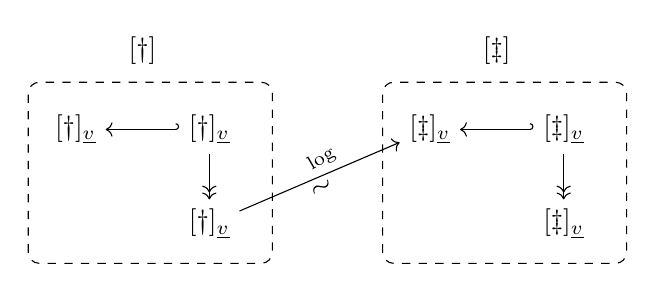
\begin{tikzpicture}
\coordinate (a) at (0,0);
\node (-1k) at ([shift={(0,1.2)}]a) {$\oK[\dag]_{\uv}$};
\node (-1Ox) at ([shift={(1.7,1.2)}]a) {$\oOOx[\dag]_{\uv}$};
\node (-1Oxmu) at ([shift={(1.7,0)}]a) {$\oOOxmu[\dag]_{\uv}$};
\draw[{Hooks[left]}->] (-1Ox) --(-1k);
\draw[->>] (-1Ox) --(-1Oxmu);
\draw[dashed, rounded corners] ([shift={(-.6,-.5)}]a) rectangle([shift={(2.5, 1.8)}]a);
\node at ([shift={(0.85,2.2)}]a) {$\HT[\dag]$};
%
\coordinate (a) at (4.5,0);
\node (0k) at ([shift={(0,1.2)}]a) {$\oK[\ddag]_{\uv}$};
\node (0Ox) at ([shift={(1.7,1.2)}]a) {$\oOOx[\ddag]_{\uv}$};
\node (0Oxmu) at ([shift={(1.7,0)}]a) {$\oOOxmu[\ddag]_{\uv}$};
\draw[{Hooks[left]}->] (0Ox) --(0k);
\draw[->>] (0Ox) --(0Oxmu);
\draw[dashed, rounded corners] ([shift={(-.6,-.5)}]a) rectangle([shift={(2.5, 1.8)}]a);
\node at ([shift={(0.85,2.2)}]a) {$\HT[\ddag]$};
\draw[->] (-1Oxmu) -- node[auto, rotate=30, pos=0.7]{$\scriptstyle \log$} node[auto=right, rotate=30, pos=0.36]{$\sim$} (0k);
\end{tikzpicture}
$$
\caption{The log-link}
\label{fig:LogLink}
\end{figure}

\begin{rem}\label{rem:underlyingBHT}
Since the \'etale-like log-shells $\LS[\et]$ and $\LS[\Gal]$ are constructed only from the \'etale-like portion $\HT^{\cD}$ of $\HT$, they can transcend the walls of log-links and be shared with as common data between the $\HT$'s connected by log-links.
\end{rem}

\subsubsection{Log sequence}\label{subsub:logSequence}
Consider a collection of copies of Hodge theaters
$$
\{\HT[n]\}_{n\in\bZ}
$$
indexed by integers, and for each $n\in\bZ$, fix once for all an isomorphism
$$
\HT[n]^{\cD}\simlongto\HT[n+1]^{\cD}
$$
between the \'etale-like portion of the Hodge theaters numbered $n$ and $n+1$.
Then, by what we have already seen above, one obtains a sequence of log-links
$$
\cdots\stackrel{\log}{\longto}\HT[-1]\stackrel{\log}{\longto}\HT[0]\stackrel{\log}{\longto}\HT[1]\stackrel{\log}{\longto}\cdots,
$$
which we call a \emph{log sequence}.

\begin{ntn}\label{ntn: etHT} %TODO 
Throughout in the sequel, when discussing the log sequence, we will simply identify all $\HT[n]^{\cD}$ for $n\in\bZ$, and write them as a single symbol
$$
\HT[\circ]^{\cD}.
$$
\end{ntn}

\medskip
Note also that, as we remarked in \ref{rem:underlyingBHT}, the holomorphic (resp.\ mono-analytic) \'etale log-shells $\LS[n](\cD)$ (resp.\ $\LS[n](\cDv)$) associated to $\HT[n]$ can also be identified, and can be regarded as a single log-shell
$$
\LS[\circ](\cD)\quad\text{(resp.}\ \LS[\circ](\cDv))
$$
associated to $\HT[\circ]^{\cD}$.


\setcounter{equation}{0}
\section{Multiradial algorithm}\label{sec:multiradialThetaCor312}
As mentioned in \S\ref{sub:HodgeTheaterThetaLink}, the primary goal of IUT theory is to share the framework for computing the degree of certain arithmetic line bundles between two Hodge theaters joined by a $\Theta$-link. Since the $\Theta$-link does not preserve the ring-theoretic structure used in standard degree calculations, we must achieve this using anabelian geometry. The algorithm used for this purpose is the one described in Theorem 3.11 of \cite{MR4225475}. That is to say, in IUT theory, the algorithm is carried out in order to compute the degree of the $q$-pilot object in terms of the log-volumes of members of a certain collection of local fractional ideals in a suitable volume container.  It takes an abstract BPS as input and outputs a region within a volume container. However, the output is not uniquely determined, and is subject to three kinds of \textit{indeterminacies}:

\begin{itemize}
\item[($\Ind_1$)] First, we need to start from an $\cF$-prime-strip (\S\ref{sub:primeStrips}), rather than BPS alone, so we need to write $\GG_{\uv}$ as a quotient of ``$\Pi_{\uv}$ equipped with an interpretation as a fundamental group.''  To do this, one must fix an isomorphism between $\Pi_{\uv}/\Delta_{\uv}$ and $\GG_{\uv}$.  Because of this choice, one must accept the indeterminacy arising from $\Aut(\GG_{\uv})$.
\item[($\Ind_2$)] Next, one needs to write $\oOOxmu_{\uv}$ in the input BPS, as a monoid with $\GG_{\uv}$-action, as a quotient of $\oOOx_{\uv}$ (compatibly with the compact structure).  For this reason, an indeterminacy arises from the automorphism group of $\oOOx_{\uv}$ as a monoid with $\GG_{\uv}$-action.
\item[($\Ind_3$)] In a log-shell version of the volume container (\S\ref{sub:valueContainer}) constructed in an anabelian way, it is not possible to reconstruct $\VC(\OO)$, which is a ring-theoretic object. All we can say is that this is an adelic measurable subset of the log-shell version of the volume container ({\it upper-semi compatibility}; cf.\ \S\ref{subsub:upperSemiComp}). Therefore, instead of just $\VC(\OO)$, we must take into account all such subsets.
\end{itemize}

An algorithm that allows for such indeterminacies is referred to as a {\it multiradial algorithm} in IUT theory.
In this section, we try to give a rough outline of this algorithm.


\subsection{Generalities on Kummer maps}\label{sub:kummer_generalities}
Let $G$ be a topological group and $M$ a topological monoid with a continuous action of $G$.
Let $n$ vary over a projective system of positive integers (with respect to divisibility) and let $H$ vary over an inductive system of (open) subgroups of $G$ (with respect to inclusion).
Let $M^{\gp}$ denote the groupification of $M$.
We make a few assumptions about $G$ and $M$:
\begin{itemize}
  \item[(a)] $M^{\gp}$ is $n$-divisible for all $n$ under consideration;
  \item[(b)] $M^{\gp}[n]$ is finite for all $n$ under consideration;
  \item[(c)] one has $M = \bigcup_H M^H$, where $H$ varies over the subgroups under consideration.
\end{itemize}
We put 
\[ \Lambda(M) \eqdef \varprojlim_n M^{\gp}[n], \]
considered as a (topological) $G$-module (cf.\ \S\ref{subsub:cyclotomes}).
For any given $n$ and $H$, the sequence 
\[ 0 \to M^{\gp}[n] \to M^{\gp} \xrightarrow{n} M^{\gp} \to 0 \]
induces a canonical map 
\[ M^H \to (M^{\gp})^H \to H^1(H,M^{\gp}[n]), \]
and taking limits in $n$, we obtain
\[ M^H \to (M^{\gp})^H \to H^1(H,\Lambda(M)). \]
Taking colimits in $H$, we obtain
\[ \kappa\colon M \longto \varinjlim_H H^1(H,\Lambda(M)). \]
This map is $G$-equivariant with respect to the natural action of $G$ on $H^1$.
We refer to all such maps as \textit{Kummer maps} in the text below.

Such Kummer maps are functorial in the following sense. 
First, a \emph{morphism} (or, say, an {\it equivariant co-morphism})
\[ (\varphi_*,\varphi^*)\colon(G_Y,M_Y)\longto(G_X,M_X) \] 
of pairs as above consists of a continuous homomorphism
$\varphi_*\colon G_Y\to G_X$ and a continuous monoid homomorphism
$\varphi^*\colon M_X\to M_Y$ such that 
\[ \varphi^*(\varphi_*(\gamma)\cdot m)= \gamma\cdot\varphi^*(m)\] 
for all $\gamma\in G_Y$, $m\in M_X$, and such that each $H$ in the $G_X$-system contains
$\varphi_*(H')$ for some $H'$ in the $G_Y$-system.
Since $\varphi^*$ is a monoid homomorphism it restricts to $\lambda_n\colon M_X^{\gp}[n]\to M_Y^{\gp}[n]$, and hence induces a continuous $G_Y$-equivariant map $\lambda\colon\Lambda(M_X)\to\Lambda(M_Y)$, where $G_Y$ acts on $\Lambda(M_X)$ through $\varphi_*$.
This induces a map $\varinjlim_H H^1(H,\Lambda(M_X)) \to \varinjlim_{H'} H^1(H',\Lambda(M_Y))$.
It is easy to see that this map is compatible with the Kummer maps in the sense that the following square commutes:
\[
\begin{tikzcd}
M_X \arrow[r, "\kappa_X"] \arrow[d, "\varphi^*"'] &
  \varinjlim_H H^1(H,\Lambda(M_X)) \arrow[d] \\
M_Y \arrow[r, "\kappa_Y"'] &
  \varinjlim_{H'} H^1(H',\Lambda(M_Y)).
\end{tikzcd}
\]

In the text below, we will consider situations where $G_X = \pi_1(X)$ is an \'etale fundamental group, $\{H\}$ is the family of subgroups corresponding to finite \'etale covers $X'$ of $X$, and $M_X$ is a submonoid of
\[ \varinjlim_{X'} \cO^\times(X'). \]
In this case the colimit above is the ${}_{\infty}H^1(\pi_1(X),\Lambda(M_X))$ of \S\ref{sub:thetaValueActionConstruction}.
Thus, every $f \in M_X$ is associated to some morphism $f\colon X' \to \bG_m$ for some finite cover $X'$ of $X$.
Suppose that $g\colon X \to Y$ is a morphism of connected schemes, and put $G_Y \eqdef \pi_1(Y)$.
Letting $Y'$ vary over the finite covers of $Y$, pulling back invertible functions along the base-change of $g$ gives a morphism
\[ \varinjlim_{Y'} \cO^\times(Y') \to \varinjlim_{X'} \cO^\times(X'). \]
Assume that $M_Y$ is analogously a submonoid of $\varinjlim_{Y'} \cO^\times(Y')$ carried into $M_X$ by this map, write $\varphi^*\colon M_Y \to M_X$ for the resulting homomorphism, and let $\varphi_*\colon G_X \to G_Y$ be the map induced by $g$.
Then $(\varphi_*,\varphi^*)\colon (G_X,M_X) \to (G_Y,M_Y)$ is a morphism of pairs in the above sense, and thus the functoriality discussion above applies.
These observations will be used below, in the special case of a point $\Spec k \to X$.
The above discussion then lets us interpret the induced map on $H^1$ as a Kummer-theoretic analogue of evaluation of functions at such a point.
(Note that the above discussion can be done also for rigid spaces, not only for schemes.)

\subsection{\(\Th\)-value-action construction}\label{sub:thetaValueActionConstruction}
Among the contents of the algorithm of Theorem 3.11, what is especially important in the present paper is the part that expresses the \(\Th\)-values as an action on log-shells (the algorithm of Theorem 3.11 also contains, among other things, a part that reconstructs the number field $\Fmod$, but we do not discuss it in the present paper).
This part is essentially the same as what we call below the {\it $\eta$-algorithm} (\S\ref{sub:etaAlgorithm}).
Let us now look at this algorithm somewhat more concretely.
Figure \ref{fig:thetaValueAction} displays the schematic diagram of the \(\Th\)-value-action construction.


\begin{figure}[htbp]
\centering
\resizebox{\linewidth}{!}{%
\begin{tikzpicture}[
  >=Latex,
  font=\small,
  box/.style={align=center, inner sep=1pt},
  flowlabel/.style={font=\scriptsize, fill=white, inner sep=1pt}
]
  \node[box, text width=29mm] (A0) at (0,0) {``$\Pi_{\uv}\acton\oOOx_{\uv}\cdot\Th^{\bN}$''};
  \node[box, text width=31mm] (A1) at (48mm,0) {$\Pi_{\uv,\dduuY}\acton M^{\Th}_{\uv,\infty}$};
  \node[box, text width=45mm] (A2) at (108mm,0) {$\infH^1(\Pi_{\uv,\dduuY},\La(M^{\Th,\text{Frob}}_{\uv,\infty}))$};
  \node[box, text width=45mm] (A3) at (168mm,0) {$\infH^1(\Pi_{\uv,\dduuY},(l\cdot\Delta_{\Th})(\Pi_{\uv}))$};

  \node[box, text width=44mm] (B3) at (168mm,-25mm) {$\prod_t\infH^1(D_t,(l\cdot\Delta_{\Th})(\Pi_{\uv}))$};
  \node[box, text width=24mm] (B2) at (108mm,-25mm) {$\prod_t\oOOt_{\uv,t}$};
  \node[box, text width=29mm] (B1) at (48mm,-25mm) {$\prod_t\log(\oOOxmu_{\uv,t})$};
  \node[box, text width=18mm] (B0) at (0,-25mm) {$\prod_t\LS_t$};

  \draw[->, decorate, decoration={snake, amplitude=0.45mm, segment length=3mm}] (A0) -- node[flowlabel, above]{anabelian} (A1);
  \draw[->] (A1) -- node[flowlabel, above]{Kummer} (A2);
  \draw[->] (A2) -- node[flowlabel, above]{\(\Th\)-\(\Lambda\)-rgd} (A3);
  \draw[->] (A3) -- node[flowlabel, right]{Galois ev.} (B3);
  \draw[->] (B2) -- node[flowlabel, above]{Kummer} (B3);
  \draw[{Hooks[left]}->] (B2) -- node[flowlabel, above]{} (B1);
  \draw[{Hooks[right]}->] (B0) -- node[flowlabel, above]{} (B1);
  \draw[dashed,->] (A1.south west) .. controls +(-8mm,-14mm) and +(10mm,14mm) .. node[flowlabel, above]{Kummer-log realization} (B0.north east);
\end{tikzpicture}%
}
\caption{Construction of the \(\Th\)-value-action}
\label{fig:thetaValueAction}
\end{figure}

Here, we write
\[
\infH^i(G,A) \eqdef \varinjlim_{J} H^i(G|_J,A),
\]
where $J$ ranges over all finite-index open subgroups of $\Pi_{\uv}$ and \(G|_J=G\times_{\Pi_{\uv}}J\).


\begin{rem}
Partly for brevity of the explanation, and partly because we may not be fully familiar with the finer details of Mochizuki's intentions, the following description is necessarily schematic. Mochizuki's actual formulation seems to distinguish rather carefully between the Frobenioid-theoretic theta monoid, its Kummer-theoretic image in direct-limit cohomology groups, the corresponding exterior and interior cyclotomes, and the indeterminacies attached to these objects \cite[Prop.~1.5(iii)--(iv), pp.~240--241;
      Prop.~3.1(i), p.~305;
      Ex.~3.2(i), pp.~306--307;
      Prop.~3.3(i), pp.~307--308]{MR4225474}.  In the present report, we suppress some of these distinctions in order to describe the conceptual flow of the construction.
\end{rem}


\subsubsection{\emph{The classical theta function, the \'etale theta class, and the \(l\)-th-root class}}\label{subsub:thetaRootClass}
Before describing the steps in Figure \ref{fig:thetaValueAction}, we briefly overview the relationship between the classical theta function, its Kummer class, and its \(l\)-th-root class.
As we saw in \S\ref{sub:localCurves}, the classical theta function
\(\ddot{\Th}_{\uv}\) \eqref{eqn:classicalThetaFunction} is a meromorphic function on \(\ddot{Y}_{\uv}\).
In \cite[Prop.~1.3, pp.~245--247]{MR2512782} Mochizuki constructed the {\it \'etale theta class}
\[
  \ddot{\eta}^{\Th}_{\uv}
  \in
  H^1\bigl(\Pi_{\uv,\ddot{Y}},\Delta_{\Th,\uv}\bigr),
\]
which is determined up to multiplication by units, and identified it with the Kummer class of \(\ddot{\Th}_{\uv}\) \cite[Prop.~1.4(iii), p.~248]{MR2512782}.
Here \(\Delta_{\Th,\uv}\cong\widehat{\bZ}(1)\) is a central subquotient of the second nilpotent quotient of the geometric fundamental group; see \cite[\S1, pp.~238--239]{MR2512782}.


Although we do not go into the details here, we shall use the following
fact from \cite{MR2512782}: after passing to the relevant degree-\(l\) covering
\(\dduuY{}_{\uv}\), the \'etale theta class admits a distinguished
\(l\)-th-root class
\[
  \ddot{\underline{\underline{\eta}}}^{\Th}_{\uv}
  \in
  H^1\bigl(\Pi_{\uv,\dduuY}, l\cdot\Delta_{\Th,\uv} \bigr),
\]
whose image under \(l\cdot\Delta_{\Th,\uv}\hookrightarrow\Delta_{\Th,\uv}\)
is the restriction of the original \'etale theta class
\(\ddot{\eta}^{\Th}_{\uv}\).
Mochizuki explains this class as an
``\(l\)-th root of the \'etale theta function''
\cite[Prop.~2.2(ii), p.~263; discussion preceding Def.~2.7, p.~267]{MR2512782}.

In IUT I, the local theta symbol \(\Th_{\uv}\) is then used for the reciprocal of the corresponding normalized Frobenioid-theoretic \(l\)-th root, rather than for the classical function \(\ddot{\Th}_{\uv}\) itself \cite[Ex.~3.2(ii), pp.~79--80]{MR4225473}.

\subsubsection{\emph{Step 1: Realizing the input inside a Hodge theater}}\label{subsub:thetaValActStep1}
The starting point of the algorithm is an abstract BPS.
In order to execute the algorithm of Theorem 3.11, one first regards the \'etale-unit portion of this input BPS as being isomorphic to the \'etale-unit BPS of the form
\[
  \Pi_{\uv}/\Delta_{\uv}\acton
  \oOOx_{\uv}/\oOOmu_{\uv}
\]
inside a Hodge theater.
Since this choice is not canonical, \(\Ind_1\) and \(\Ind_2\) arise, as discussed in the beginning of this section.

\begin{rem}
As suggested here, the input to the ``raw'' Theorem 3.11 algorithm appears to consist solely of the \'etale-unit BPS, and the value-group part does not seem to affect the algorithm's result. However, the algorithm's output is a BPS accompanied by the value-group part (of the $\Th$-pilot, as determined by the theta-value LGP), and the comparison between this output and the value-group part on the input side (e.g., a $q$-pilot value-group BPS) is the subject of Corollary 3.12. On the other hand, it is argued that when an input accompanied by a value-group portion---such as a $q$-pilot---is provided, the underlying holomorphic structure is not destroyed by the algorithm (the (SHE) property discussed later in \S\ref{sub:IPLSHEAPTPrecise}); in this sense, the value-group part on the input side may exert some influence on the output. Reconciling these points remains a topic of discussion among LANA members. 
\end{rem}

Note that the abstract \'etale-unit BPS alone does not contain the full tempered fundamental group \(\Pi_{\uv}\).
But, at the risk of these indeterminacies, one can start the algorithm from the situation that our \'etale-unit BPS is related to the Hodge theater, which supplies the ambient group \(\Pi_{\uv}\) (and the associated mono-theta-environment data, which, although we omit the details, we should use at several places below).


\subsubsection{\emph{Step 2: Reconstructing the \(l\)-th-root \'etale theta class}}
This and the next steps reconstruct a copy of the so-called {\it theta monoid acted on by $\Pi_{\uv,\dduuY}$} by a mono-anabelian reconstruction \cite[Prop.\ 1.4]{MR4225474} (with a slight suppression, for simplicity, of the distinction between the Frobenioid-theoretic ones and their Kummer images; see below).

First we reconstruct functorially from \(\Pi_{\uv}\) the subgroup \(\Pi_{\uv,\dduuY}\), the coefficient module \((l\cdot\Delta_{\Th})(\Pi_{\uv})\), and a distinguished subset
\begin{equation}\label{equ:thetaPi}
  \theta(\Pi_{\uv})
  \subseteq
  H^1\bigl(\Pi_{\uv,\dduuY},(l\cdot\Delta_{\Th})(\Pi_{\uv})\bigr).
\end{equation}
This subset is the functorially reconstructed set of
\(\bmu_l\)-multiples of the reciprocal of the
``\((l\cdot\underline{\bZ}\times\bmu_2)\)-orbit of an \(l\)-th root of
the \'etale theta function of standard type''
\cite[Prop.~1.4, pp.~237--238]{MR4225474};
cf.\ also \cite[Def.~2.7, p.~267]{MR2512782}.

\subsubsection{\emph{Step 3: Direct-limit theta classes and the schematic theta monoid}}\label{subsub:thetaValActStep3}
Let \(J\) range over finite-index open subgroups of \(\Pi_{\uv}\), and put
\[
  \Pi_{\uv,\dduuY}|_J
  \eqdef
  \Pi_{\uv,\dduuY}\times_{\Pi_{\uv}}J.
\]
IUT II defines a direct-limit enlargement
\[
{}_{\infty}\theta(\Pi_{\uv})
\subseteq
\varinjlim_{J}
H^1\bigl(
  \Pi_{\uv,\dduuY}|_J,
  (l\cdot\Delta_{\Th})(\Pi_{\uv})
\bigr)
\]
consisting of elements of the direct limit of the cohomologies for which some positive multiple\footnote{Positive integer power, if one writes the binary operations of the cohomologies multiplicatively.} coincides up to torsion with an element of $\theta(\Pi_{\uv})$ \cite[Prop.~1.4, p.~238]{MR4225474}.
We then write
\[
  M^{\Th}_{\uv,\infty}
  \eqdef
  \oOOx_{\uv}(\Pi_{\uv})\cdot
  {}_{\infty}\theta(\Pi_{\uv})
  \subseteq
  \varinjlim_{J}
  H^1\bigl(
    \Pi_{\uv,\dduuY}|_J,
    (l\cdot\Delta_{\Th})(\Pi_{\uv})
  \bigr).
\]
Here \(\oOOx_{\uv}(\Pi_{\uv})\) is an \'etale-like copy of $\oOOx_{\uv}$ reconstructed from \(\Pi_{\uv}\); see \cite[Ex.~1.8(ii),(iii), pp.~249--251]{MR4225474}.
(Here we are intentionally sloppy.  In the strict formulation, one
distinguishes the Frobenioid-theoretic theta monoid $M^{\Th,\text{Frob}}_{\uv,\infty}$, which appears on
the left side of Figure~\ref{fig:thetaValueAction}, from its
Kummer-theoretic image, which is the object actually described by the
cohomological expression above.  We use the same notation
\(M^{\Th}_{\uv,\infty}\) for both sides only as a schematic shorthand.)

\subsubsection{\emph{Step 4: \(\Th\)-cyclotomic rigidity}}\label{subsub:ThCyclotomicRigidity}
The preceding cohomological display uses the interior cyclotome \((l\cdot\Delta_{\Th})(\Pi_{\uv})\).  In Mochizuki's construction this interior cyclotome is compared with the exterior cyclotome arising from the projective system of mono-theta environments associated to \(\Pi_{\uv}\).  We do not define this projective system here, since doing so would require recalling the formal construction of mono-theta environments.  Instead, we suppress it as follows: we write
\[
  \Lambda^{\mathrm{ext}}_{\Th,\uv}
\]
for the corresponding exterior cyclotome; in fact, with a suitable interpretation of $M^{\Th,\text{Frob}}_{\uv,\infty}$, there exists a natural isomorphism 
$$
\La(M^{\Th,\text{Frob}}_{\uv,\infty})\simlongto\Lambda^{\mathrm{ext}}_{\Th,\uv}
$$
(\cite[Prop.\ 1.3(i), p.\ 236; Prop.\ 1.5(iii), pp.\ 240--241]{MR4225474}), hence one can basically replace it by the cyclotome associated to the theta monoid.

The \(\Th\)-cyclotomic rigidity isomorphism identifies this exterior cyclotome with the interior cyclotome.  Schematically, in the direction used in Figure \ref{fig:thetaValueAction}, we write
\begin{equation}\label{eqn:thetaLambdaRgd}
  \Th\text{-}\Lambda\text{-}\mathrm{rgd}
  \colon
  \Lambda^{\mathrm{ext}}_{\Th,\uv}
  \simlongto
  (l\cdot\Delta_{\Th})(\Pi_{\uv}), 
\end{equation}
which is the inverse of the interior-to-exterior cyclotomic rigidity isomorphism of IUT II \cite[Prop.~1.3, pp.~236--237; Prop.~1.5(iii), pp.~240--241]{MR4225474}.
The map $\Th\text{-}\Lambda\text{-}\mathrm{rgd}$ in Figure \ref{fig:thetaValueAction} is given by this isomorphism.


\subsubsection{\emph{Step 5: Galois evaluation to decomposition groups}}\label{subsub:GaloisEvaluation}
Inside \(\Pi_{\uv,\dduuY}\), one reconstructs by anabelian techniques the decomposition groups \(D_t\) corresponding to the labels \(t\), i.e. decomposition subgroups associated to closed points of \(\dduuY{}_{\uv}\) lying over the points \(x_t\) of Figure \ref{fig:SpecialFiberOfuuX}.
Restriction to these decomposition groups gives
\begin{equation}\label{eqn:galoisEvaluationTheta}
  {}_{\infty}H^1\bigl(
    \Pi_{\uv,\dduuY},
    (l\cdot\Delta_{\Th})(\Pi_{\uv})
  \bigr)
  \longto
  \prod_t{}_{\infty}H^1\bigl(
    D_t,
    (l\cdot\Delta_{\Th})(\Pi_{\uv})
  \bigr).
\end{equation}
When applied to Kummer classes associated to functions, this restriction operation can be interpreted as the Kummer-theoretic analogue of evaluation at the points associated to the decomposition groups in question; see \S\ref{sub:kummer_generalities}.


\subsubsection{\emph{Step 6: Kummer-log realization}}\label{subsub:thetaValActStep6}
For each $t$, set 
$$
C_{\uv}:=(l\cdot\Delta_{\Th})(\Pi_{\uv}),
$$
which we regard as a $D_t$-module. 
We also have a cyclotome 
$$
\La_{\uv,t}:=\La(\oK_{\uv,t})=\varprojlim_n\bmu_n(\oK_{\uv,t}),
$$
which is naturally a $D_t$-module.
Then it is argued that the projective system of mono-theta environments (which we have omitted here) gives rise to a unique isomorphism of $D_t$-modules ({\it cyclotomic synchronization}) 
$$
\iota_t\colon C_{\uv}\simlongto\La_{\uv,t};
$$
see \cite[Cor.~2.19(i), pp.~289--291; Rem.~2.19.2, p.~293]{MR2512782} and \cite[Prop.~1.5(iii)--(iv), pp.~240--241]{MR4225474}).
Then we have a map 
$$
\varphi_{\uv,t}=(\iota_t)^{-1}_{\ast}\circ\kappa_t\colon \oOOt_{\uv,t}\longto{}_{\infty}H^1\bigl(D_t,(l\cdot\Delta_{\Th})(\Pi_{\uv})\bigr),
$$
where $\kappa_t\colon \oOOt_{\uv,t}\to\infH^1(D_t,\La_{\uv,t})$ is the local Kummer map.

An important part of the content of Theorem 3.11 (see also \cite[Prop.\ 3.5(ii), pp.\ 517--520]{MR4225475}) is that the image of the map (say, $\psi_{\uv}$) from (the Frobenius-like version of) the theta monoid \(M^{\Th}_{\uv,\infty}\) to the product of ${}_{\infty}H^1\bigl(D_t,(l\cdot\Delta_{\Th})(\Pi_{\uv})\bigr)$ is contained in the image of 
\[
  \varphi_{\uv}:=\prod_t\varphi_{\uv,t}\colon\prod_t \oOOt_{\uv,t}\longto\prod_t{}_{\infty}H^1\bigl(D_t,(l\cdot\Delta_{\Th})(\Pi_{\uv})\bigr); 
\]
see \cite[Thm.~3.11(ii), pp.~574--575; Rem.~3.11.1(iii)--(v), pp.~581--584]{MR4225475}.


\begin{rem}
In regard to the actual context of IUT theory, the monoid $\oOOt_{\uv,t}$ is, to be more precise, the local monoid belonging to a certain prime-strip $\Psi_{\text{cns}}(\fF_{\succ})_t$ (\cite[Cor.\ 4.10(i), pp.\ 384--385]{MR4225474}), and inside the product $\prod_t \oOOt_{\uv,t}$ of these monoids, one has the {\it Gaussian monoid}, which comes with a splitting rougly like ``$((q^{t^2}_{\uv})_t)^{\bN}\cdot \oOOx_{\uv,0}$,'' where the last $\oOOx_{\uv,0}$ is embedded diagonally into $\prod_t \oOOt_{\uv,t}$.
\end{rem}

One can regard $\oOOt_{\uv,t}$ as a subset of $\log(\oOOxmu_{\uv,t})$, and we have
\[
    \prod_t\LS_{\uv,t}
    \subset
    \prod_t\log(\oOOxmu_{\uv,t}),
\]
where \(\LS_{\uv,t}\) is the log-shell of type (MF) (cf.\ \S\ref{subsub:MF}) attached to the Frobenius-like realization, chosen in \S\ref{subsub:thetaValActStep1}, of the \'etale-unit portion of the input BPS.


\subsubsection{\emph{Step 7: The action of \(\Th^{\bN}\)}}\label{subsub:actionOfTheta}
The image of the Frobenioid-theoretic theta monoid $M^{\Th,\text{Frob}}_ {\uv,\infty}$ coincides with the image of the Gaussian monoid under $\varphi_{\uv}$, which implies that 
the discrete $\bN$-part of the Gaussian monoid may naturally be regarded as a submonoid of 
$\prod_t \oOOt_{\uv,t}$.  In particular, it follows from the inclusion just above that one may reconstruct the natural action of the discrete $\bN$-part of the Gaussian monoid on $\prod_t\LS_{\uv,t}$:  
\begin{equation}\label{eqn:thetaNActionLogShell}
  \LGP^{\bN}_{\uv}
  \acton
  \prod_t \LS_{\uv,t}.
\end{equation}


\subsubsection{\emph{Step 8: ``Possible regions'' in the volume container}}
When the local action of Step 7 is assembled globally according to the definition of the large volume container in \S\ref{subsub:LGP}, the possible images of the \(\Th\)-pilot object are obtained as
\[
  \LGP\cdot U\subseteq \VC(\cI)\otimes_{\bZ}\bQ, 
\]
where $U$ ranges over suitable subsets of the large volume container $\VC(\cI)$.



\subsection{Cyclotomic rigidity}\label{sub:cyclotomicRigidity}
One of the most important technical elements in the algorithm of Theorem 3.11 is cyclotomic rigidity, i.e., a suitable isomorphism of cyclotomes (cf.\ \S\ref{subsub:cyclotomes}).  
This rigidifies the morphism $\Th$-$\Lambda$-rgd in Diagram \ref{fig:thetaValueAction}.
Without this rigidity, since every cyclotome has a faithful natural action of $\widehat{\mathbb{Z}}{}^\times$
as discussed in \S\ref{subsub:cyclotomes}, when the Kummer class is transported into the large volume container associated to log-shells, what is determined is not the \(\Th\)-value itself, but only its \(\hbZ^{\times}\)-power orbit.
In that case, what is compared with the \(q\)-pilot object would not be the $\Th$-values themselves, but indeterminate profinite powers of \(q\), and it would become hopeless to obtain an inequality such as Corollary 3.12.
Cyclotomic rigidity is thus an important technical aspect in reconstructing the \(\Th\)-value.

Below, let us discuss cyclotomic rigidity in a little more detail.

First, consider the algebraic closure \(\ovl{k}\) of a local field \(k\), its absolute Galois group \(\GG_k\), and the \(\GG_k\)-monoid \(\OOt_{\ovl{k}}\).
We write an abstract monoid with group action isomorphic to this as
\[
  G\acton M.
\]
Then, from the torsion of \(M\), one obtains the cyclotome
\[
  \Lambda(M)=\varprojlim_n M^{\gp}[n].
\]
On the other hand, from \(G\) as well, the cyclotome \(\Lambda(G)\eqdef\Lambda(M(G))\) is reconstructed, where $M(G)$ is the ``$\oOOt_{\uv}$'' in \S \ref{subsub:ObjectsReconstFromEtHT}.
Cyclotomic rigidity is the canonical isomorphism between these two cyclotomes
\begin{equation}\label{eqn:basicCyclotomicRigidity}
  \iota_{G\acton M}\colon
  \Lambda(M)
  \simlongto
  \Lambda(G).  
\end{equation}
Note that the construction of ``$\iota_{G\acton M}$'' is natural with respect to isomorphisms of ``$G\acton M$.''


However, there is a point to be noted here.
The isomorphism \(\iota_{G\acton M}\) is natural with respect to isomorphisms of the data \(G\acton M\), but it is not natural as it stands with respect to weaker data such as
\[
  G\acton M^{\times}\quad\text{or}\quad G\acton M^{\times}_{\tor}.
\]
Among the automorphisms of this weaker data there are automorphisms that do not lift to automorphisms of the original \(G\acton M\), and their effect typically appears as $\hbZ^{\times}$-ambiguity.
Thus, we might say that \(\iota_{G\acton M}\) can be reconstructed from $G\acton M^{\times}_{\tor}$, ``in the multiradial sense,'' up to \(\hbZ^{\times}\)-indeterminacy. 


In the \(\Th\)-value-action construction of IUT, a \(\Th\)-cyclotomic rigidity even more precise than this ordinary local cyclotomic rigidity is used.
Roughly speaking, one restricts the Kummer class of the \(\Th\)-function
\[
  [\Th]
  \in
  H^1\bigl(\Delta(\Pi_{\uv,\dduuY}),\Lambda(M^{\Th})\bigr)
\]
to the cuspidal inertia group corresponding to the \(\Th\)-labels.
Since the \(\Th\)-function has a zero of order one at the relevant cusp, this restriction gives an isomorphism between cyclotomes.
As its inverse map, one obtains
\[
  \Th\text{-}\Lambda\text{-}\mathrm{rgd}\colon
  \Lambda(M^{\Th})
  \simlongto
  \Lambda(\Pi_{\uv,\dduuY}).
\]
This is the content of \eqref{eqn:thetaLambdaRgd}.


\setcounter{equation}{0}
\section{\(\Th\)-link and the big-H diagram}\label{sec:big-H}

\subsection{\(\Th\)-link}\label{sub:thetaLinkDefinition}

\subsubsection{$\Th$-pilot BPS}\label{subsub:ThPilotBPS}
Before explaining the \(\Th\)-link, let us discuss the \emph{$\Th$-pilot BPS} needed for its construction.
We define the $\Th$-pilot BPS as follows: 
\begin{itemize}
\item
for each $\uv \in \uV$, write $\bR_{\uv} \eqdef \bR \cdot \Th_{\uv}$, where $\Th_{\uv}$ is a formal symbol;
\item 
for each $\uv\in\uV$, define the $\bR$-linear homomorphism $\psi_{\uv}\colon\bR_{\uv}\to\bR$ by 
$$
\psi_{\uv}(\Th_{\uv})=\begin{cases}
s\cdot 
\deg(\uuqq_{\uv}) & (\uv\in\uV^{\bad});\\ s\cdot \deg(p_{\uv}) & (\uv\in\uV^{\good}\cap\uV^{\non});\\ s\cdot 2\pi & (\uv\in\uV^{\arc}), \end{cases}
$$
where
$$
s := (1^2+2^2+\cdots+(l^{\divideontimes})^2)/l^{\divideontimes}; 
$$
\item 
write $\PF$ for the kernel of the (necessarily surjective) $\bR$-linear homomorphism 
\begin{equation}\label{eqn:qPilotMap2}
\sum_{\uv\in\uV}\psi{}_{\uv}\otimes_{\bZ}\bR\colon\bigoplus_{\uv\in\uV}\bR_{\uv}\surjlongto\bR; 
\end{equation}
\item 
write $\cC \eqdef \bigoplus\limits_{\uv\in\uV}\bR_{\uv}/\PF$; 
\item
for each $\uv \in \uV$, define the local pilot $\varphi_{\uv} \in \cC$ at $\uv$ to be the image in $\cC$ of $\Th_{\uv} \in \bR_{\uv}$.  
\end{itemize}
The value-group BPS obtained in this way is called the \emph{$\Th$-pilot value-group BPS} in the \'etale Hodge theater $H$, and a BPS having this type of value-group portion is called a \emph{$\Th$-pilot BPS}.

\subsubsection{$\Th$-link}\label{subsub:thetaLinkDefinition}
A $\Th$-link is a link determined by a ``sufficiently weakened'' gluing of prime-strip data between two Hodge theaters, and its ``weakness'' makes it possible to treat the \(\Th\)-pilot object on the domain side and the \(q\)-pilot object on the codomain side as ``two pilots'' of the same abstract BPS.

Let us consider two Hodge theaters $\HT[\dag]$ and $\HT[\ddag]$.
In $\HT[\ddag]$, consider the $q$-pilot BPS (cf.\ \S\ref{subsub:qPilotBPS}) $\BPS[\ddag]_q$, and in $\HT[\dag]$, consider the $\Th$-pilot BPS $\BPS[\dag]_{\Th}$.
Then, roughly speaking, a \(\Th^{\xmu}\)-link is the full poly-isomorphism (gluing) from $\BPS[\dag]_{\Th}$ to $\BPS[\ddag]_q$, and it gives the following situation:

\begin{itemize}
\item[(a)] (compatibility with \'etale-like coric data) this gluing is compatible with the \'etale-like mono-analytic portions, that is, with the coric identifications of the \(\cD^{\vdash}\)-prime-strips:

\item[(b)] (correspondence between the \(\Th\)-pilot value-group BPS and the \(q\)-pilot value-group BPS) it gives the isomorphism between the $\Th$-pilot value-group BPS on the domain Hodge theater $\HT[\dag]$ and the $q$-pilot value-group BPS on the codomain Hodge theater $\HT[\ddag]$;

\item[(c)] (mutual alienness of the AHSs) the holomorphic structures on the two sides, that is, the ring/scheme structures, are not identified.
\end{itemize}

\begin{rem}
The rough explanation of the $\Th$-link given above is based on a simplified formulation for purposes of exposition in the present paper.
In the original papers, there are multiple variants of \(\Th\)-links, such as \(\Th\)-, \(\Thxmu\)-, \(\Thxmu_{\mathrm{gau}}\)-, \(\ThxmuLGP\)-, and \(\Thxmu_{\mathfrak{lgp}}\)-links, and their respective relationships with Frobenioids, Gaussian monoids, LGP-monoids, and log-shells are precisely distinguished.
What is needed in the present paper is the \(\ThxmuLGP\)-link among them, which is related to the log-volume comparison of Corollary 3.12.
\end{rem}

\subsection{Big-H diagram}\label{sub:BigHdiagram}
\subsubsection{Two log sequences connected by a $\Th$-link}\label{subsub:BigHdiagram}
The big-H diagram is a diagram (a subdiagram of the log-theta-lattice) consisting of two log sequences and a horizontal \(\Th\)-link connecting them.
In the present paper, we draw it, in simplified form, as follows.
\begin{figure}[ht]
\begin{center}
\[
\xymatrix@C=40pt@R=45pt{
\vdots&\vdots\\
\HT[0,1]\ar[u]^-{\log} &
\HT[1,1]\ar[u]_-{\log} \\
\HT[0,0]\ar[r]^-{\Th\text{-link}}\ar[u]^-{\log} &
\HT[1,0]\ar[u]_-{\log} \\
\HT[0,-1]\ar[u]^-{\log}  &
\HT[1,-1]\rlap{.}\ar[u]_-{\log}\\
\vdots\ar[u]^-{\log}&\vdots\ar[u]_-{\log}
}
\]
\caption{Big-H diagram}
\label{fig:BigHdiagram}
\end{center}
\end{figure}
The Hodge theater structures of the left-hand, right-hand column $(0,\ast)$, $(1,\ast)$ is the Hodge theater structures that gives rise to the $\Th$-pilot, $q$-pilot BPSs in the $\Th$-link that appears in the big-H diagram under consideration, respectively.  Note that the $\Th$-link cannot extend to an isomorphism of Hodge theaters.  
%these two AHSs are not shared.


\subsubsection{Log-Kummer correspondences}\label{subsub:logKummerCorr}
At each place (Hodge theater) of Figure \ref{fig:BigHdiagram}, log-shells of type (HF) (cf.\ \S\ref{subsub:HF}) are determined; from these, together with the \'etale-like portions $\HT[0,\circ]^{\cD}$ and $\HT[1,\circ]^{\cD}$ of the Hodge theaters on the respective sides, and the log-shells of type (HE) (cf.\ \S\ref{subsub:HE}) $\LS[0,\et]:=\LS[0,\circ](\cD)$ and $\LS[1,\et]:=\LS[1,\circ](\cD)$ in each of them, one can draw a diagram as in Figure \ref{fig:logKummerMaps}.
\begin{figure}[tbh]
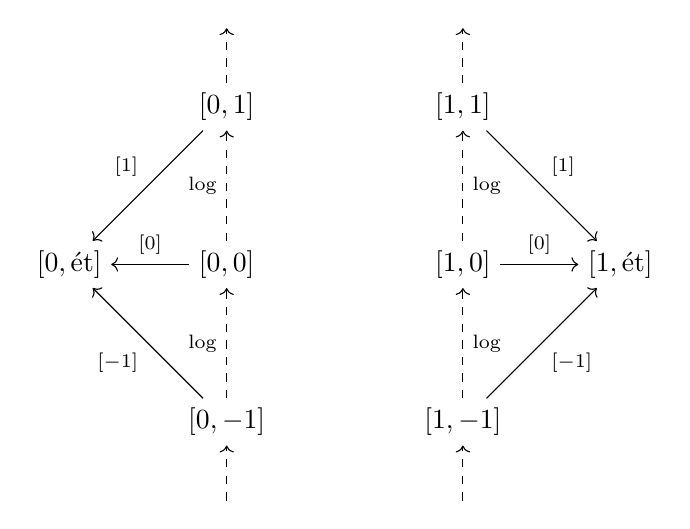
\begin{tikzpicture}[auto]
\node (L1) at (0,2) {$\LS[0,1]$}; \node (R1) at (3,2) {$\LS[1,1]$};
\node (L0) at (0,0) {$\LS[0,0]$}; \node (R0) at (3,0) {$\LS[1,0]$};
\node (L-1) at (0,-2) {$\LS[0,-1]$}; \node (R-1) at (3,-2) {$\LS[1,-1]$};
\node (Let) at (-2,0) {$\LS[0,\et]$}; \node (Ret) at (5,0) {$\LS[1,\et]$};
\draw[dashed, ->] (L1) to (0,3); %\draw[dashed] (0,3.1) to (0,3.7);
\draw[dashed, ->] (R1) to (3,3); %\draw[dashed] (3,3.1) to (3,3.7);
\draw[dashed, ->] (0,-3) to (L-1); %\draw[dashed] (0,-3.6) to (0,-3);
\draw[dashed, ->] (3,-3) to (R-1); %\draw[dashed] (3,-3.6) to (R-1);
\draw[dashed, ->] (L-1) to node {$\scriptstyle \log$} (L0);
\draw[dashed, ->] (L0) to node {$\scriptstyle \log$} (L1);
\draw[dashed, ->] (R-1) to node[swap] {$\scriptstyle \log$} (R0);
\draw[dashed, ->] (R0) to node[swap] {$\scriptstyle \log$} (R1);
\draw[->] (L-1) to node {$\scriptstyle \Kmm[-1]$} (Let);
\draw[->] (L0) to node[swap] {$\scriptstyle \Kmm[0]$} (Let);
\draw[->] (L1) to node[swap] {$\scriptstyle \Kmm[1]$} (Let);
\draw[->] (R-1) to node[swap] {$\scriptstyle \Kmm[-1]$} (Ret);
\draw[->] (R0) to node {$\scriptstyle \Kmm[0]$} (Ret);
\draw[->] (R1) to node {$\scriptstyle \Kmm[1]$} (Ret);
\end{tikzpicture}
\caption{Log and Kummer maps between log-shells}
\label{fig:logKummerMaps}
\end{figure}

Here, $\Kmm$ denotes the Kummer isomorphisms from Frobenius-like log-shells to \'etale-like log-shells.
This diagram is far from commutative, but it indicates that the contents of the log-shells of type (HF) in the log sequence on each side can be controlled by the common log-shell of type (HE) on the respective side.


\subsubsection{Upper Semi-Compatibility and \(\IndThree\)}\label{subsub:upperSemiComp}
To put it in terms of Mochizuki’s explanation, the role of the log-Kummer correspondence is to control, within the entire log sequence, the Frobenius-like unit part that shifts one step at a time through the iteration of the \(\log\)-link. The multiradial algorithm in Theorem 3.11, in broad terms, attempts to reconstruct the structure on the value-group side, such as an integral structure, from the {\'e}tale-unit part; therefore, the unit part appears in a position shifted by one step via the \(\log\)-link. To extract the invariant part with respect to this one-step shift, Mochizuki adopts the approach of treating the log sequence itself as a single vertical column and handling it as a single object; cf.\ \cite[Introduction, pp.\ 408--410]{MR4225475}.

Mochizuki emphasizes that, although the \(\log\)-link and the Kummer isomorphism are not commutative, the log-shell acts as an upper-bound that simultaneously contains their images. Mochizuki refers to this property as “upper semi-commutativity” in the log-Kummer correspondence, or “upper semi-compatibility” between the \(\log\)-link and the Kummer isomorphisms.

The third indeterminacy \(\IndThree\) arises from this log-Kummer correspondence. Specifically, it is formulated as an upper-bound constraint in such a way that, even after undergoing a shift by the \(\log\)-link, all required images remain within the log-shell. See \cite[Rem.~1.2.2(iii), pp.\ 442--443; Thm.~3.11(ii), pp.\ 575--577]{MR4225475}.



\setcounter{equation}{0}
\section{On the logic from theorem 3.11 to corollary 3.12}\label{sec:from3.11To3.12}

\subsection{Procedure on the big-H diagram}\label{sub:procedureOnBigH}
In this section, based on the discussion so far, we will outline the process for deriving Corollary 3.12 from Theorem 3.11 in the third IUT paper \cite{MR4225475}. Here, we will attempt to illustrate as concretely as possible---yet schematically---how this argument is carried out on the big-H diagram (Figure \ref{fig:BigHdiagram}).

\subsubsection{\emph{Starting point}}\label{subsub:startingPoint}

We start from the \(q\)-pilot BPS inside \(\HT[1,0]\).
The procession-normalized log-volume of the \(q\)-pilot object
\[
  -|\log(\uuqq)|\in\bR
\]
is computed in the usual way in the right-hand column. According to Mochizuki, the following procedure may be regarded as another but equivalent way of calculating this value:

\begin{quote}
The proof of Corollary 3.12 [...] is based on the
following {\it fundamental observation}: the {\bf multiradial
representation} discussed above yields  
\smallskip
\begin{center}
    {\it {\bf two tautologically equivalent} ways to compute}\\
    {\it the {\bf $\bm{q}$-pilot log-volume} $-|\log(\uuqq)|$} [.] (\cite[p.\ 421]{MR4225475})
\end{center}
\end{quote}


\subsubsection{\emph{Reading the same underlying abstract BPS from the left-hand side by the \(\Th\)-link}}\label{subsub:fromLeft}
The \(\Th\)-link glues the rigidified \(q\)-pilot BPS on the right-hand side full poly-isomorphically to the \(\Th\)-pilot BPS on the left-hand side.
They are related as two rigidifications of sufficiently weakened abstract prime-strip data.

\subsubsection{\emph{Executing Theorem 3.11 in the left-hand column}}
Apply the multiradial algorithm of Theorem 3.11 to the BPSs that appear in the \(\Th\)-link.  
By this, regions $\{\prescript{0,0}{}{U}_{\lambda}\}_{\lambda}$ of possible images of the \(\Th\)-pilot object are obtained inside $\VC(\oOOxmu[0,0]_{\uv})$, which may be identified with the large volume container associated to log-shell at $(0, 1)$.
Here, $\oOOxmu[0,0]_{\uv}$ is regarded as a log-shell, that is, as a log-shell $\LS_{\uv}(\cFvxmu)$ of type (MF) (\S\ref{subsub:MF}).


\subsubsection{\emph{Moving to the right-hand column by \'etale-picture permutation symmetries}}
The collection of regions obtained as the output of the algorithm of Theorem 3.11 lies in the large volume container associated to $\oOOxmu[0,0]_{\uv}$, which may be regarded as the log-shell at $(1, 1)$. 
Since, under the $\Th$-link, the unit group portions $\oOOxmu[0,0]_{\uv}$ and $\oOOxmu[1,0]_{\uv}$ are identified, one may regard the output of Theorem 3.11 as lying in the large volume container given by the log-shells associated to $\oOOxmu[1,0]_{\uv}$.
We write the collection of regions thus obtained as $\{\prescript{1,0}{}{U}_{\lambda}\}_{\lambda}\subset\VC(\oOOxmu[1,0]_{\uv})$.

\begin{rem}\label{rem:APT}
According to the following excerpt, the transformation from $\{\prescript{0,0}{}{U}_{\lambda}\}_{\lambda}$ to $\{\prescript{1,0}{}{U}_{\lambda}\}_{\lambda}$ can also be interpreted as the result obtained on the right-hand side by simultaneously executing the algorithm:

\medskip
\begin{quote}
[The] construction algorithm may be expressed in terms that are
{\bf simultaneously} valid/executable/well-defined relative to {\bf both}
the {\it arithmetic holomorphic structure} that gives rise to the {\it
$\Th$-pilot object} in the {\it domain} of the $\Th$-link {\bf and} the
{\it arithmetic holomorphic structure} that gives rise to the {\bf input
data prime-strip} [.] (\cite[Rem.\ 3.11.1(v), p.\ 585]{MR4225475})
\end{quote}
\end{rem}


\subsubsection{\emph{Reading through the log-Kummer correspondence in the right-hand holomorphic structure}}
The collection of regions $\{\prescript{1,0}{}{U}_{\lambda}\}_{\lambda}$ lies in the large volume container associated to the log-shells $\oOOxmu[1,0]_{\uv}$.
We identify $\oOOxmu[1,0]_{\uv}$ (up to $\Ind_2$) with the one obtained as the subquotient of $\oK[1,0]_{\uv}$, apply the log function once to form the log-shell $\LS[1,1]=\LS[1,1](\cF)$ of type (HF), and regard $\{\prescript{1,0}{}{U}_{\lambda}\}_{\lambda}$t as lying in the large volume container associated to $\LS[1,1]$.
We write the collection of regions thus regarded as $\{\prescript{1,1}{}{U}_{\lambda}\}_{\lambda}\subset\VC(\LS[1,1])\otimes\bQ$.


\subsubsection{\emph{Taking the holomorphic hull}}
Taking the union of the possible image regions $\{\prescript{1,1}{}{U}_{\lambda}\}_{\lambda}$, one takes the holomorphic hull (with respect to the ring structure at $(1, 1)$) 
\[
  \prescript{1,1}{}{U}^{\hol}\subseteq\VC(\LS[1,1])
\]
and then takes the normalized determinant to obtain an arithmetic line bundle $(\prescript{1,1}{}{U}^{\hol})^{\det}$ (with respect to the ring structure at $(1, 1)$).


\subsubsection{\emph{Ladder argument}}
Up to this point, we have argued by placing a $\Th$-link $\HT[0,0]\stackrel{\text{$\Th$-link}}{\to}\HT[1,0]$ between $\HT[0,0]$ and $\HT[1,0]$.
In general, for every integer $m$, one places a $\Th$-link $\HT[0,m]\stackrel{\text{$\Th$-link}}{\to}\HT[1,m]$ between $\HT[0,m]$ and $\HT[1,m]$ and carries out the same argument.
This yields, with the $q$-pilot BPS of $\HT[1,m]$ as input, the $\Th$-pilot arithmetic line bundle $(\prescript{1,m+1}{}{U}^{\hol})^{\det}$ in $\HT[1,m+1]$.

If one regards the right-hand log sequence $\HT[1,\ast]$ as a single object, then one has obtained an algorithm that obtains a diagonal line bundle $(\prescript{1,\Delta}{}{U}^{\hol})^{\det}$ from the diagonal $q$-pilot BPS $\BPS[1,\Delta]_q$.


\subsubsection{\emph{Taking the log-volume}}\label{subsub:fromLeftVol}
Take the procession-normalized log-volume of $(\prescript{1,\Delta}{}{U}^{\hol})^{\det}$.
The value $\logvol((U^{\hol})^{\det})$ is \(-|\log(\Th)|\).


\subsubsection{\emph{Attempt to reach a conclusion}}\label{subsub:finalArgument}
Mochizuki asserts that, by properties of the algorithm itself such as (IPL), (SHE), and (APT), discussed below, the procedure from \S\ref{subsub:fromLeft} to \S\ref{subsub:fromLeftVol} becomes a way of calculating, with indeterminacies, the real number $-|\log(q)|$, which is independent of the way of calculating the real number $-|\log(q)|$ in \S\ref{subsub:startingPoint}.  
He further asserts that, on the basis of this, one can construct a proof that obtains the inequality of Corollary 3.12
\begin{equation}\label{eqn:Cor312FinalInequality}
  -|\log(\uuqq)|\leq -|\log(\uuTh)|.
\end{equation}


\subsection{(IPL), (SHE), (APT)}\label{sub:IPLSHEAPTPrecise}
Here let us organize, in the terminology of the present paper, the three properties (IPL), (SHE), and (APT) used in the preceding subsection.

\medskip\noindent
According to Mochizuki, {\bf (IPL)}\ \emph{input prime-strip link} is the property that 

\medskip\begin{quote}
[the] output data is constructed in such a way that it is {\bf
linked/related}, via full poly-isomorphisms of {\bf
$\bFmrts$-prime-strips} induced by operations in the algorithm, to the
{\bf input data prime-strip}, i.e., the {\bf ``coric''/``fixed''
$\bm{q}$-pilot $\bFmrts$-prime-strip}, equipped with its {\it rigidifying}
{\bf arithmetic holomorphic structure} [...]. (\cite[Rem.\ 3.11.1(iii), p.\ 582]{MR4225475})
\end{quote}

\medskip
This can be almost word-for-word translated as: the intermediate BPS of type $I$ that appears in the process of constructing the output region \(U_{\lambda}\) of Theorem 3.11 is linked, by the full poly-isomorphism, to the input-data prime-strip, that is, to the \(q\)-pilot BPS in the right-hand column.


\begin{rem}
However, we remark that the assertion that two BPSs are ``linked,'' in the sense that there exists an isomorphism between them, is a vacuous assertion since the category of BPSs is a connected groupoid. 
Therefore, the concept of a ``link'' needs a more precise definition that can be formalized in Lean.
\end{rem}


\medskip\noindent
According to Mochizuki, {\bf (SHE)}\ \emph{simultaneous holomorphic expressibility} is the property that 

\medskip
\begin{quote}
[the] construction of this output data, as well as the output data itself,
is expressed in terms that are {\bf simultaneously}
valid/executable/well-defined relative to {\bf both}

\smallskip
\begin{quote}
the {\bf arithmetic holomorphic structure} that gives rise to the {\bf
$\Th$-pilot object} in the {\it domain} of the $\Th$-link---i.e., in
more technical language, in terms of/as a {\bf function} of structures in
the $\Th^{\pm\text{ell}}$NF-Hodge theater in the domain of the $\Th$-link---
\end{quote}

\smallskip
{\bf and}

\smallskip
\begin{quote}
the {\bf arithmetic holomorphic structure} that gives rise to the {\bf
input data prime-strip} [...] in the {\it codomain} of the 
$\Th$-link---i.e., in more technical language, in terms of/as a {\bf
function} of structures in the $\Th^{\pm\text{ell}}$NF-Hodge theater in the codomain of
the $\Th$-link. (\cite[Rem.\ 3.11.1(iii), p.\ 583]{MR4225475})
\end{quote}
\end{quote}

\medskip
That is, in our wording, the output construction and output regions of Theorem 3.11 are expressed by words that are simultaneously valid/executable/well-defined not only with respect to the ring-theoretic background on the domain side, which produces the \(\Th\)-pilot object, but also with respect to the ring-theoretic background on the codomain side, which produces the input-data prime-strip, that is, the \(q\)-pilot object. 


\medskip\noindent
{\bf (APT)}\ \emph{algorithmic parallel transport} is the property that\footnote{Here, we can think of a ``tensor packet'' as what we call a ``large volume container.''} 

\medskip
\begin{quote}
[the] parallel transport mechanism does {\bf not} consist of a simple
instance of transport of {\it some set-theoretic region} [such as the
region in the tensor packet of log-shells determined by the {\it
$\Th$-pilot object} in the {\it domain} of the $\Th$-link] {\it via some
set-theoretic function}.  Rather, it consists of a {\bf construction
algorithm} that is {\bf simultaneously valid/executable/well-defined} with
respect to the arithmetic holomorphic structures in the domain and
codomain of the $\Th$-link [...]. (\cite[Rem.\ 3.11.1(iv), p.\ 584]{MR4225475})
\end{quote}

\medskip
Although this is not explicitly stated in the original IUT paper, this property appears to be the main basis for the excerpt from Remark \ref{rem:APT}.



\subsection{From theorem 3.11 to corollary 3.12}\label{sub:fromThm311toCor312Precise}
Based on the properties described above, from Theorem 3.11 to Corollary 3.12, especially the final part of the argument, can be interpreted, broadly speaking, as follows (cf.\ \cite[Proof of Cor.\ 3.12, Step (xi), pp.\ 606ff]{MR4225475}).

\medskip
Fix the \(q\)-pilot object in the right-hand column \(\HT[1,0]\).
Its log-volume is computed by the native holomorphic structure as \(-|\log(q)|\).
On the other hand, by the \(\Th\)-link, this \(q\)-pilot prime-strip is linked full poly-isomorphically to the \(\Th\)-pilot prime-strip in the left-hand column.

When Theorem 3.11 is applied to the \(\Th\)-pilot object in the left-hand column, one obtains regions \(\{\prescript{0,0}{}U_{\lambda}\}\) of possible images of the \(\Th\)-pilot object.
These regions are indexed by \(\IndOne\), \(\IndTwo\), and \(\IndThree\).
By \'etale-picture permutation symmetries and the log-Kummer correspondence, this output region is expressed as a region \(\{\prescript{1,1}{}U_{\lambda}\}\) in the right-hand column.

\begin{itemize}
\item Here, by (IPL), the construction of \(\{\prescript{1,1}{}U_{\lambda}\}\) is linked to the right-hand \(q\)-pilot input prime-strip.
\item Also, by (SHE), \(\{\prescript{1,1}{}U_{\lambda}\}\) is expressible in the language of the holomorphic structure of \(\HT[1,0]\), and is moreover compatible with the condition that the \(q\)-pilot log-volume is fixed as \(-|\log(\uuqq)|\).
\item Furthermore, by (APT), the passage above is justified not as a set-theoretic transport that identifies the ring structures on the two sides, but as an algorithmic parallel transport executed simultaneously with respect to coric data.
\end{itemize}

Then, accordiong to Mochizuki's interpretation (\cite[Step (xi) of the proof of Cor.\ 3.12]{MR4225475}), the IPL, SHE, and APT properties implies that the set of procession-normalized log-volumes of the admissible output regions contains the $q$-pilot log-volume as one of its possible values.
That is,
\[
  -|\log(\uuqq)|\in \bR_{\leq -|\log(\uuTh)|}.
\]
By the definition of \(\bR_{\leq -|\log(\uuTh)|}\), this means
\[
  -|\log(\uuqq)|\leq -|\log(\uuTh)|.
\]

\begin{rem}\label{rem:twoTautologicalWays}
In Mochizuki's explanation, the core of the proof of Corollary 3.12 is expressed by saying that ``two tautologically equivalent ways'' of calculating the \(q\)-pilot log-volume \(-|\log(\uuqq)|\) are obtained.
In the terminology of the present paper, the first calculation is the direct calculation of the \(q\)-pilot log-volume by the ring structure that arises from the right-hand column.  
The second calculation is the calculation that reads the \(q\)-pilot log-volume as a possible log-volume of the \(\Th\)-pilot output region by passing through the \(\Th\)-link, the multiradial algorithm of Theorem 3.11, the log-Kummer correspondence, and the holomorphic hull.
It is asserted that, as a result of the ladder argument, these two calculations meet inside the same right-hand volume container, and \eqref{eqn:Cor312FinalInequality} follows.
\end{rem}


\setcounter{equation}{0}
\section{Points to be clarified}\label{sec:pointsToClarify}
As is clear from the discussion so far in this article, we are reserving our final judgment on whether a proof exists for Corollary 3.12 in Mochizuki's third paper on IUT theory \cite{MR4225475}.
The reason for this is that there are parts of the proof's argument—namely, the reasoning leading from Theorem 3.11 to Corollary 3.12—that we have not been able to fully follow.

In this section, we will briefly describe these ``parts we have not been able to follow'' in as simple terms as possible.
Although this is stated in simple terms, it has not been essentially simplified.
We believe that if the problem described in the ``main goal'' below is solved, then Corollary 3.12 (and thus, in particular, the abc conjecture) will follow.

``The $\eta$ algorithm'' described below is essentially the same as the ``Theorem 3.11 algorithm'' described in \S\ref{sub:procedureOnBigH}, but it is a rephrasing of the algorithm in a context that does not explicitly deal with the big-H diagram.


\subsection{The $\eta$ algorithm}\label{sub:etaAlgorithm}

\begin{figure}
\begin{tikzpicture}[font=\footnotesize, node distance=12mm and 14mm]
  % Top chain
  \node (Pi) {$\PPi_{\uv}$};
  \node (PimY) [right=of Pi] {$\PPi_{{\uv},\dduuY}$};
  \node (M) [below=36pt of Pi] {$M$};
  \node (Minfty) [below=32ptof PimY] {$M_\infty$};
  \node (H1) [right=of Minfty] {${}_\infty H^1(\PPi_{{\uv},\dduuY},\Lambda(M_\infty))$};
  \node (H1rig) [right=of H1] {${}_\infty H^1(\PPi_{{\uv},\dduuY},\ell \cdot \Delta^c)$};

  \draw[->] (PimY) -- node[above]{\scriptsize $\supset$} (Pi);
  \draw[->] (Pi) -- node[left]{\scriptsize $\acton$} (M);
  \draw[->] (PimY) -- node[left]{\scriptsize $\acton$} (Minfty);
  \draw[->] (M) -- (Minfty);
  \draw[->] (Minfty) -- node[above]{Kummer} (H1);
  \draw[->] (H1) -- node[below]{\scriptsize $\sim$} node[above]{\scriptsize $\Lambda$-rigidity} (H1rig);
  \node (ProdH1Dt) [below left=22mm and 10mm of H1rig] {$\prod_t {}_\infty H^1(D_{t,\uv},\ell \cdot \Delta^c)$};
  \node (ProdOt) [below=18mm of ProdH1Dt] {$\prod_t \oOOt_{t,\uv}$};
  \node (ProdLog) [right=18mm of ProdOt] {$\prod_t \log(\oOOxmu_{t,\uv})$};
  \draw[->] (H1rig) -- node[midway, sloped, below]{\scriptsize Galois evaluation} (ProdH1Dt);
  \draw[->] (ProdOt) -- (ProdH1Dt);
  \draw[{Hooks[right]}->] (ProdOt) -- (ProdLog);
  \draw[dashed,->] (Minfty) .. controls +(0mm,-12mm) and +(-18mm,10mm) .. (ProdOt);
\end{tikzpicture}
\caption{The $\eta$ algorithm}
\end{figure}

We start with a BPS, say $\cB = (\{\GG_{\uv}\acton M_{\uv}\},\cC)$.
We proceed as follows:
\subsubsection{Step 1}
Choose an isomorphism between the given BPS and the $\Th$-pilot BPS (\S\ref{subsub:ThPilotBPS}) associated to a Hodge theater $\HT$.
This gives us, at each place $\uv$, the action on a monoid
\[ \Pi_{\uv} \acton \Th^{\bN}\times\oOOx_{\uv}, \]
where $\Th$ is a formal symbol (as that in the $\Th$-pilot BPS (\S\ref{subsub:ThPilotBPS})) that represents the generator of $\bN$ acting on the right-hand monoid by ``powers.''

\subsubsection{Step 2}
Use an anabelian algorithm to determine the subgroup $\Pi_{v,\dduuY}$ and a natural action on 
\[ M_\infty \eqdef \Th^{\bQ_{\geq 0}}\times \oOOx_{\uv} \]
which is compatible with the previous action.

\subsubsection{Step 3}
The torsion in $M_\infty$ is isomorphic to $\bQ/\bZ$ and thus the adic Tate module (with the action of $\Pi_{v,\dduuY}$) provides a ``cyclotome'' $\La(M_\infty)$ as well as a canonical ``Kummer'' map
\[ M_\infty \longto H^1(\Pi_{\uv,\dduuY},\La(M_\infty)). \]

\subsubsection{Step 4}
There is an anabelian algorithm that constructs the geometric part of $\Pi_{v,\dduuY}$, say $\Delta$. 
Put 
\[ \Delta^c \eqdef \frac{[\Delta,\Delta]}{[\Delta,[\Delta,\Delta]]}. \]
This is isomorphic to $\hbZ$, and there is a canonical isomorphism (the ``cyclotomic rigidity isomorphism''; cf.\ \S\ref{sub:cyclotomicRigidity}) of type
\[ \La(M_\infty) \cong \ell \cdot \Delta^c, \]
compatible with the action of the fundamental group.
We consider the composition of the above Kummer map with this map to obtain 
\[ M_\infty \longto \infH^1(\Pi_{\uv,\dduuY}, \ell \cdot \Delta^c). \]

\subsubsection{Step 5}
We recover decomposition groups $(D_{t,\uv})_t$ in some anabelian way (cf.\ \S\ref{subsub:GaloisEvaluation}) inside of $\Pi_{\dduuY}$, and restrict to obtain 
\[ \infH^1(\Pi_{\uv,\dduuY},\ell \cdot \Delta^c) \longto \prod_t \infH^1(D_{t,\uv},\ell \cdot \Delta^c). \]

\subsubsection{Step 6}
Using another cyclotomic rigidity isomorphism, and some synchronization (cf.\ \S\ref{subsub:thetaValActStep6}), we obtain \[ \prod_t \oOOt_{\uv,t} \longto \prod_t \infH^1(D_{t,\uv},\ell \cdot \Delta^c), \] and one proves that the map from $M_\infty$ described above actually factors through this $\prod_t \oOOt_{\uv,t}$. 
Here, note that, as in \S\ref{subsub:thetaValActStep6}, $\oOOt_{\uv,t}$'s should be read as a component of a certain container of the splitting monoid (Gaussian monoid) \cite[Cor.\ 4.10(i), pp.\ 384--385]{MR4225474}.

\subsubsection{Step 7}
$\prod_t \OOt_{\uv,t}$ embeds in $\prod_t \oK_{\uv,t}$, which we identify with $\prod_t \oOOxmu_{\uv,t}$ via log.
This contains the log-shells $\prod_t \cI_{\uv,t}$ of type (MF).

\subsubsection{Step 8}
Putting everything together, we obtain an action of $\Th$ (via $\LGP$) on $\prod_t \cI_{\uv,t}$, and thus an action of the ``$\bN$'' part from the very beginning of the algorithm (which is contained in $M_\infty$).

\subsubsection{Step 9}
Relate the log-shells $\cI_{\uv,t}$ to those constructed from the original BPS, and consider them as if they were constructed from the original BPS in the standard way.
That is, the log-shells of type (MF) obtained from the chosen Hodge-theater realization are compared, via the Kummer isomorphisms, with the log-shells $\LS[\et]_{\uv,t}$ of type (ME) reconstructed functorially from the original \'etale-unit BPS and its compact structure. Along the log sequence this comparison is only upper semi-compatible. Hence, in this way, one can read the output in terms of the original input data in the log-shells $\LS[\et]_{\uv,t}$ with $\IndThree$-ambiguity. 


\subsection{The main goal}\label{sub:theMainGoal}
In the discussion above, we have explained how to construct an action of $\bN$ on $\VC(\cI_{\uv})$, in an anabelian way, after fixing an isomorphism between a given BPS and the $\Th$-BPS associated to a Hodge theater (and this action is thus subject to indeterminacies Ind1 and Ind2).


Once we fix $S \subset \VC(\LS_{\uv})$, this provides an isomorphism between the $\cC$ part of the original BPS (which we denote by $\bR^{val}$ \footnote{The super-script ``val'' indicates that it is a copy of $\bR$ coming from the value-group part of the BPS.}) and the $\cC$ constructed using the action and $S$ as the integral structure, which we denote by $\bR^{ss}$ \footnote{The super-script ``{\it ss}'' means, according to Mochizuki, {\it semi-simplification}.}; more precisely, 
$$
\bR^{ss}=\{T\subset\VC(\cI_{\uv})\mid \text{adelic and measurable}\}/\mathord{\sim},
$$
where $T\sim T'$ if and only if the volume of $T$ coincides with that of $T'$; we define $M=1\cdot S$ (the action of $1\in \bN$), which represents ``$\LGP\cdot S$'' (cf.\ \S\ref{subsub:actionOfTheta}), and put the class of $M$ in $\bR^{ss}$ to be the pilot.
Thus the isomorphism 
\[ \eta^{\mathrm{anab}}_S : \bR^{val} \simlongto \bR^{ss} \]
of the pointed real vector spaces depends on $S$, and is constructed via anabelian methods as discussed above.

On the other hand, when we work with a BPS that was constructed as the $q$-BPS of a Hodge theater, this perspective provides us with an isomorphism 
\[ \eta^q : \bR^{val} \simlongto \bR^{ss}, \]
where the pilot of the target $\bR^{ss}$ is given by the class of $\{q_{\uv}\OO_{\uv}\}$ embedded ``diagonally'' into the large volume container $\VC(\cI_{\uv})$.

The main goal now is to relate these two kinds of isomorphisms: the one arising from $q$ and the one arising from anabelian methods. 
Concretely, we wish to show that there exists some suitable $S$ such that 
\begin{equation}\label{eqn:SSEtaGoal}
\eta^q = \eta^{\mathrm{anab}}_S. 
\end{equation}

\subsection{Minimal structure of the $\eta$-algorithm}\label{sub:SSEtaStructure}
The input of the $\eta$-algorithm is a BPS, whose {\'e}tale-unit portion consists of actions of local Galois groups on unit monoids together with compact structures, and whose value-group portion is an oriented real line with local pilots; see \S\ref{sub:BPS}.
From the value-group portion, a real line $\bR^{val}$ with a canonical pilot was constructed. On the other hand, from the operation (multiplication) of the unit monoid, an additive object was constructed via $\log$, and from that, another real line $\bR^{ss}$ was constructed. The construction of the latter is
\[
  \text{{\'e}tale-unit portion}
  \rightsquigarrow
  \text{log-shells}
  \rightsquigarrow
  \text{volume containers}
  \rightsquigarrow
  \bR^{ss},
\]
where the arrows stand for the constructions described in \S\ref{sub:logShell}, the immediately following subsection on volume containers, \S\ref{sub:logLink}, and the present \S\ref{sec:pointsToClarify}.  

The $\eta$'s, which are isomorphisms between these two real lines, describe the relationship between the value-group portion and the \'etale-unit portion, and \eqref{eqn:SSEtaGoal} indicates that the starting point $\eta^q$ belongs to an orbit (an analogue of a Teichm\"uller deformation) generated by the indeterminacies of the formation of $\eta^{\mathrm{anab}}_S$. In other words, at the level of degree (log-volume), the rigidified $q$-pilot is represented in the output regions, and this outlines Mochizuki's strategy to obtain the desired inequality between the log-volumes.


\setcounter{equation}{0}
\section{An examination of Scholze-Stix document}\label{sec:ScholzeStixExamination}

\subsection{Scope of the examination}\label{sub:SSScope} % ``the report'' vs ``this report''

We now compare our analysis with that made by Scholze and Stix in \cite{Scholze2018WhyA}, in which the conclusion is reached that ``the suggested proof has [a problem] so severe that in
our opinion small modifications will not rescue the proof strategy.'' 
In the final part of \cite{Scholze2018WhyA}, the occurrence of monodromy in the identifications among the various ordered one-dimensional real vector spaces appearing in the theory is pointed out as a flaw in the proof \cite[pp.\ 9--10]{Scholze2018WhyA} (see Figure \ref{fig:TheScholzeStixhexagon} below).
The purpose of the present section is to put this observation in context, based on our exposition 
in \S\ref{sec:multiradialThetaCor312}--\S\ref{sec:pointsToClarify},
and to indicate why this occurrence of monodromy does not represent an obstruction to the intended proof strategy of Mochizuki.


\subsection{The Scholze-Stix hexagon}\label{sub:SSHexagon}

We reproduce the diagram from \cite[p.\ 10]{Scholze2018WhyA} in Figure~\ref{fig:TheScholzeStixhexagon}; interpret the terms of the diagram in our language; and confirm the observation made in \cite{Scholze2018WhyA} that the diagram does not commute.

\begin{figure}[ht]
\begin{center}
$$
\xymatrix{
&\bR_{\odot,\Th}\ar[dl]\ar[r]^{\text{$\Th$-link}}_{\cong}&\bR_{\odot,q}\ar[dr]\\
(\bR_{\odot_c,\Th_j})_{j=1,\ldots,\ell^{\divideontimes}}\ar[dr]&&&\bR_{\odot_c,q}\ar[dl]\\
&\bR_{\Th}\ar[r]_{=}&\bR_{q}
}
$$
\caption{The Scholze-Stix hexagon}
\label{fig:TheScholzeStixhexagon}
\end{center}
\end{figure}

In the language of \cite{Scholze2018WhyA}, the entries at the top level of the diagram are ``abstract pilots''; the entries at the middle level of the diagram are ``concrete pilots''; and the entries at the bottom level of the diagram are identical copies of $\mathbb{R}$.
We have translated the precise definitions of these entries into our language;
the result can be found in the following table. 

\begin{table}[ht]
    \centering
    \begin{tabular}{|c|c|}
        \hline
         Scholze-Stix & LANA \\ \hline\hline
        $\bR_{\odot,\Th}$ &
        \begin{minipage}{20em}

        \medskip
        the $\Th$-pilot value-group BPS viewed as
        an object abstractly isomorphic to
        the $q$-pilot value-group BPS

        \medskip
        \end{minipage}\\ \hline
        $\bR_{\odot,q}$ &
        \begin{minipage}{20em}

        \medskip
        the $q$-pilot value-group BPS viewed as
        an object abstractly isomorphic to
        the $q$-pilot value-group BPS

        \medskip
        \end{minipage}\\ \hline
        $\bR_{\odot_c,\Th_j}$ &\begin{minipage}{20em}

        \medskip
        the ``$j$th-component'' of the $\Th$-pilot value-group BPS

        \medskip
        \end{minipage}\\ \hline
        $\bR_{\odot_c,q}$ &
        \begin{minipage}{20em}

        \medskip
        the $q$-pilot value-group BPS

        \medskip
        \end{minipage}\\ \hline
        $\bR_{\Th}$ and $\bR_{q}$ &
        \begin{minipage}{20em}

        \medskip
        identical copies of the real line $\bR$

        \medskip
        \end{minipage}\\ \hline
    \end{tabular}

    \bigskip
    \caption{Definitions of the entries in Figure \ref{fig:TheScholzeStixhexagon}}\label{tab:dictionary}
\end{table}

In \cite{Scholze2018WhyA}, each of these one-dimensional real vector spaces is regarded as a \textit{pointed} space; all of the arrows in the diagram are morphisms of pointed vector spaces except for the diagonal arrows from the middle row to the bottom row, which are degree maps.
The composition $\bR_{\odot,\Th} \to \bR_{\Th}$ scales by a factor of
\[
\frac{1}{\ell^{\divideontimes}} (1^2 + 2^2 + \cdots + (\ell^{\divideontimes})^2)
\]
while the composition $\bR_{\odot,q} \to \bR_q$ scales by a factor of 1.

From this we may conclude that \textit{if} the deduction of \cite[Cor.\ 3.12, pp.\ 597--598]{MR4225475} 
from \cite[Thm.\ 3.11, pp.\ 573--580]{MR4225475} could be phrased in a manner that factors through a diagram as in
Figure \ref{fig:TheScholzeStixhexagon}, then one would have to repair commutativity by introducing a factor of $O(\ell^2)$. This would render the final inequality powerless to prove a conclusion as strong as the $abc$ conjecture. 

In our understanding, however, the inequality in \cite[Cor.\ 3.12, pp.\ 597--598]{MR4225475} is not obtained by comparing the volumes of two pilots situated on the two sides of the $\Th$-link. Rather, it is obtained by comparing the degree of arithmetic line bundles within the arithmetic holomorphic structure on one side of the $\Th$-link. Thus, the non-commutativity of the diagram in Figure \ref{fig:TheScholzeStixhexagon} does not, by itself, establish a defect in the intended proof strategy.

\subsection{Comparison of approaches}\label{sub:SSActualComparison}

We now explain the required comparison in terms of our presentation in \S\ref{sec:pointsToClarify}.
As indicated there, the proof of Corollary 3.12 rests on the comparison \eqref{eqn:SSEtaGoal}
in which the two maps have different construction processes.  The map $\eta^q$ is obtained from the $q$-pilot together with the native arithmetic holomorphic structure of the $q$-side.  The map $\eta^{\mathrm{anab}}_S$ is obtained by starting from a weakened BPS, reconstructing the relevant action by anabelian and Kummer-theoretic procedures, and selecting suitable integral-structure data $S$ inside the product of log-shells.  Both are then intended to be read in the same semiring/log-shell target $\bR^{\mathrm{ss}}$, with the source identifications stipulated in \S\ref{sub:theMainGoal}. 

The analysis of Scholze-Stix compresses these construction processes down to
abstract generators, concrete divisors, and trivialized real lines.
By contrast, \eqref{eqn:SSEtaGoal} asserts a comparison of two constructions \textit{before} computing degrees; only after such a comparison has been established can one pass to a common volume container where one can compare normalized log-volumes. 
In Mochizuki's original argument, the final inequality is obtained by comparing the log-volume of the $q$-pilot object at $\HT[1,0]$ with the log-volume of the region $(\prescript{1,\Delta}{}{U}^{\hol})^{\det}$; these two objects lie on the \textit{same} side of the $\Th$-link, i.e., the right-hand side of the $\Th$-link.  

Viewing from a different perspective, Scholze-Stix seems to try to identify, in a coherent manner, the copies of $\mathbb{R}$ arising from the two sides of the $\Th$-link in order to obtain a ``common ground'' (i.e., common $\bR$) for comparing the log-volumes of objects lying on opposite sides of the $\Th$-link.
According to Mochizuki, however, IUT provides two distinct ways of computing the log-volume of the $q$-pilot object:\ the usual computation and the computation via the multiradial algorithm. It is important to note that the role of the $\Th$-link is not to enable a direct comparison of numerical invariants lying on its two sides. Note also that Mochizuki asserts that the multiradial algorithm may be established by considering, e.g., the indeterminacy $\IndThree$ and the \'etale-unit portions ``$\GG_{\uv} \acton \oOOxmu_{\uv}$,'' which were not discussed by Scholze-Stix.  


\subsection{The effect of ``blurring''}\label{sub:SSBlurringNew}

At the end of their report \cite[p.~10]{Scholze2018WhyA}, Scholze-Stix say that Mochizuki claimed commutativity ``up to the `blurring' given by certain indeterminacies,'' and they infer a ``factor of at least $O(\ell^2)$'' that would make the inequality useless. 
The report gives no separate mathematical definition of ``blurring'';
from context one may infer that this is meant to refer to the effects of $\IndOne$, $\IndTwo$, and $\IndThree$, but \cite{Scholze2018WhyA} works with a compression in which the \'etale-unit data, the log-Kummer correspondence, and the three indeterminacies are not represented separately to describe these effects precisely. In any case, the conclusion about a ``factor of at least $O(\ell^2)$'' seems to depend on the predicate that the derivation of the final equality depends on reconciling the diagram in Figure~\ref{fig:TheScholzeStixhexagon}.

The wording in \cite{Scholze2018WhyA} further suggests that $\IndOne$, $\IndTwo$, and $\IndThree$ act directly on the real numbers appearing in Corollary~3.12. In our interpretation, these effects occur elsewhere: the indeterminacies create ambiguities in the choice of the set $S$ in \eqref{eqn:SSEtaGoal}. These ambiguities are reflected in the log-volume calculation for the hull in IUT IV \cite{MR4225476}; this calculation is made at each place individually, but the effects of $\IndOne$, $\IndTwo$, and $\IndThree$ cannot be detected locally (as one would reasonably expect from the  fact that the desired diophantine inequality is not a purely local phenomenon). This description also suggests that the indeterminacies must be carefully managed so as to keep the log-volume of the hull small enough to yield a meaningful inequality.


\subsection{Provisional assessment}\label{sub:SSAssessmentNew}

To reiterate, we concur that the diagram in Figure~\ref{fig:TheScholzeStixhexagon} does not commute,
and that repairing it would require a rescaling factor that is too large to yield a proof of the $abc$ conjecture. Indeed, this point was also made by Mochizuki in his response to \cite{Scholze2018WhyA} 
(see \cite[\S 12, (IUAD)]{Mochizuki2018}): ``[this situation] occurs whenever one works within a single
holomorphic structure/ring theory.''

On the other hand, our analysis does not give rise to this particular diagram;
rather, the elaboration of the $\eta$-algorithm shows that the proof of the final numerical inequality hinges on the compatibility \eqref{eqn:SSEtaGoal} which is not manifestly false.
However, we, the LANA project, do not have a proof of \eqref{eqn:SSEtaGoal} at this time.


Of course, it should be noted here that there are also several points in common between our analysis and that of Scholze-Stix. Perhaps the most important common point is that both reports point out a problem in the ``process of deriving Corollary 3.12 from Theorem 3.11,'' and that this issue relates to the ``identification of copies of the real number line $\bR$.'' However, to elaborate further on the former point, although Scholze-Stix went on to argue that ``the suggested proof has [a problem] so severe that, in [their] opinion, minor modifications will not rescue the proof strategy,'' we are not making any claims regarding the possibility or difficulty of remedying. Furthermore, regarding the question of whether a proof of the ``$abc$ Conjecture'' exists, while many LANA members hold the view that ``the original paper does not contain at least a {\it formalizable} proof,'' the members were unable to reach complete consensus on this point.


\frenchspacing
\bibliographystyle{plain}
\bibliography{LANA}


\bigskip\bigskip\noindent
{\small
Core members of LANA Project:

\medskip\noindent
Fumiharu Kato (Leader; ZEN university)

\smallskip\noindent
Johan Commelin (Utrecht University)

\smallskip\noindent
Yuichiro Hoshi (Research Institute for Mathematical Sciences, Kyoto University)


\smallskip\noindent
Kiran Kedlaya (University of California, San Diego)

\smallskip\noindent
Adam Topaz (University of Alberta;)

\bigskip\bigskip\noindent
Corresponding author 

\medskip\noindent
Fumiharu Kato

\noindent
Faculty of Social Informatics, ZEN university

\noindent
3-12-11 Shinjuku, Zushi City, Kanagawa 249-0007, Japan

\noindent
Email: \email{\tt fumiharu\_kato@zen.ac.jp}
}


\end{document}
